
The previous chapter discussed automated methods to obtain the data to train content based classifiers. For annotated online content (such as Flickr images) however, it may be more important to assign good quality tags with the content. This chapter discusses methods to do that, through addressing sparsity of tags associated with online content. 


Several expert systems have been proposed to address the sparsity of tags associated with online content such as images and videos. However most of such systems either necessitate extracting domain-specific features, or are solely based on tag semantics, or have significant space requirements to store corpus based tag statistics. To address these shortcomings, in this work we show how ontological tag trees can be used to encode information present in a given corpus pertaining to interaction between the tags, in a space efficient manner. An ontological tag tree is defined as an undirected, weighted tree on the set of tags where each possible tag is treated as a node in the tree. We formulate the tag tree construction as an optimization problem over the space of trees on the set of tags and propose a novel local search based approach utilizing the co-occurrence statistics of the tags in the corpus. To make the proposed optimization more efficient, we initialize using the semantic relationships between the tags. The proposed approach is used to construct tag trees over tags for two large corpora of images, one from Flickr and one from a set of stock images. Extensive data-driven evaluations demonstrate that the constructed tag trees can outperform previous approaches in terms of accuracy in predicting unseen tags using a partially observed set of tags, as well as in efficiency of predicting all applicable tags for a resource. 



\section{Introduction} \label{sec:Introduction}
The consumer electronic revolution and the Internet have led to the availability of vast amounts of data including multimedia data such as images and videos. A significant fraction of such data is user generated content, in the form of pictures and videos uploaded onto sites such as Facebook~\cite{Facebook}, Flickr~\cite{Flickr} and YouTube~\cite{Youtube}. Owing to the fact that there are minimal requirements when uploading the content and that mobile uploads are on the rise, users rarely add any extra information such as a textual description to the content. At best, most images and videos are {\em tagged} with certain keywords. As these keywords or tags are sometimes applied to entire albums of images or videos at once, or applied in error, the information provided by such tags is quite noisy. %We define noisy tags as ones that would not be associated with a given image, as per a trained human annotator, without any contextual information in addition to the visual information provided in the image. 
\begin{figure}[htp]
\centering
\begin{tabular}{p{3cm} p{3cm} p{3cm}}
\centering
\epsfig{width=1.5cm,height=2.1cm,figure=TagTree/figures/4670326818_bf12bf1525.eps} &
\epsfig{width=1.5cm,height=2.1cm,figure=TagTree/figures/252474171_7f272001c5.eps} &
\epsfig{width=2.1cm,height=1.5cm,figure=TagTree/figures/5835556089_812a272a59.eps}\\
(a) `animal', {\bf `car'}  & 
(b){\bf `wedding'}, `mushroom' & 
(c) `farms', {\bf `snow'} 
\end{tabular}
\caption{Examples of incorrect tags given by users on {\tt www.flickr.com}. (a) An image of a `cat' tagged as `car', which most likely is a spelling mistake, (b) an image of a `mushroom' also tagged as `wedding' and (c) an image of a `goat' tagged with `snow'. The Flickr owner and photo ids of these images are (8656572@N04,4670326818), (35468147887@N01,252474171), (39405339@N00,5835556089) respectively.}
\label{fig:flickrnoise}
\end{figure}
%\hspace{-2cm}
Some examples of images having incorrect tags (as per human experts) are shown in Fig.~\ref{fig:flickrnoise}. The massive scale of data and the lack of useful metadata makes it difficult for users to access data that may be of interest to them~\cite{DeepaFolkso14},\cite{ShuhuiAuthor15},\cite{ZhengRecom10}. 
%. This is commonly refered to as information overload in literature.


The social tagging at the above mentioned data sharing websites creates a {\em Folksonomy}~{\cite{HsiehCollab09},\cite{SunLang11},\cite{HyunwooFrame14}} which mitigates the information overload to some extent by creating non-hierarchical categories or indexes for the retrieval of data. Folksonomies make it scalable to assign labels to large volumes of data in a collaborative manner and are hence more appropriate for such data than traditional taxonomies established by expert cataloguers~{\cite{HyunwooFrame14}}. At the same time, collaboratively produced folksonomies have several issues, particularly related to incorrect tags and their sparsity~\cite{SunLang11},\cite{MohdSemantic13}. While incorrect tags has been discussed earlier, the sparsity in folksonomy arises as a result of lack of incentive for the users to tag the resources comprehensively and completely. As a result, the online resources are typically associated with low number of tags, preventing effective searching and browsing through the available data~\cite{MohdSemantic13}. 

In order to address the sparsity in folksonomies, several expert systems have been proposed that \textit{recommend} or suggest additional tags for a resource based on the tags already associated with the resource~\cite{SunLang11},\cite{sigurbjornsson2008flickr},\cite{HsiehCollab09},\cite{ChenEstim15}. Most of such works depend on the availability of content-based features such as textual features from documents or blogs~\cite{HsiehCollab09},\cite{ChenEstim15},\cite{SunLang11}, or visual features from images or videos~\cite{ZhaoqiangRegulariz15}, and thus cannot be applied to other domains. 
In addition, extracting and utilizing content based features is known to be computationally expensive and for certain domains, even infeasible \cite{huang2010text}, \cite{song2010taxonomic}, \cite{zanetti2008walk}, \cite{yin2009exploring}, and so the above works may not be applicable to such domains. 
Furthermore, expert systems such as~\cite{MohdSemantic13} utilize purely semantic relationships between tags. While semantic relations as obtained from ontologies such as WordNet~\cite{wordnet} or ODP~\cite{website:ODP} are an important resource for linguistic and machine learning related problems, such relationships fail to capture the information that is characteristic of an available corpus. Consider for instance a corpus of annotated images from Flickr.
% (e.g. publicly available MIR Flickr dataset ~\cite{huiskes08}). Each image is associated with a set of {\em tags} that are applied by users to describe the image. An image typically consists of one or more tags. 
The co-occurrence of tags in a given corpus provides interesting insights into the nature of the data. For example, the 2008 Olympics were held in Beijing and as a result, there exist a large number of images in Flickr having \emph{`2008'} and \emph{`Beijing'} as their tags. Such a relation between \emph{`2008'} and \emph{`Beijing'} cannot be obtained from WordNet or similarly formed hierarchies (such as Open Directory Project, ODP~\cite{website:ODP}) because the semantic relations in the above hierarchies are pre-defined, and do not account for a connection between the two tags. In addition to the above expert systems, works such as~\cite{sigurbjornsson2008flickr} capture tag similarities from a given dataset using tag graphs. Tag graphs usually refer to complete graphs representing pair-wise distances or similarities between tags, which are calculated from a given corpus.  For certain applications, a threshold is applied and only the most important pair-wise connections are retained. However, storing similarities using tag graphs has several issues. Firstly, the pre-defined threshold value that is chosen to construct them can be arbitrary and there is no clear understanding to what its value should be. The pair-wise edges that have their similarity above the defined threshold are the only ones that are retained in the graph and this leads to completely losing of information of those pairs of concepts or tags that have their similarity below the threshold. Depending on the threshold value, the space requirement of tag graphs can vary as $O(N^2)$ where $N$ is the number of concepts or tags in the tag graph, which can be significantly high for large number of tags. In order to keep a handle on the space requirement, a strict threshold value can be chosen which would result in losing pair-wise similarity information for several pairs of concepts or tags. Lastly, depending on the threshold, it is possible that some concepts or tags are disconnected from the rest. This again implies losing relationship information of the concept or tag with others. \cite{sigurbjornsson2008flickr} estimates the number of tags in Flickr in 2008 to be 3.7 million. Storing each similarity value as a floating point occupying 4 bytes would require more than 27 terabytes just to store the pair-wise relationships. 


We attempt to address the above shortcomings in this chapter. We use the term ontological tag tree or simply tag tree to denote undirected weighted tree of concepts (or tags) where the relationships between the concept nodes in the tree are defined only in terms of a scalar weight. 
%Tag trees can approximate the similarities between tags as derived from a given dataset, while having only $O(N)$ space requirement. 
As compared to tag graphs~\cite{sigurbjornsson2008flickr},\cite{liu2009tag}, ontological tag trees are necessarily trees on the set of tags, i.e., are connected and have no simple cycles. We have chosen a spanning tree to represent the relationships between tags because a spanning tree over the set of tags is necessarily connected and does not lead to losing of information due to possibly disconnected components as in tag graphs. Also, the space requirement of a spanning tree is only $O(N)$ for $N$ tags. For 3.7 million tags~\cite{sigurbjornsson2008flickr}, this implies a significant reduction in the space requirement from 27 terabytes ($O(N^2)$) to less than 50 megabytes ($O(N)$). As a result, expert systems can be implemented even on computing devices that do not have a gigantic memory. Ontological tag trees are constructed using the semantic and the data-driven relations between the tags and hence lead to significantly better performance on data-driven tasks than using solely semantic relationships between tags~\cite{MohdSemantic13},\cite{wordnet}. 
%Extracting and utilizing content based features is known to be computationally expensive and for certain domains, even infeasible {\cite{huang2010text}\cite{song2010taxonomic}\cite{zanetti2008walk}\cite{yin2009exploring}}. 
For the constructions of tag trees, we do not utilize content based features, rather we utilize data-driven similarities from tag co-occurrences in the given annotated corpus. As a result, compared to previous expert systems that require extracting and processing content-based (such as visual or textual) features~\cite{HsiehCollab09},\cite{ChenEstim15},\cite{SunLang11},\cite{ZhaoqiangRegulariz15}, tag trees can be used to alleviate sparsity in online folksonomies even in domains where extracting domain specific features may be infeasible or inefficient. This also makes the construction approach not married to a single domain such as annotated text documents/blogs or videos or images.


We illustrate the proposed tag tree construction approach using two large image corpora - one obtained from Flickr, and the other obtained from a set of stock images, with the goal of obtaining a tag tree over the set of tags present in these corpora.
For these corpora, the \emph{co-occurrence count} for a pair of tags is defined as the number of images with which both tags are associated. The normalized co-occurrence counts are a measure of how related two tags are. We assume that the concepts or nodes of the tag tree are the tags, and that the tree construction task is to infer the relations between the tags. The task thus becomes a graph learning problem where the nodes of the graph are the tags, and the relations between tags are represented by undirected edges and their weights in the graph. Unlike the relationships given in ontologies, we do not attempt to give semantic interpretations to the relations between tags. To solve the graph learning problem, we formulate an optimization problem on the space of spanning trees of a suitably constructed similarity graph that is based on semantic relations between tags, as obtained from WordNet, and on the normalized co-occurrence counts of the corpus. We solve the optimization problem using the ``local search'' paradigm by constructing a simple edge exchange based neighborhood on the space of candidate trees. To make the optimization efficient, we initialize our approach using a preliminary tag tree built purely based on semantics from the WordNet hierarchy. The proposed local search based approach is then used to refine the preliminary tag tree based on the corpus statistics.


The evaluation of structures capturing the relationships between different tags or concepts is a difficult task. In the domain of ontologies, there are often no clear quantitative metrics to compare different ontologies that can be built for the same corpus of data. Certain works compare constructed ontologies to a predefined gold standard ontology~\cite{porzel2004task} which is  constructed manually. 
Tag graphs are usually not evaluated explicitly, rather are used in various applications such as Tag Ranking~\cite{liu2009tag}. Since manual evaluations are subjective and are not scalable, in this work, we also propose a novel fully automatic framework to evaluate ontological tag trees over tags using the tag prediction accuracy, given an incomplete set of tags for a resource. 
Furthermore, we also demonstrate that the constructed tag trees can be used to efficiently assign tags to resources in domains where content-based features can be derived. Thus as a second evaluation paradigm, we utilize efficiency: for a given resource with no tags, efficiently predict all the applicable tags.  \\
\indent To summarize, the key contributions of this chapter are as follows:
\begin{enumerate}
	\item We propose a framework to construct an ontological tag tree over tags in a given corpus. \hl{The proposed approach requires constructing a preliminary tag tree using semantics obtained from the WordNet hierarchy.} This preliminary tree is then refined to incorporate data specific relations by performing a novel local search operating on local neighborhoods in the space of spanning trees of a defined similarity graph over the tags. 
	\item \hl{We propose a completely automated framework for evaluating ontological tag trees over tags by posing two data-driven tasks. The first task is defined such that it is does not require content based features to be extracted from resources, in order to assign tags to them. It can thus be applied even to corpora where deriving features from resources is either infeasible or ineffective. The second task is applicable to corpora where domain specific features can be extracted from the resources and classifiers or concept detectors can be trained that can map the content based features of the resource to concepts or tags. 
}
    \item We evaluate the constructed tag trees for two large image corpora using the above evaluation framework and show that it outperforms tag trees built using manually created semantic hierarchies such as WordNet, and commonly used approaches using tag graphs of comparable space requirements, in both prediction accuracy and efficiency. We also demonstrate that by using the constructed tag trees, we can achieve a performance that is very close to or better than that of other techniques, while also achieving several orders reduction in the space requirement. 
\end{enumerate}












\comment{


A commonly used strategy to organize a collection of data is to group it into categories and specify the relationships among the various categories. Ontologies~\cite{fensel2001ontologies}  are often employed to specify predefined relations between categories.

%%%%%%For annotated multimedia content, the association of an image with a tag can be considered as its affiliation with a category. 
%%%%%%Figure ? shows sample images from Flickr and the corresponding tags. Based on the co-occurrence of `park' and `nature' in a large number of image, and the co-occurrence of the correponding semantic concepts in real world, we know that those two tags are related. 
%%%%%In this chapter, we use the term ontology to denote (undirected) weighted graphs of concepts without any specification of the {\em semantic relations} between the concept nodes in the graph.
Conventionally, constructing an ontology~\cite{gruber1995toward} requires significant manual effort. The concepts or categories of the ontology have to be specified, and the relations between the categories defined, all manually. Furthermore, the ontology has to be updated when data belonging to hitherto unseen categories becomes available. Once the ontology has been specified, data samples must be annotated, again manually, to assign them to one or more categories in the ontology so that rules or classifiers can be learned for that category. Therefore, manual techniques for ontological or taxonomic organization of data become especially challenging and cumbersome when there are large amounts of data. Also, ontologies built for one setting are rarely reusable even in other closely related domains. This necessitates the building of an ontology afresh for each new setting. As data could be from one of an ever increasing pool of knowledge domains, manually constructing ontologies for data in each domain is infeasible.  Furthermore, when the data obtained is noisy, as is the case for user generated content on the Internet, the problem is accentuated as more manual effort might be needed to clean up the data followed by ontological organization. 

The challenges associated with the manual construction of ontologies has led to efforts that use semi-automatic~\cite{jaimes2003semi} and fully automatic techniques~\cite{buitelaar2005ontology} in domains such as multimedia and text based ontologies respectively. 
Most existing automatic approaches to ontology construction use text mining techniques to identify the concepts and then define relations between the concepts based on their semantic similarity as obtained from lexical databases such as WordNet~\cite{wordnet}.
%These relations include is-a, is-a-part-of relationships. \\
The semantic relations as obtained from ontologies such as WordNet are an important resource for linguistic and machine learning related problems. However such relationships fail to capture the information that is characteristic of an available corpus. Consider for instance a corpus of annotated images from Flickr (e.g. publicly available MIR Flickr dataset ~\cite{huiskes08}). Each image is associated with a set of {\em tags} that are applied by users to describe the image. 
\comment{ Typical images and their associated tags from this corpus are shown in Fig. ~\ref{fig:flickr}. }
An image typically consists of one or more tags. The co-occurrence of tags in a given corpus provides interesting insights into the nature of the data. For example, the 2008 Olympics were held in Beijing and as a result, there exist a large number of images in Flickr having \emph{`2008'} and \emph{`Beijing'} as their tags. Such a relation between \emph{`2008'} and \emph{`Beijing'} cannot be obtained from WordNet or similarly formed hierarchies (such as Open Directory Project, ODP~\cite{website:ODP}) because the semantic relations in the above hierarchies are pre-defined, and do not account for a connection between the two tags. In order to address this gap between information available in a corpus of data, and manually constructed semantic ontologies, one also needs to account for data specific interactions between the concepts that may not be inferred from prior domain knowledge.

\hl{Another line of works such as~{\cite{feiliang2012demo}}{\cite{ren2012cheap}}{\cite{heymann2006collaborative}}  approach automated construction of ontologies as a two step process comprising of (a) construction of an undirected ontology graph, and (b) derivation of a directed ontology from the ontology graph. The construction of undirected ontology graph is same as the construction of {$tag~graphs$} which are used across several applications involving annotated multimedia content, such as{~\cite{liu2009tag}}. 
Tag graphs usually refer to complete graphs representing pair-wise distances or similarities between tags, which are calculated from a given corpus.  For certain applications, a threshold is applied and only the most important pair-wise connections are retained. Similarly, in~{\cite{feiliang2012demo}}{\cite{ren2012cheap}}{\cite{heymann2006collaborative}}, a threshold is chosen to discard certain edges from the ontology graph. However, the construction of ontology graphs as tag graphs has several issues. Firstly, the pre-defined threshold value that is chosen to construct ontology graphs can be arbitrary and there is no clear understanding to what its value should be. The pair-wise edges that have their similarity above the defined threshold are the only ones that are retained in the graph and this leads to completely losing of information of those pairs of concepts or tags that have their similarity below the threshold. Depending on the threshold value, the space requirement of tag graphs can vary as $O(N^2)$ where $N$ is the number of concepts or tags in the tag graph. In order to keep a handle on the space requirement, a strict threshold value can be chosen which would result in losing pair-wise similarity information for several pairs of concepts or tags. Lastly, depending on the threshold, it is possible that some concepts or tags are disconnected from the rest. This again implies losing relationship information of the concept or tag with others. We attempt to address the above shortcomings of tag graphs in this chapter. We use the term ontological tag tree or simply tag tree to denote undirected weighted tree of concepts where the relationships between the concept nodes in the tree are defined only in terms of a scalar weight i.e. explicit relationship types are not specified.} Once the connections between concepts are determined through an ontological tag tree, their relationship types can be understood from other sources such as ODP, Wikipedia~\cite{website:Wikipedia} or WordNet~\cite{wordnet}, or from corpus statistics. The focus of this chapter is on determining these connections between image tags, and towards this, we propose a novel automatic hybrid approach to building ontological tag trees. 
%We propose a novel  automatic hybrid approach to building an ontological tag tree over the set of image tags.  
As compared to tag graphs, ontological tag trees are necessarily trees on the set of tags, i.e., are connected and have no simple cycles. \hl{We have chosen a spanning tree to represent the relationships between tags because a spanning tree over the set of tags is necessarily connected and does not lead to losing of information due to possibly disconnected components as in tag graphs. Also, the space requirement of a spanning tree is only $O(N)$ for $N$ tags.} Ontological tag trees are constructed using semantic and data-driven relations between the tags. 
Extracting and utilizing content based features is known to be computationally expensive and for certain domains, even infeasible {\cite{huang2010text}\cite{song2010taxonomic}\cite{zanetti2008walk}\cite{yin2009exploring}}. As a result, for the constructions of tag trees, we do not utilize content based features, rather we utilize data-driven similarities from tag co-occurrences in the given annotated corpus. This also makes the constructions approach not married to a single domain such as annotated videos or images.
We illustrate the proposed tag tree construction approach using two large image corpora - one obtained from Flickr, and the other obtained from a set of stock images, with the goal of obtaining a tag tree over the set of tags present in these corpora.
%{There are X images and Y tags in the corpus.}
For these corpora, the \emph{co-occurrence count} for a pair of tags is defined as the number of images with which both tags are associated. The normalized co-occurrence counts are a measure of how related two tags are. We assume that the concepts or nodes of the tag tree are the tags, and that the tree construction task is to infer the relations between the tags. The task thus becomes a graph learning problem where the nodes of the graph are the tags, and the relations between tags are represented by undirected edges and their weights in the graph. Unlike the relationships given in ontologies, we do not attempt to give semantic interpretations to the relations between tags. 
To solve the graph learning problem, we formulate an optimization problem on the space of spanning trees of a suitably constructed similarity graph that is based on semantic relations between tags, as obtained from WordNet, and on the normalized co-occurrence counts of the corpus. We solve the optimization problem using the ``local search'' paradigm by constructing a simple edge exchange based neighborhood on the space of candidate trees. We initialize our approach using a preliminary tag tree built purely based on semantics from the WordNet hierarchy. The proposed local search based approach is then used to refine the preliminary tag tree based on the corpus statistics.
%We solve it using the ``local search'' paradigm by constructing a simple edge exchange based neighbourhood on the space of candidate trees. In order to initialize our approach, we first build a preliminary tag tree using the WordNet hierarchy. Our local search based approach can thus be viewed as data-driven refinement of the preliminary tag tree constructed from semantic ontologies. 
%formulate a local search based approach to refine the graph obtained using WordNet to find a graph that minimizes a novel distance metric defined over the graph.

The evaluation of structures capturing the relationships between different concepts is a difficult task. In the domain of ontologies, there are often no clear quantitative metrics to compare different ontologies that can be built for the same corpus of data. \hl{Most previous approaches for evaluation are $qualitative$ and use manual assessment or expert judgment to evaluate ontologies~{\cite{buitelaar2005ontology}}{\cite{feiliang2012demo}}{\cite{ren2012cheap}}}. Some {\em quantitative} approaches have been proposed to evaluate an ontology by comparing the performance for a specific task to that of a predefined gold standard ontology~\cite{porzel2004task} which is again constructed manually. Both approaches therefore require some manual intervention. Tag graphs are usually not evaluated explicitly, rather are used in various applications such as Tag Ranking~\cite{liu2009tag}. \hl{In this work, we also propose a novel fully automatic framework to evaluate ontological tag trees over tags using two paradigms a) prediction accuracy: given an incomplete set of tags for a resource, infer the rest of the tags, and b) efficiency: for a given resource with no tags, efficiently predict all the applicable tags. } \\
\indent The key contributions of this chapter are as follows:
\begin{enumerate}
	\item We propose a framework to construct an ontological tag tree over tags in a given corpus. \hl{The proposed approach requires constructing a preliminary tag tree using semantics obtained from the WordNet hierarchy.} This preliminary tree is then refined to incorporate data specific relations by performing a novel local search operating on local neighborhoods in the space of spanning trees of a defined similarity graph over the tags. 
	\item \hl{We propose a completely automated framework for evaluating ontological tag trees over tags by posing two data-driven tasks. The first task is defined such that it is does not require content based features to be extracted from resources, in order to assign tags to them. It can thus be applied even to corpora where deriving features from resources is either infeasible or ineffective. The second task is applicable to corpora where domain specific features can be extracted from the resources and classifiers or concept detectors can be trained that can map the content based features of the resource to concepts or tags. 
}
    \item We evaluate the constructed tag trees for two large image corpora using the above evaluation framework and show that it outperforms tag trees built using manually created semantic hierarchies such as WordNet, and commonly used approaches using tag graphs of comparable space requirements, in both prediction accuracy and efficiency. We also demonstrate that by using the constructed tag trees, we can achieve a performance that is very close to that of other techniques with several orders higher space requirement. 
\end{enumerate}

}


\indent Fig.~\ref{fig:todo} illustrates a couple of examples for which the proposed approach captures the inter-dependencies between tags in a qualitatively better form than the tree obtained using WordNet alone. Details on how these trees are obtained are provided in Section~\ref{sec:ConstructionTree}. We first start with a brief discussion on the related literature.
\begin{figure}
\centering
(a)
\epsfig{width=4cm,figure=TagTree/figures/holiday-travel.eps}
\hspace{0.05cm}
\vline
\hspace{0.05cm}
\epsfig{width=4cm,figure=TagTree/figures/holiday-travel2.eps}
\vspace{0.25cm}
\\
(b)
\epsfig{width=5.6cm,figure=TagTree/figures/party-night.eps}
\hspace{0.01cm}
\vline
\hspace{0.05cm}
\epsfig{width=5.6cm,figure=TagTree/figures/party-night2.eps}
\caption{Two examples of subgraphs built using (left) the proposed data-driven approach and (right) corresponding sub-graphs obtained using WordNet. In example (a), `holiday' and `travel' are directly connected using our approach but are separated by multiple hops in the WordNet hierarchy. In example (b), the proposed approach is able to identify `party' as the central node that connects several other party-related tags. For the proposed approach, objective WAH~(\ref{eq:ObjFnWeightedHops}) is utilized as described in Section~\ref{sec:ConstructionTree}.}
\label{fig:todo}
\end{figure}
%% section on related work
\subsection{Related Work}
\label{sub_sec:relatedWork}
%Learning semantics within folksonomies from collaborative tagging systems has been an active research area. This has been motivated by a need to improve user experience of today's information systems, and by complexities arising due to growing available data.

%Several solutions have been proposed to alleviate above issues, tag clustering being one of them. Real world systems such as \textit{Flickr clusters} \cite{FlickrClusters} and studies such as \cite{Begelman06automatedtag}  show that tag clustering is helpful as a means to allow users to explore the information space. However such techniques can only provide grouped entities, instead of modeling data semantics in a structural form. \\ 

In order to discuss the related literature, we study the prior works in terms of works on ontology building, deriving tag relationships, tag recommendation and efficient resource classification, and works on local search paradigm. While we have focused on providing a brief summary of works in these areas that are relevant to our paper, some works may belong to multiple areas. \\ 

\subsubsection{Ontology building}
A commonly used strategy to organize a collection of data is to group it into categories and specify the relationships among the various categories. Ontologies~\cite{fensel2001ontologies}  are often employed to specify predefined relations between categories. Conventionally, constructing an ontology~\cite{gruber1995toward} requires significant manual effort. The concepts or categories of the ontology have to be specified, and the relations between the categories defined, all manually. Furthermore, the ontology has to be updated when data belonging to hitherto unseen categories becomes available. Once the ontology has been specified, data samples must be annotated, again manually, to assign them to one or more categories in the ontology so that rules or classifiers can be learned for that category. Therefore, manual techniques for ontological or taxonomic organization of data become especially challenging and cumbersome when there are large amounts of data. Also, ontologies built for one setting are rarely reusable even in other closely related domains. This necessitates the building of an ontology afresh for each new setting. As data could be from one of an ever increasing pool of knowledge domains, manually constructing ontologies for data in each domain is infeasible.  Furthermore, when the data obtained is noisy, as is the case for user generated content on the Internet, the problem is accentuated as more manual effort might be needed to clean up the data followed by ontological organization. 

The challenges associated with the manual construction of ontologies has led to efforts that use semi-automatic~\cite{jaimes2003semi} and fully automatic techniques~\cite{buitelaar2005ontology} in domains such as multimedia and text based ontologies respectively. 
Most existing automatic approaches to ontology construction use text mining techniques to identify the concepts and then define relations between the concepts based on their semantic similarity as obtained from lexical databases such as WordNet~\cite{wordnet}.

Aside of these, other works on ontology building use some form of clustering to combine similar terms or keywords together to form concepts.  First, a similarity metric is defined between tags, words or concepts, and then a hierarchical clustering algorithm is utilized to form a dendrogram with the concepts as the leaves of the formed tree. The hierarchical clustering algorithm can be either bottom-up (agglomerative) or top-down (divisive). Such a procedure creates auxiliary concepts in the tree representing combinations of multiple concepts of interest. For example~\cite{neshati2007taxonomy} uses hierarchical clustering based on a compound similarity measure between words. The similarity score is obtained by using a neural network model on syntactical information and corpus based similarities. However such techniques can only group related concepts together at different hierarchical levels, instead of modeling the inter-dependencies in the form of a graph on the concepts. 
%provide grouped entities, instead of modeling data semantics in a structural form. 
In \cite{dietz2012taxolearn}, given a corpus corresponding to a domain, the relations between important concepts are learned with the help of WordNet or by using search engine. Hierarchical clustering is employed to construct a domain specific dendrogram as mentioned above.

Works such as \cite{hearst1992automatic}  and \cite{cimiano2005learning} utilize natural language based grammar rules to learn hierarchies between text entities. Semi-automatic techniques for ontology construction such as Text2Onto~\cite{cimiano2005text2onto} assist the user in constructing ontologies from a given set of text based data. Similar techniques have been attempted in the domain of annotated multimedia content, such as images and videos~\cite{jaimes2003semi}. Fully automatic techniques such as OntoLearn etc.~\cite{velardi2005evaluation}, \cite{navigli2003ontology}, \cite{mani2004automatically} use natural language processing and machine learning to extract concepts and relations from data. For a good review of ontology learning from text see ~\cite{buitelaar2005ontology}.  These works cannot be applied outside of the domain of natural language, since they depend at least in part upon grammatical speech. 


\subsubsection{Deriving tag relationships}

The organization of tags or concepts obtained from different domains has also been explored. Tag clustering has been employed in systems such as \textit{Flickr clusters} \cite{FlickrClusters} and studies~\cite{Begelman06automatedtag} show that it is helpful as a means to allow users to explore the information space of tags. For annotated images, \cite{SubsumptionFlickr} proposed the application of a co-occurrence based subsumption model from \cite{sanderson1999deriving}, to learn whether a tag {\em subsumes} another. \cite{griffin2008learning} uses the category confusion matrix to cluster similar categories together in a hierarchical manner. To construct an ontology for a set of tags, \cite{WordnetHierarchyConstruct} maps the tags to WordNet and leverages WordNet's hierarchy. Tag graphs have been utilized for various applications such as tag ranking~\cite{liu2009tag} to represent the pair-wise similarities or distances between tags. While several works use tag graphs as complete graphs on the set of tags, others choose set of edges that have their distance lower than a heuristically chosen threshold~\cite{heymann2006collaborative}. In general, tag graphs have $O(N^2)$ edges with correspondingly large storage requirement for large values of $N$. \hl{For example, {\cite{sigurbjornsson2008flickr}} estimates the number of tags in Flickr in 2008 to be 3.7 million. Storing each similarity value as a floating point occupying 4 bytes would require more than 27 terabytes to store the pair-wise relationships, as compared to under 50 megabytes as required by the proposed tag tree. This eliminates the need to have computing devices with gigantic memory in order to operate on a large number of tags or concepts for tasks such as tag prediction, resource annotation, etc.  \\ 
\indent In the domain of annotated images, there exist works that determine semantic relationships between concepts using visual features {\cite{wu2008flickr}} and using visual features and tags {\cite{katsurai2013cross}}. 
The approaches proposed in these works are specific to the domain of images and require visual-feature based representation of images. As mentioned in {\cite{huang2010text}\cite{song2010taxonomic}\cite{zanetti2008walk}} and {\cite{yin2009exploring}}, extracting and utilizing content based features can be computationally expensive and even infeasible in certain domains. In addition to above, the space requirement of these works varies as $O(N^2)$ where $N$ is the number of tags or concepts. Our work is different from the above works since we propose a tag tree construction approach which is not dependent on the availability of content-based features from the resources and has a space requirement of only $O(N)$. 


\subsubsection{Tag recommendation and efficient resource classification} 

While several expert systems such as~\cite{DeepaFolkso14}, \cite{ShuhuiAuthor15}, \cite{ZhengRecom10}, \cite{MohdSemantic13}, \cite{HyunwooFrame14} address the broader problem of information overload, others focus on addressing the sparsity of online folksonomies through approaches such as tag recommendation and efficient resource classification. In this section we provide a brief summary of the existing literature in the latter category, since such expert systems are closer to our evaluation tasks. 


In our first evaluation task, we attempt to predict certain tags associated with a resource while having visibility to other tags associated with the same resource. There exist works in literature that utilize domain-specific features to associate tags to a resource or to determine the relevance of tags to a given resource. For instance, {\cite{li2009learning}} uses visual similarity to determine neighbors of a test images and then aggregates their tags by voting. {\cite{wu2009distance}} learns a distance metric to determine images that are $close$ to a given image based on the visual content, and then determines tag relevance for the image. \cite{HsiehCollab09} builds a desktop collaborative tagging system to enable collaborative workers to tag their offline documents. \cite{ChenEstim15} approaches tag recommendation as a translation problem to translate the textual description to tags, while \cite{SunLang11} uses language modeling to recommend tags for blogs and documents. These works require extraction of domain-specific, in this case visual and textual features from the resource (images or blogs/documents) and cannot be applied to other domains or corpora where deriving features from resources is either infeasible or ineffective {\cite{huang2010text}\cite{song2010taxonomic}\cite{zanetti2008walk}\cite{yin2009exploring}}.
Aside of these works, works such as~\cite{MohdSemantic13} use semantic similarity between tags as obtained from WordNet, to address information overload. As discussed in Section~\ref{sec:Introduction}, purely semantics based systems fail to capture data-specific characteristics, thus leading to poor performance on data-driven tasks. 
The tag prediction task as proposed in our paper is defined such that it can even be applied to corpora where deriving content based features from resources is either ineffective or infeasible.
The proposed task is somewhat similar to the tag recommendation application in  {\cite{katsurai2013cross}} and in {\cite{sigurbjornsson2008flickr}}. However, the procedure for tag recommendation in {\cite{katsurai2013cross}} and  {\cite{sigurbjornsson2008flickr}} requires manual labeling of tags to measure the performance. Since manual labeling is subjective, irregular and not scalable to large numbers of testing resources, we define a tag prediction task where given an incomplete set of tags associated with a resource, we attempt to predict the rest of the tags. Using such an approach, our evaluation is completely automated and does not require any human assistance or labeling. As mentioned above, {\cite{katsurai2013cross}} requires visual features to obtain the concept similarities. We compare the performance of the constructed tag trees with the symmetric sum based tag recommendation approach as outlined in {\cite{sigurbjornsson2008flickr}} and show that we achieve almost similar performance with several orders reduction in the space requirement.  

\indent In the second data-driven evaluation task, we utilize tag trees to associate tags to resources based on their content. Specifically, for domains where content-based features can be extracted, we show that using the constructed tag trees, it is possible to determine which concept detectors should be tested for the test resource, thereby making the resource classification more efficient. Compared to {\cite{li2013classifying}}, our approach does not require training of faster and efficient classifiers for this task and can utilize pre-trained binary classifiers as concept detectors for different tags. The image annotation application in {\cite{wu2008flickr}} associates a test image with tags based on applying all concept detectors on the test image and using the predicted image likelihood under the Dual Cross-Media Relevance model~{\cite{liu2007dual}}. Compared to {\cite{wu2008flickr}}, our approach does not require applying all concept detectors corresponding to the tags, rather our objective is to determine the concept detectors to apply on a given test image. In order to demonstrate that the proposed approach for the second data-driven task is not applicable to only a single domain, we provide evaluation results based on two types of modalities - visual, and textual. We have used two large sized image corpora to demonstrate the above evaluation tasks. 
%In addition, for the second task, we have used different types of modalities (textual and visual) to show the applicability of the proposed approach to different modalities that can be used to represent the content of a given resource. 
The tasks in Section {\ref{sec:Expts}} are defined such that they can be used to evaluate the constructed tag trees. Most of the works as discussed above do not offer a way to do so. 


\subsubsection{Local search paradigm}

The use of local search methods in combinatorial optimization has a long history~\cite{localBook}. 
The paradigm has been extensively studied~\cite{johnson}\cite{aarts} due to its practical success on many NP hard problems and also for the insights it provides on the structure of discrete optimization problems.
%Owing to its practical success on many NP-Hard problems as well as the insights it provides on the structure of discrete optimization problems, this paradigm has been extensively studied~\cite{johnson}\cite{aarts}.
The use of exchange neighborhoods was introduced by~\cite{croes} and~\cite{lin} for solving the Traveling Salesman Problem and has since been successfully applied to a wide variety of problems. See~\cite{localBook} for a comprehensive survey. 




\indent We formulate an automated approach for building an ontological tag tree with $(N-1)$ edges for $N$ tags using WordNet followed by a data-driven refinement.  
To our knowledge, the formulation of the onntological tag tree construction as an optimization problem on the space of spanning trees and its solution using the ``local search'' paradigm is completely novel. We use a variant of the edge-exchange  method to construct the neighborhood on the solution space. 















\comment{
There have been several works addressing the general topic of ontology building. Most approaches use some form of clustering to combine similar terms or keywords together to form concepts.  First, a similarity metric is defined between tags, words or concepts, and then a hierarchical clustering algorithm is utilized to form a dendrogram with the concepts as the leaves of the formed tree. The hierarchical clustering algorithm can be either bottom-up (agglomerative) or top-down (divisive). Such a procedure creates auxiliary concepts in the tree representing combinations of multiple concepts of interest. For example~\cite{neshati2007taxonomy} uses hierarchical clustering based on a compound similarity measure between words. The similarity score is obtained by using a neural network model on syntactical information and corpus based similarities. However such techniques can only group related concepts together at different hierarchical levels, instead of modeling the inter-dependencies in the form of a graph on the concepts. 
%provide grouped entities, instead of modeling data semantics in a structural form. 
In \cite{dietz2012taxolearn}, given a corpus corresponding to a domain, the relations between important concepts are learned with the help of WordNet or by using search engine. Hierarchical clustering is employed to construct a domain specific dendrogram as mentioned above. \hl{Works such as~{\cite{feiliang2012demo}}{\cite{ren2012cheap}} construct ontologies using a two step process comprising of construction of an ontology graph and derivation of the ontology. Ontology graphs are constructed as tag graphs on the set of tags. The shortcomings of such an approach are discussed in Section{~\ref{sec:Introduction}}. 
}

Works such as \cite{hearst1992automatic}  and \cite{cimiano2005learning} utilize natural language based grammar rules to learn hierarchies between text entities. Semi-automatic techniques for ontology construction such as Text2Onto~\cite{cimiano2005text2onto} assist the user in constructing ontologies from a given set of text based data. Similar techniques have been attempted in the domain of annotated multimedia content, such as images and videos~\cite{jaimes2003semi}. Fully automatic techniques such as OntoLearn etc.~\cite{velardi2005evaluation, navigli2003ontology, mani2004automatically} use natural language processing and machine learning to extract concepts and relations from data. For a good review of ontology learning from text see ~\cite{buitelaar2005ontology}.  These works cannot be applied outside of the domain of natural language, since they depend at least in part upon grammatical speech. 

%The construction of tag ontologies and taxonomies specifically for image corpora such as Flickr has also been explored. 
The organization of tags or concepts obtained from multimedia corpora has also been explored. Tag clustering has been employed in systems such as \textit{Flickr clusters} \cite{FlickrClusters} and studies~\cite{Begelman06automatedtag} show that it is helpful as a means to allow users to explore the information space of tags. For annotated images, \cite{SubsumptionFlickr} proposed the application of a co-occurrence based subsumption model from \cite{sanderson1999deriving}, to learn whether a tag {\em subsumes} another. \cite{griffin2008learning} uses the category confusion matrix to cluster similar categories together in a hierarchical manner. To construct an ontology for a set of tags, \cite{WordnetHierarchyConstruct} maps the tags to WordNet and leverages WordNet's hierarchy. Tag graphs have been utilized for various applications such as tag ranking~\cite{liu2009tag} to represent the pair-wise similarities or distances between tags. While several works use tag graphs as complete graphs on the set of tags, others choose set of edges that have their distance lower than a heuristically chosen threshold~\cite{heymann2006collaborative}. In general, tag graphs have $O(N^2)$ edges with correspondingly large storage requirement for large values of $N$. \hl{For example, {\cite{sigurbjornsson2008flickr}} estimates the number of tags in Flickr in 2008 to be 3.7 million. Storing each similarity value as a floating point occupying 4 bytes would require more than 27 terabytes to store the pair-wise relationships, as compared to under 50 megabytes as required by the proposed tag tree. This eliminates the need to have computing devices with gigantic memory in order to operate on a large number of tags or concepts for tasks such as tag prediction, resource annotation, etc.  \\ 
\indent In the domain of annotated images, there exist works that determine semantic relationships between concepts using visual features {\cite{wu2008flickr}} and using visual features and tags {\cite{katsurai2013cross}}. 
The approaches proposed in these works are specific to the domain of images and require visual-feature based representation of images. As mentioned in {\cite{huang2010text}\cite{song2010taxonomic}\cite{zanetti2008walk}} and {\cite{yin2009exploring}}, extracting and utilizing content based features can be computationally expensive and even infeasible in certain domains. In addition to above, the space requirement of these works varies as $O(N^2)$ where $N$ is the number of tags or concepts. Our work is different from the above works since we propose a tag tree construction approach which is not dependent on the availability of content-based features from the resources and has a space requirement of only $O(N)$. 
%In a way, our work is orthogonal to the above works since the proposed local search based approach could also be used to obtain a tag tree based on the semantic similarity as defined in {\cite{wu2008flickr}} or {\cite{katsurai2013cross}}, and utilize space only of the order of $O(N)$ for storing the pair-wise similarities. 
} \\
\indent In most of the above mentioned works on ontology construction, evaluation of a constructed ontology is either done manually or by comparing it to a gold standard ontology. The latter is obtained either from existing ontologies such as ODP and WordNet or is manually constructed. Manual involvement in evaluation of ontologies makes the process subjective and non-scalable. While several applications pertaining to annotated  multimedia content utilize tag graphs, the latter usually are not evaluated explicitly. \hl{For evaluation of the constructed tag trees, we propose two automated data-driven tasks. In the first task, we attempt to predict certain tags associated with a resource while having visibility to other tags associated with the same resource. There exist works in literature that utilize visual content to associate tags to an image or to determine the relevance of tags to a given image. For instance, {\cite{li2009learning}} uses visual similarity to determine neighbors of a test images and then aggregates their tags by voting. {\cite{wu2009distance}} learns a distance metric to determine images that are $close$ to a given image based on the visual content, and then determines tag relevance for the image. These works require extraction of domain-specific, in this case visual features from the resource (image) and cannot be applied to corpora where deriving features from resources is either infeasible or ineffective {\cite{huang2010text}\cite{song2010taxonomic}\cite{zanetti2008walk}\cite{yin2009exploring}}. The tag prediction task as proposed in our paper is defined such that it can even be applied to corpora where deriving content based features from resources is either ineffective or infeasible.
The proposed task is somewhat similar to the tag recommendation application in  {\cite{katsurai2013cross}} and in {\cite{sigurbjornsson2008flickr}}. However, the procedure for tag recommendation in {\cite{katsurai2013cross}} and  {\cite{sigurbjornsson2008flickr}} requires manual labeling of tags to measure the performance. Since manual labeling is subjective, irregular and not scalable to large numbers of testing resources, we define a tag prediction task where given an incomplete set of tags associated with a resource, we attempt to predict the rest of the tags. Using such an approach, our evaluation is completely automated and does not require any human assistance or labeling. As mentioned above, {\cite{katsurai2013cross}} requires visual features to obtain the concept similarities. We compare the performance of the constructed tag trees with the symmetric sum based tag recommendation approach as outlined in {\cite{sigurbjornsson2008flickr}} and show that we achieve almost similar performance with several orders reduction in the space requirement.  \\
\indent In the second data-driven evaluation task, we utilize tag trees to associate tags to resources based on their content. Specifically, for a given test image, we utilize the visual content to determine which concept detectors should be tested for the test image. Compared to {\cite{li2013classifying}}, our approach does not require training of faster and efficient classifiers for this task and can utilize pre-trained binary classifiers as concept detectors for different tags. The image annotation application in {\cite{wu2008flickr}} associates a test image with tags based on applying all concept detectors on the test image and using the predicted image likelihood under the Dual Cross-Media Relevance model~{\cite{liu2007dual}}. Compared to {\cite{wu2008flickr}}, our approach does not require applying all concept detectors corresponding to the tags, rather our objective is to determine the concept detectors to apply on a given test image. The proposed approach can be applied to corpora where it is feasible to extract content-based features from the resources. We have used two large sized image corpora to demonstrate the above evaluation tasks. In addition, for the second task, we have used different types of modalities (textual and visual) to show the applicability of the proposed approach to different modalities that can be used to represent the content of a given resource. The tasks in Section {\ref{sec:Expts}} are defined such that they can be used to evaluate the constructed tag trees. Most of the works as discussed above do not offer a way to do so. \\
}
%capture semantic relations between concepts that are determined to be important in a corpus, they fail to encode the information pertaining to interaction of these concepts. A comment in line with our hypothesis has been mentioned in \cite{SubsumptionFlickr} - matching concepts to existing ontologies such as WordNet may be inherently less noisy, but since WordNet is based upon standard English vocabulary, it may be difficult to adapt such models to the vocabulary that emerges in tagging applications. 
%Most existing approaches for ontological tag tree construction are in the domain of textual data and are semiautomatic requiring some manual intervention to build the ontology. 
%A probabilistic model, termed the \emph{subsumption model} for inferring the relations between tags has also be been proposed for the task of tag taxonomy learning for a corpus of images from Flickr ~\cite{SubsumptionFlickr}.% Difference with clustering based techniques where each tag is leaf node (how do we compare against them?) (Several papers can be cited here) \\
%- Using learnt hierarchy for classification \cite{song2010taxonomic} \cite{dumais2000hierarchical} \cite{griffin2008learning} \\
\indent We formulate an automated approach for building an ontological tag tree with $O(N)$ edges for $N$ tags using WordNet followed by a data-driven refinement.  
To our knowledge, the formulation of the onntological tag tree construction as an optimization problem on the space of spanning trees and its solution using the ``local search'' paradigm is completely novel. We use a variant of the edge-exchange  method to construct the neighborhood on the solution space. 

The use of local search methods in combinatorial optimization has a long history~\cite{localBook}. 
The paradigm has been extensively studied~\cite{johnson}\cite{aarts} due to its practical success on many NP hard problems and also for the insights it provides on the structure of discrete optimization problems.
%Owing to its practical success on many NP-Hard problems as well as the insights it provides on the structure of discrete optimization problems, this paradigm has been extensively studied~\cite{johnson}\cite{aarts}.
The use of exchange neighborhoods was introduced by~\cite{croes} and~\cite{lin} for solving the Traveling Salesman Problem and has since been successfully applied to a wide variety of problems. See~\cite{localBook} for a comprehensive survey. 
}

\cite{WWW14poster} presents the preliminary results using the proposed approach. We next discuss the problem statement addressed in this paper, followed by the proposed tree construction approach. 

\section{Problem Statement} \label{sec:Formulation}
\hl{We assume that we are given a corpus $\mathscr{C}$ of annotated resources, where each resource is associated with a variable number of tags}. The corpus contains:
\begin{itemize}
\item \hl{Set of resources: $\mathcal{R}=\left\{ r_l \right\}$ where $l=1$ to $\mid\mathscr{C}\mid$}
\item Set of tags in the corpus: $\mathcal{T}=\left\{t_j \right\}$ where $j=1$ to $N$ 
\item \hl{A binary tag association matrix $\mathcal{B}$. $\mathcal{B}(r,j)=1$ if tag $t_j$ is associated with resources $r$, and $0$ otherwise. }
\end{itemize}
We define an ontological tag tree as an undirected weighted tree on the set of tags $\mathcal{T}$. This implies that the tag tree is connected and has no simple cycles. The task is to arrange the set of tags $\mathcal{T}$ in an ontological tag tree. 


\section{Construction of Ontological Tag Tree}
\label{sec:ConstructionTree}
In order to construct the tag tree, we propose an approach that starts with a preliminary tag tree obtained using the semantics encoded in WordNet hierarchy. We follow this by a corpus statistics based tag tree refinement.

Construction of the WordNet based preliminary tree is described below. 

\subsection{Constructing WordNet-based Preliminary Tag Tree}
\label{sec:WordNetGraph}
We follow the approach outlined in \cite{WordnetHierarchyConstruct} to derive the semantic relations between the set of tags $\mathcal{T}$. This is done in two stages. In the first stage, disambiguation for the meaning of the tags is done by selecting the most popular concept (synonym set, or synset) for every tag. For example a tag ``turkey" can be mapped to the bird, or the country. In WordNet, since the synset corresponding to Turkey, the bird, has a higher frequency count than the synset corresponding to the Republic of Turkey, the former synset would be selected to map to the tag ``turkey". Then in the second stage, in order to find the relationships between different tags, all links between the mapped concepts are found through the WordNet hierarchy for semantic relationships ``is-a" or ``part-of". Since we are only interested in a tag tree which has undirected edges between the tags, we ignore the directions of the edges in the obtained hierarchy, which could otherwise help distinguish more generic concepts or tags from more specific ones. 

\indent The resulting undirected graph in general has cycles and is usually disconnected, forming disjoint clusters of tags. In order to construct a tree from the above undirected graph, we first break the cycles and then connect disjoint segments in a greedy manner using inter-tag semantic distances as obtained from WordNet Library \cite{RitaLibraryWordNet}. The semantic distance between two synsets in WordNet is defined as: 
%We follow the approach outlined in \cite{WordnetHierarchyConstruct} to construct a WordNet-based hierarchy for the set of tags $\mathcal{T}$. This is done in two stages. In the first stage, disambiguation for the meaning of the tags is done by selecting the most popular concept (synset) for every tag. Then, in order to find the relationships between different keywords, all links between the mapped concepts are found through the WordNet hierarchy for semantic relationships such as "is-a" or "part-of". Since we are only interested in a tag tree which has undirected edges between the tags, we ignore the directions of the edges in the obtained hierarchy, which could otherwise help distinguish more generic concepts or tags from more specific ones. 
%The resulting undirected graph in general has cycles and is usually disconnected, forming disjoint clusters of tags. To address these issues, we utilize a heuristic to construct a tree from the above undirected graph. Towards this, we utilize inter-tag distances from the WordNet Library \cite{RitaLibraryWordNet} defined as:
\begin{equation}
\frac{\text{ MHP }}{\text{HPR + MHP }}
%\frac{\text{ Minimum hops to common parent }}{\text{Hops from common parent to Root + Minimum hops to common parent}}
\label{eq:ritaDistance} 
\end{equation} 
where 
MHP:= Minimum hops to common parent, and 
HPR:= Hops from common parent to Root of hierarchy. We define the \textbf{semantic distance} between tags $i$ and $j$ as the semantic distance between the respective WordNet synsets. 
%Semantic similarity between tags $i$ and $j$ is defined as ($1-$ Semantic distance between $i$ and $j$).
The steps of the procedure for obtaining a preliminary ontological tag tree starting from WordNet hierarchy are summarized in Algorithm~\ref{alg:WordNetSTAlgo}, which returns a tree over the set of tags $\mathcal{T}$. 

\begin{algorithm}
\fontsize{8pt}{1em}\selectfont
\caption{Constructing Preliminary Tag Tree using WordNet hierarchy} 
\label{alg:WordNetSTAlgo} 
\textbf{Input:} \\
$\cdot$ WordNet based hierarchy $\mathcal{H_T}$ for given set of tags $\mathcal{T}$ representing semantic relationships such as ``is-a" or ``part-of". $\mathcal{H_T}$ is directed graph and can be disconnected. \\ 
$\cdot$ Pair-wise semantic distances for tags in $\mathcal{T}$ from (\ref{eq:ritaDistance})\\
\textbf{Breaking cycles:} \\
Obtain $H_{undirected}$ as the undirected version of $\mathcal{H_T}$ \\
\textbf{Loop While} cycles exist in $H_{undirected}$ \\
\hspace*{5mm} $\cdot$ Find one cycle in $H_{undirected}$. $E_{cycle}$=edges in the \\
\hspace*{5mm} \; obtained cycle \\
\hspace*{5mm} $\cdot$ Remove the edge $e \in E_{cycle}$ with largest distance (\ref{eq:ritaDistance}) \\
\hspace*{5mm}  \; from $H_{undirected}$ \\
\textbf{EndWhile} \\
\textbf{Connecting disjoint components in $H_{undirected}$:} \\ 
\textbf{Loop While}  $H_{undirected}$ is disconnected \\
\hspace*{5mm} $\cdot$ Obtain pair-wise distances between tags from (\ref{eq:ritaDistance}) \\
\hspace*{5mm} $\cdot$ Set distances between tags in same component, to $\infty$ \\
\hspace*{5mm} $\cdot$ Connect tags with least distance. These will form edges \\
\hspace*{5mm} between the disjoint components. \\
\textbf{EndWhile}. \textbf{Output:}  tree $T_W$ 
\end{algorithm}
Once the preliminary tag tree based on WordNet, $T_W$, is constructed as described, we refine it using a data driven approach based on the co-occurrence statistics of the tags. We describe this below. 
\subsection{Co-occurrence based Tag Tree Refinement}
\label{sec:refinement}
The preliminary tag tree is refined by accounting for those tags that strongly co-occur in the corpus but are not linked in the WordNet based tag tree. To achieve this, we first define the similarity score of two tags using {\bf {\em Jaccard Similarity}}:
\begin{definition}
{\bf [Jaccard Similarity]}: The Jaccard Similarity $J(s_1, s_2)$ between two sets $s_1, s_2$ is defined to be equal to
\begin{equation} 
\frac{|s_1 \cap s_2|}{|s_1 \cup s_2|}.
\label{eq:jaccard}
\end{equation}
\end{definition}

\hl{Let $\mathcal{T}=\{t_j\}_{j=1}^N$ be the set of tags and $\mathcal{R} = \{r_l\}_{l=1}^{\mid\mathscr{C}\mid}$ be the set of resources}. For each tag $t_j$ we construct the set $s_j = \{ r : r \in \mathcal{R} \mbox{ and } \mathcal{B}(r,j)=1 \}$. Let $J_{\mathcal{T}}$ be an $N \times N$ matrix such that $J_{\mathcal{T}}(i,j) = J(s_i, s_j)$. We will call $J_{\mathcal{T}}$ the {\bf Jaccard Matrix} of $\mathcal{T}$.

We augment the preliminary tag tree based on WordNet, $T_W$, to construct a \textbf{Similarity Graph} as follows. We construct the graph with vertex set $V = \{v_1,\ldots, v_N\}$ where the $v_j$ corresponds to the tag $t_j$. We start with $T_W$, which is a tree on $V$ constructed using WordNet as described in Algorithm~\ref{alg:WordNetSTAlgo}. Additionally, given a threshold $\tau$, $0\leq \tau \leq 1$, we join $v_i, v_j$ with an edge iff $J_{\mathcal{T}}(i,j) \geq \tau$, and the edge weight of edge $(v_i,v_j)$ is set to be $J_{\mathcal{T}}(i,j)$.  We call the resulting graph $\mathcal{G_T}$, the {\bf Similarity Graph} of $\mathcal{T}$ since it captures the tree based on semantic similarity, and additional edges based on corpus based jaccard similarity. Fig.~\ref{fig:sim} shows an illustrative example for obtaining Similarity Graph based on a threshold $\tau$.
\begin{figure}[h]
\centering
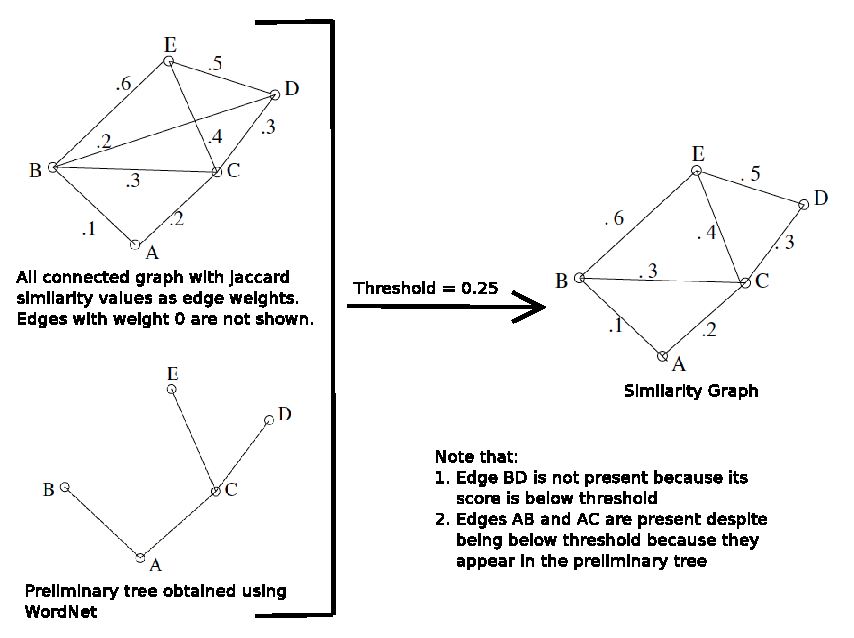
\includegraphics[width=0.8\linewidth]{TagTree/CreatingSimGraph}
\caption{Building the Similarity Graph for threshold $\tau$=0.25} 
\label{fig:sim}
\end{figure}
%\subsection{Objective Function} \label{subsec:objfunction}
Given the similarity graph $\mathcal{G_T}$, the objective of the refinement stage is to find a tree in the space of spanning trees of the similarity graph $\mathcal{G_T}$ which minimizes a defined objective function. Below we define and motivate two different objective functions based on corpus statistics, for tag tree construction. 
\begin{enumerate}
\item \textbf{Weighted Average Hops (WAH)}: 
\begin{equation}
\; \sum_i\sum_{j, j < i}{J_{\mathcal{T}}(i,j)d_{i,j}} , 
\label{eq:ObjFnWeightedHops}
\end{equation}
where $d_{i,j}$ represents the number of hops between tag $t_i$ and tag $t_j$ in the tag tree. The motivation for such a score is that it is lower when tags $i$ and $j$ with high $J_{\mathcal{T}}(i,j)$ are separated by fewer hops as compared to tags with low $J_{\mathcal{T}}(i,j)$. \hl{The above objective function is equal to the sum of the pair-wise hops between all pairs of tags weighted by the corresponding Jaccard similarity {$J_{\mathcal{T}}(i,j)$}. Dividing the sum by 
$\sum_{i,j < i}{J_{\mathcal{T}}(i,j)}$ would be equal to the weighted average number of pair-wise hops where the weights are normalized Jaccard similarities. Since the value $\sum_{i,j <  i} {J_{\mathcal{T}}(i,j)}$ is a constant for a given set of tags {$\mathcal{T}$}, we have removed the scaling factor from the objective function. }
For a general graph $\mathcal{G_T}$, the problem of minimizing the weighted average number of hops has been established to be an NP hard problem \cite{garey1979computers}.  
\item \textbf{Similarity Approximation (SA)}: 
\begin{equation}
\; \sum_i\sum_{j, j < i}{w_{i,j}\mid J_{\mathcal{T}}(i,j) - S_T{(i,j)}} \mid  , \\
\label{eq:ObjFnSimApprox}
\end{equation}
where $S_T{(i,j)}$ represents the similarity between tags $t_i$ and $t_j$ estimated using tag tree $T$. A very close problem is that of approximating a given distance matrix through spanning trees, which has been established to be NP hard~\cite{eckhardt2005combinatorial}. The objective function in~(\ref{eq:ObjFnSimApprox}) is the weighted L1 norm of the difference between the Jaccard Matrix $J_{\mathcal{T}}$ and the \textbf{Estimated Similarity Matrix} $S_T$. \hl{The weights $w_{i,j}$ are taken to be the co-occurrence counts of tags $t_i$ and $t_j$ and are useful to establish relative importances between different pairs of tags in the objective function}. While $S_T{(i,j)}$ can be calculated in several ways for a given tag tree $T$, we define $S_T{(i,j)}$  as 
\begin{equation}
S_T{(i,j)} = \prod_{e \in \mathfrak{P}_{i,j}}{S(e)}  , \\
\label{eq:ProdSimSimilarityCalculate}
\end{equation}
where $\mathfrak{P}_{i,j}$ is the path in tag tree $T$ connecting tags $t_i$ and $t_j$ and $S(e)$ is equal to the Jaccard similarity between the tags that edge $e$ connects. Such a definition for $S_T{(i,j)}$  ensures that it lies between 0 and 1 and no rescaling is required in order to compare $S_T{(i,j)}$  values with $J_{\mathcal{T}}(i,j)$.
\end{enumerate}
\hl{Note that the trees in ({\ref{eq:ObjFnWeightedHops}}) and ({\ref{eq:ObjFnSimApprox}}) are constrained to be spanning trees over the Similarity Graph $\mathcal{G_T}$. }The local search based approach to minimize either of the above objective functions is described next. 
\vspace{-0.12in}
\subsection{Optimization based on Local Search}
\label{subsec:localsearch}
\comment{
\noindent In this section we describe the construction of the tree. We split this process into the following two steps:
\begin{enumerate}
%\item {\bf {\em Constructing a similarity graph}}: We define a similarity metric for each pair of tags and threshold it appropriately to obtain a binary feature. i.e. we will call a tag pair {\bf {\em ``similar''}} iff their similarity score is greater than a threshold $t$. This is then used to build a similarity graph $\mathcal{G_t}$ where the vertices correspond to the tags and the edges correspond to tag pairs that are similar.
\item {\bf {\em Constructing a similarity graph}}: We start with the tree on the set of tags built using the WordNet database. We define a similarity metric for each pair of tags and threshold it appropriately to obtain a binary relation. i.e. we will call a tag pair {\bf {\em ``similar''}} iff their similarity score is greater than a threshold $t$. We then add the edges corresponding to similar tag pairs to the original tree and obtain the similarity graph which we will denote by $\mathcal{G_t}$.
\item {\bf {\em Building an optimized tree}}: On the set $\mathcal{S}$ of spanning trees of $\mathcal{G_t}$, we define a neighbour relation and a potential function and find a minimal tree using the local search paradigm.
\end{enumerate}

\subsection{Similarity Graph}

***** TODO (Chetan) ***** \\
--Fill in details of how initial tree using WordNet is constructed \\
********* \\



*****  TO BE FILLED **************** \\
-- Describe the threshold and the distribution from which it is calculated \\
--  We can't say $t$ is empirically estimated as mean $J(s_1, s_2)$ because that might make spanning trees infeasible \\
******************************************
}
Given the Similarity Graph $\mathcal{G_T}$ for a set of tags $\mathcal{T}$, our objective is to construct a spanning tree on $\mathcal{G_T}$ such that the defined objective function is minimized. Since finding spanning trees of $\mathcal{G_T}$ that optimally minimize either (\ref{eq:ObjFnWeightedHops}) or (\ref{eq:ObjFnSimApprox}) is a hard problem, we propose an approach to obtain local optimum through the local search paradigm. 
\\
\indent \textit{Local Search} -- Local search algorithms provide a local optimum to an optimization problem. This is done by moving from one solution to another, in the search space of candidate solutions. \\
For the problem of constructing a ontological tag tree, we define a simple edge-exchange based  neighborhood on the space of spanning trees of the graph $\mathcal{G_T}$ as follows. Given two spanning trees $T_1$, $T_2$ we say that $T_2$ is a neighbour of $T_1$ iff it can be obtained from $T_1$ by the following process:
\begin{enumerate}
	\item Pick an edge $e_1 \in \mathcal{G_T}\setminus T_1$ and add it to $T_1$. 
	\item In the (unique) cycle thus formed in $T_1$ containing $e_1$ pick the edge, say $e_2$ with minimum weight (i.e., jaccard similarity of the tags $e_2$ connects). Remove $e_2$ from $T_1$. 
\end{enumerate}
Starting from a spanning tree $T_0$ of $\mathcal{G_T}$ as an initial solution, we explore all neighbors of $T_0$ to determine which neighbor minimizes the defined objective function. The winning neighbor is then considered as the next solution and its neighbors are explored until no further benefit is seen in the objective function. The steps of the local search based ontological tree construction are listed in Algorithm~\ref{algo:STCAlgorithm}. The output is the locally optimal tag tree $T_{opt}$. Note that $T_0$ is taken as $T_W$ as obtained from Algorithm~\ref{alg:WordNetSTAlgo}. Fig.~\ref{fig:neighborhood} show one iteration of the proposed local search based approach for the objective function in (\ref{eq:ObjFnWeightedHops}). 
\begin{algorithm}
\fontsize{8pt}{1em}\selectfont
\caption{Ontological Tree Construction Algorithm}
\label{algo:STCAlgorithm} 
\textbf{Input:} \\
$\cdot$ Similarity graph $\mathcal{G_T}$ for a given set of tags $\mathcal{T}$ \\ 
$\cdot$ Initial Solution: $T_0$. \\
$\cdot$ \hl{Pair-wise Jaccard similarities between tags, i.e., $J_{\mathcal{T}}(i,j)$}
\textbf{Initialization:} 
$S$=$T_0$ \\
%$T_0$ can be randomly selected as any spanning tree over $\mathcal{G_T}$, or be picked in a heuristical manner \\
\textbf{Loop: } \\
\hspace*{5mm} $\cdot$ $E_{Candidates}$ := set of edges present in $\mathcal{G_T}$ and not in $S$ 
\hspace*{5mm} \textbf{For each edge $e$ in $E_{Candidates}$} \\
%\hspace*{10mm} (Exploring neighbors of current solution)  \\
\hspace*{10mm} $\cdot$ Add edge $e$ in $S$ to get graph $G$. \\
\hspace*{10mm} $\cdot$ $E_{Cycles}$ :=set of edges in the cycle formed in $G$. \\
\hspace*{10mm} $\cdot$ Remove edge $e'$ with lowest weight (i.e., jaccard \\
\hspace*{10mm} \; similarity of connecting tags) from $E_{Cycles}$: $e' \neq e$ \\
\hspace*{10mm} $\cdot$ $S_{Neighbor}$ = spanning tree thus formed  \\
\hspace*{10mm} $\cdot$ Calculate objective function at $S_{Neighbor}$ \\
\hspace*{5mm} \textbf{EndFor} \\
\hspace*{5mm} $\cdot$ Select neighbor giving best objective function as $S_{Next}$ \\
\hspace*{5mm} $\cdot$ If $S_{Next}$ improves objective function over $S$ \\
\hspace*{10mm} $S=S_{Next}$ \\
\hspace*{5mm} $\cdot$ Else Stop iterating \\ 
\textbf{End Loop}. \textbf{Output:} locally optimal spanning tree $T_{opt}=S$
\end{algorithm}

\begin{figure}[htbp]
\begin{center}
\centering
%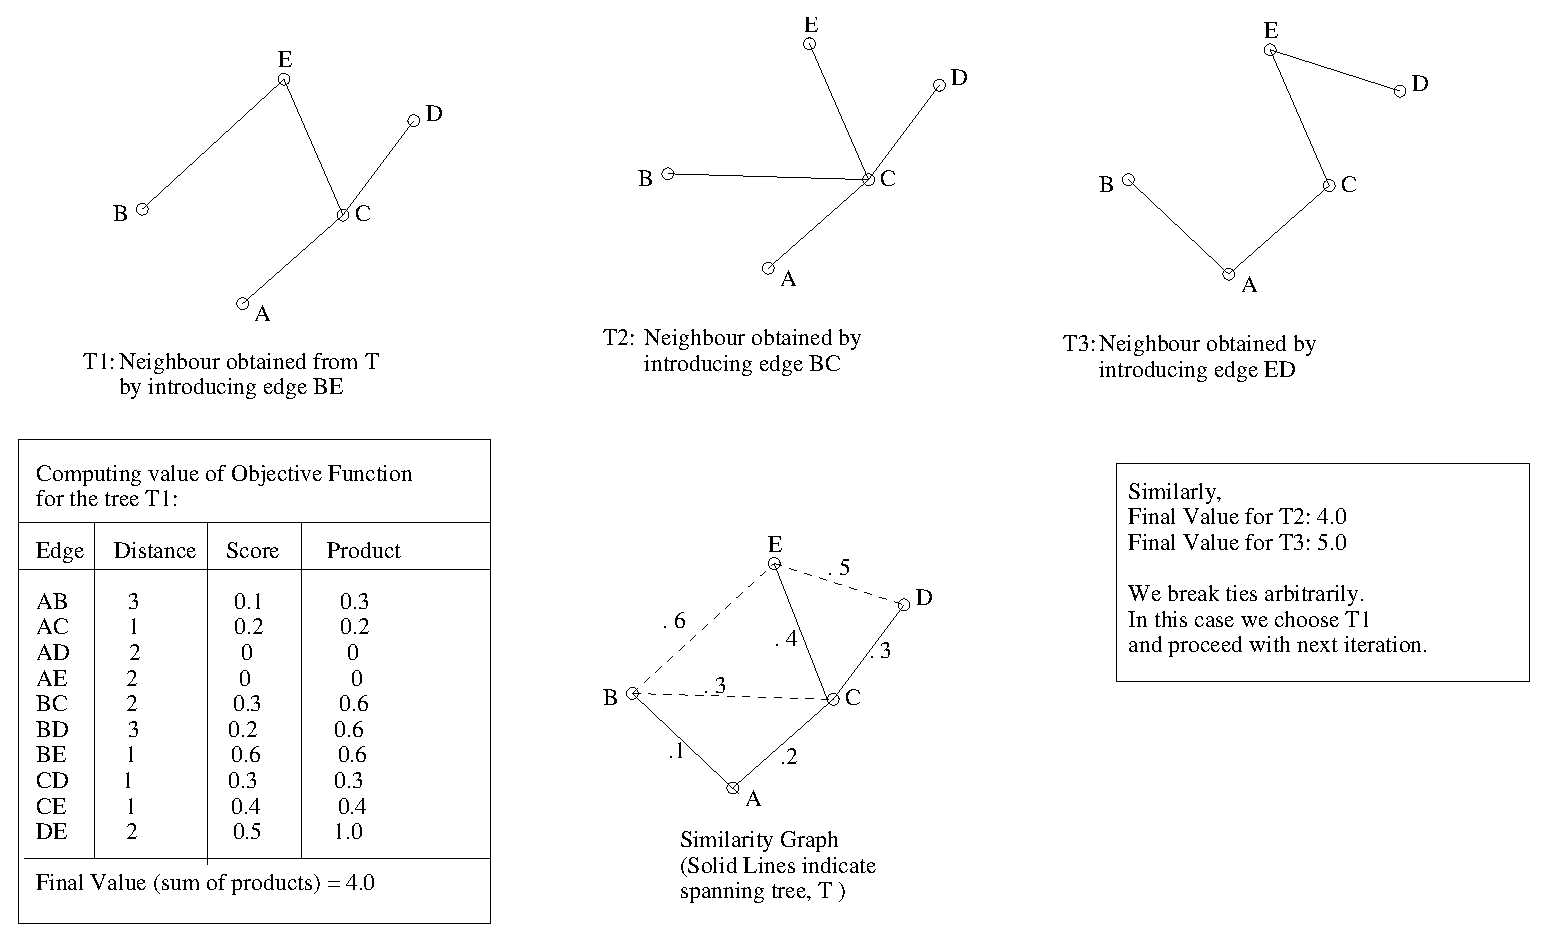
\includegraphics[width=0.8\linewidth]{Neighbourhood-2}
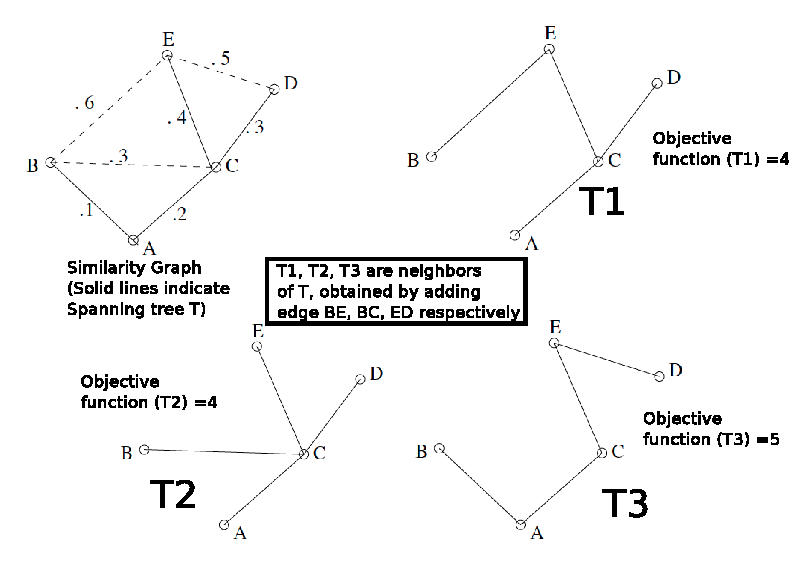
\includegraphics[width=0.8\linewidth]{TagTree/LSOneiteration}
\caption{One iteration of the proposed approach. Eq. (\ref{eq:ObjFnWeightedHops}) is utilized to calculate the objective function for neighbors of a tree T. Ties are broken arbitrarily. Since both T1 and T2 have an objective function~(\ref{eq:ObjFnWeightedHops}) value of 4, we choose T1 and proceed to next iteration. } 
\label{fig:neighborhood}
\end{center}
\end{figure}
% \subsubsection{Optimization Function} 
% \subsubsection{Local Search}
\subsection{Effect of initializing using WordNet}
\comment{
\hl{Utilizing a preliminary tag tree that is constructed using the semantics obtained WordNet has two benefits. Firstly, this biases the constructed structure to have connections dictated by semantic similarity when the data driven relations between certain tags are not strong enough to uniquely determine the structure of the tag tree. The constructed tag tree would thus have edges that are explicable based on the semantic similarity of the tags, as compared to randomness induced as an artefact of the construction procedure. As compared to other tag trees with possibly similar value of the objective function, the resulting tag trees offer a clean interpretation of the relationship between the tags. For example, consider four tags A, B, C, D with pair-wise jaccard similarities as given in Fig. {\ref{fig:ExampleWhyWordnet}}. 
}
\comment{
\begin{table}[htbp]
\scriptsize
\begin{center}
\caption{\hl{Example pair-wise jaccard similarities}}
\label{tab:ExampleWhyWordnet}
%\begin{tabular}{|p{4cm}|p{3.0cm}|}
\begin{tabular}{|c|c|c|c|c|}
		\hline
		 & A & B & C & D \\ 
		\hline 
		A & 1 & 0.9 & 0.1 & 0.3 \\ 
		\hline 
		 B & 0.9 & 1 & 0.2 & 0.2 \\ 
		\hline
		 C & 0.1 & 0.2 & 1 & 0.2 \\
		\hline
		D & 0.3 & 0.2 & 0.2 & 1 \\
		\hline 
\end{tabular}
\end{center}
\end{table}
}
\hl{Based on the first (LS-WAH) objective function ({\ref{eq:ObjFnWeightedHops}}), the two tag trees that would have the same value of the objective function (equal to 2.5) are shown in Fig.~{\ref{fig:whywordnet}} as X and Y. The tag tree as per WordNet is denoted by W. Random initializations of the local search based optimization as detailed in Section {\ref{sec:ConstructionTree}} can lead to either of X or Y as the solution. However initializing using W leads to a unique solution Y where tag B is connected to tags C and D, as in W, thus preferring connections that conform to their semantic relationship. \\
\textbf{Question: Should we even have the first para and its figs?\\ }
} }
\hl{The benefit of using WordNet to initialize the proposed local search based approach is that as compared to random initializations, the former helps achieve a preferred value of the objective function faster. The typical way to attain a lower value of the objective function for an optimization problem as defined in Section {\ref{sec:refinement}} would be to run the local search using randomly constructed tree on the set of tags as initialization, and picking the best tree across several such runs based on the tag tree that has lowest objective function. However this requires running the local search several times which can be large considering that the number of spanning trees on a set of $N$ tags varies as $N^{N-2}$~{\cite{cayley1894collected}}. The preliminary tree as constructed using WordNet offers a more meaningful initialization to the local search by capturing certain types of relationships between the tags that are dictated by their semantics. Table {\ref{tab:WordNetRandominitGWS30}} provides the statistics of the objective function of tag trees constructed by running the proposed local search based approach 20 times with random initializations. As can be seen, a single run using WordNet based preliminary tag tree leads to a much better objective function~({\ref{eq:ObjFnSimApprox}}). Also, the resulting tag tree using WordNet leads to a better performance than the best across 20 runs with random initializations. Note that for Table {\ref{tab:WordNetRandominitGWS30}}, the performance of tag trees is measured using Average Tag Prediction Accuracy as discussed in Section {\ref{sec:Expts}}.} 

\comment{
\begin{figure}[h]
\begin{center}
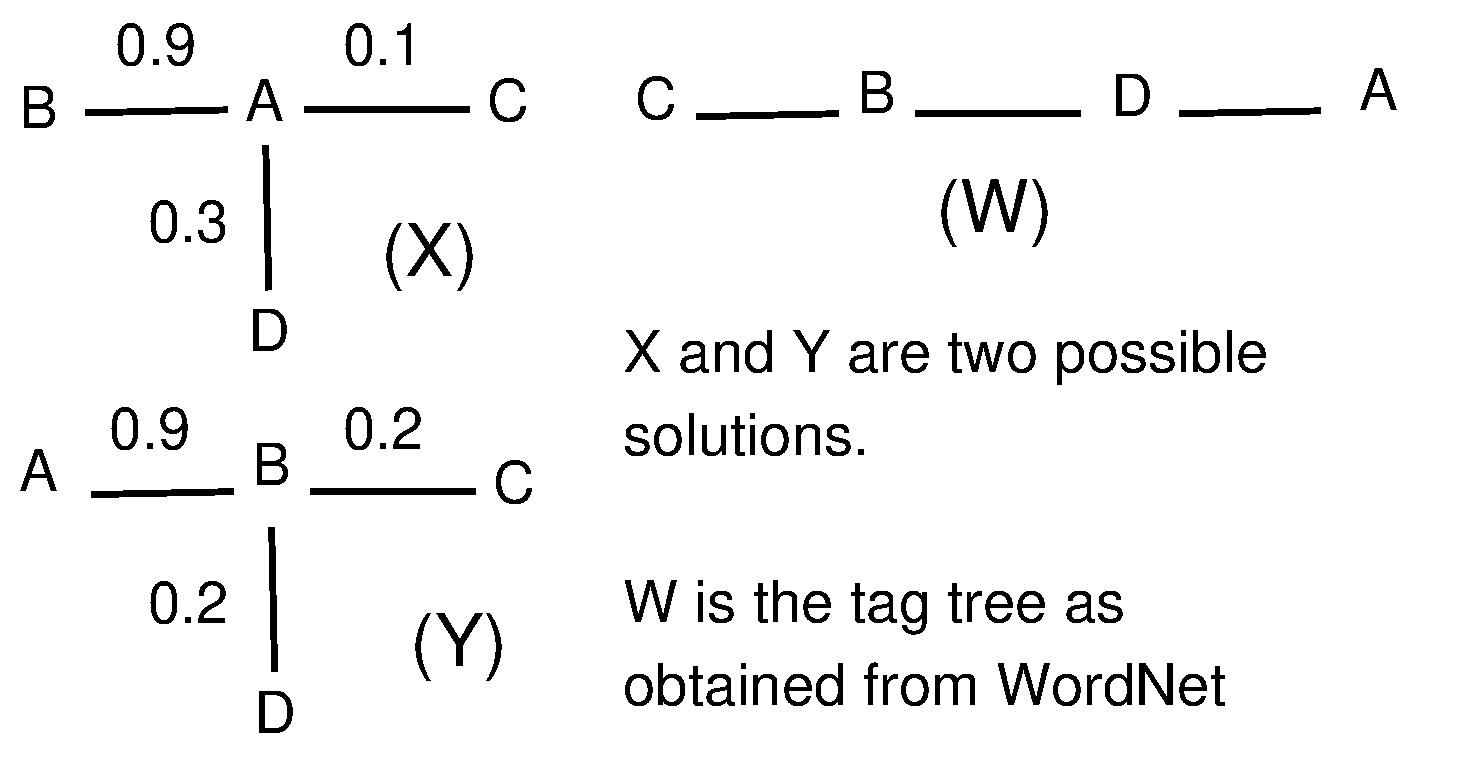
\includegraphics[width=0.65\linewidth]{TagTree/WhyWordNetExample}
\caption{\hl{Example showing multiple solutions using (LS-WAH) objective function ({\ref{eq:ObjFnWeightedHops}}) } }
\label{fig:whywordnet}
\end{center} 
\end{figure}
}
\comment{
\begin{figure}[t!]
\centering
\minipage{0.17\textwidth}
%\centering
  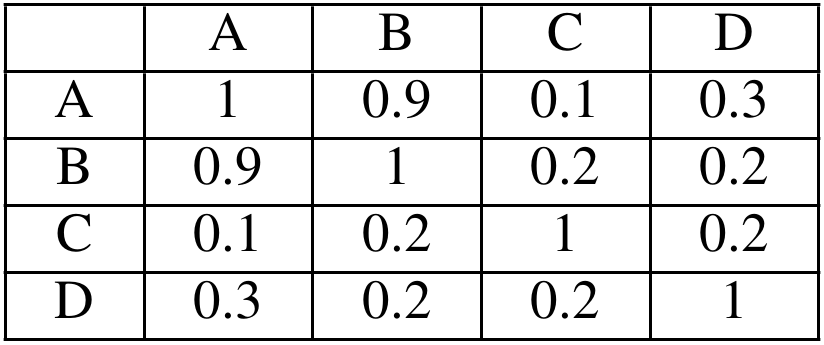
\includegraphics[width=\linewidth]{TagTree/TableWordNetExample.png} 
\caption{\hl{Example pair-wise jaccard similarities}}
\label{fig:ExampleWhyWordnet}
%\end{centering}
\endminipage %\hfill
\hspace{0.1in}
\minipage{0.28\textwidth}
  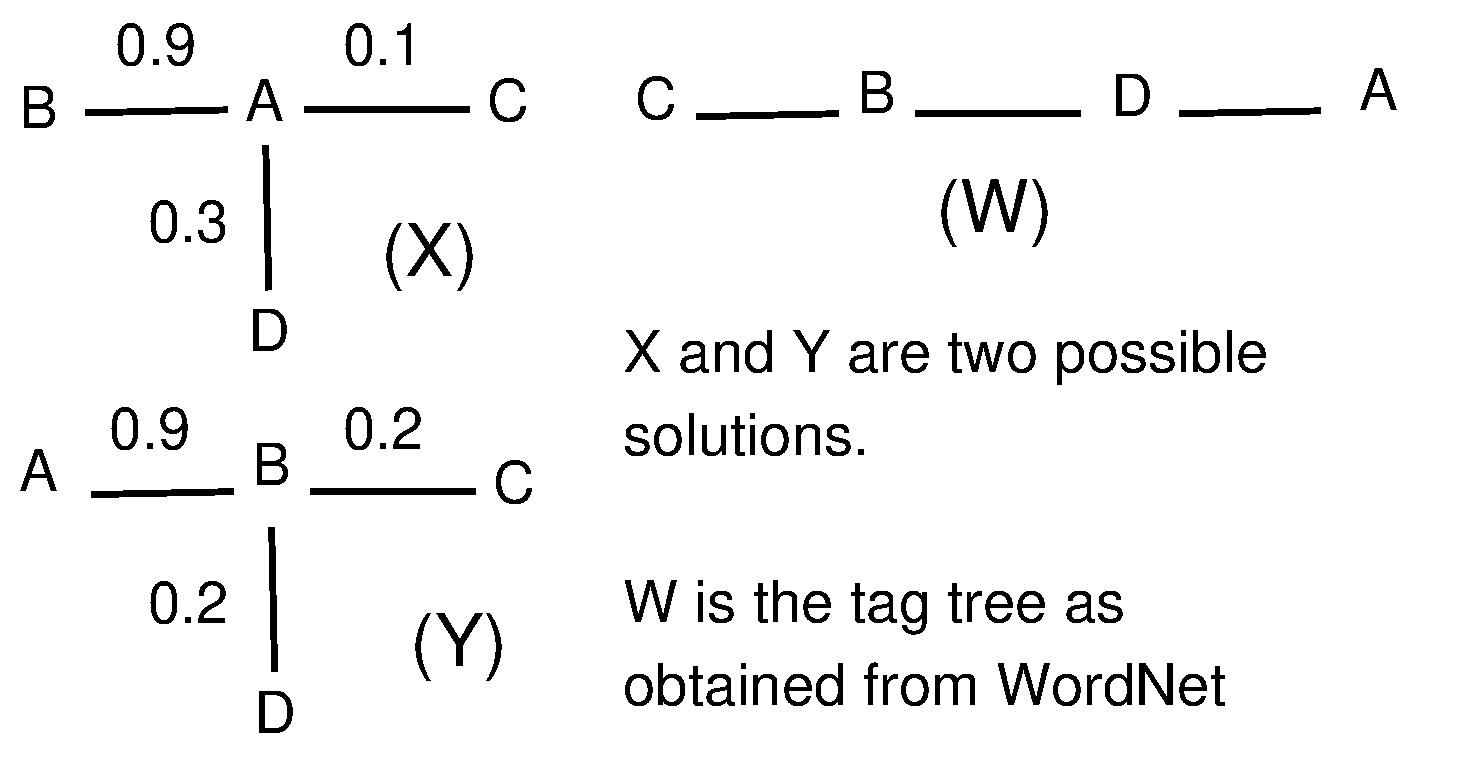
\includegraphics[width=\linewidth]{TagTree/WhyWordNetExample}
\caption{\hl{Example showing multiple solutions using (LS-WAH) objective function ({\ref{eq:ObjFnWeightedHops}}) } }
\label{fig:whywordnet}
\endminipage %\hfill
\end{figure}
}
\begin{table}[htbp]
%\scriptsize
\begin{center}
\caption{Effect of initializing the proposed local search based approach using WordNet. 30 tags from stock image corpus (described in Section IV) are used. }
\label{tab:WordNetRandominitGWS30}
\begin{tabular}{lllll}
\toprule 
     & \multicolumn{3}{c}{Random initialization} & \multicolumn{1}{c}{Using WordNet}\\

    & Min & Mean & Max & \multicolumn{1}{c}{}  \\
    \midrule
    Objective function ((4) x $10^6$) & 6.4    & 13.7  &  47.7  & \multicolumn{1}{c}{0.6} \\
    Performance (in \%) & 24.2    &43.8  & 49.2  & \multicolumn{1}{c}{50.9} \\
    \bottomrule
\end{tabular}
\end{center}
\end{table}
\section{Evaluation} 
\label{sec:Expts}
In this section, we describe the experimental setup for the construction and evaluation of ontological tag trees. For the evaluation, we define tag prediction and efficient classification tasks as discussed later in this section. The experiments are conducted on two large corpora of images, the details of which are given below.  
\vspace{-0.1in}
\subsection{Datasets} 
\label{sec:Datasets}
To test the robustness of our approach to build ontological tag trees for domains with varying degrees of tag noise, we use two different image corpora - one from Flickr, composed primarily of user generated content, and one from a professionally curated stock photo agency.
\begin{itemize} 
\item \textbf{Flickr images}: Flickr~\cite{Flickr} is a popular image and video hosting website where users can upload images and associate them with annotations such as titles, tags and descriptions, among others. As Flickr primarily contains user generated content, tags are often noisy, irrelevant to image content or even completely absent. 
%As can be seen in Fig.~\ref{fig:CDFFlickr}, more than 90\% Flickr images have 13 or less tags associated with them. 
We utilize 500,000 images for training and 100,000 images for testing. All these images are licensed under Creative Commons copyright licenses.
\item \textbf{Stock images corpus}: To evaluate the proposed approach on less noisy data, we take a corpus of stock photos that are professionally annotated, and hence are accompanied with a variety of accurate annotations - such as keywords, captions, etc. For this corpus, we use the set of keywords to build the ontological tag tree, and refer to them as "tags".
%Images are professionally annotated and hence 90\% of Getty images have 38 or less tags (Fig.~\ref{fig:CDFGetty}), which is much more than in the case of Flickr. 
We utilize more than 350,000 images for training and close to 70,000 images for testing. The textual captions are used in the efficient classification task as shown in Section~\ref{sec:effClassification}.
\end{itemize} 

Training images are used for adapting the WordNet based preliminary tag tree obtained using Algorithm~\ref{alg:WordNetSTAlgo} to the given corpus using the local search based approach described in Algorithm~\ref{algo:STCAlgorithm}. Training images are also used for specific required tasks such as training of classifiers. Testing images are used to evaluate the constructed tag trees. There is no overlap between training and test sets.



\subsection{Effect of Local Search based Optimization}
We first demonstrate how the proposed local search based approach helps in improving the objective function as defined in Section~\ref{sec:ConstructionTree}. Fig.~\ref{fig:ObjFun} shows the variation of the objective function in (\ref{eq:ObjFnWeightedHops}) with the number of iterations on Flickr tag corpus. The objective function value of the WordNet based preliminary tag tree for Flickr corpus before the proposed refinement is $357.2$ that becomes $167.1$ using the local search based refinement in $68$ iterations. Median of the Jaccard similarity values is taken as the threshold $\tau$ for candidate selection in the proposed refinement algorithm. Similar improvement is observed for the Stock images corpus, for which the objective function values improves from $224.5$ to $99$ after 23 iterations. For both corpora, the iterations are terminated once no further improvement is observed in the objective function. We describe below the tasks defined to evaluate the constructed tag trees. 
\begin{figure}[h!]
\begin{center}
%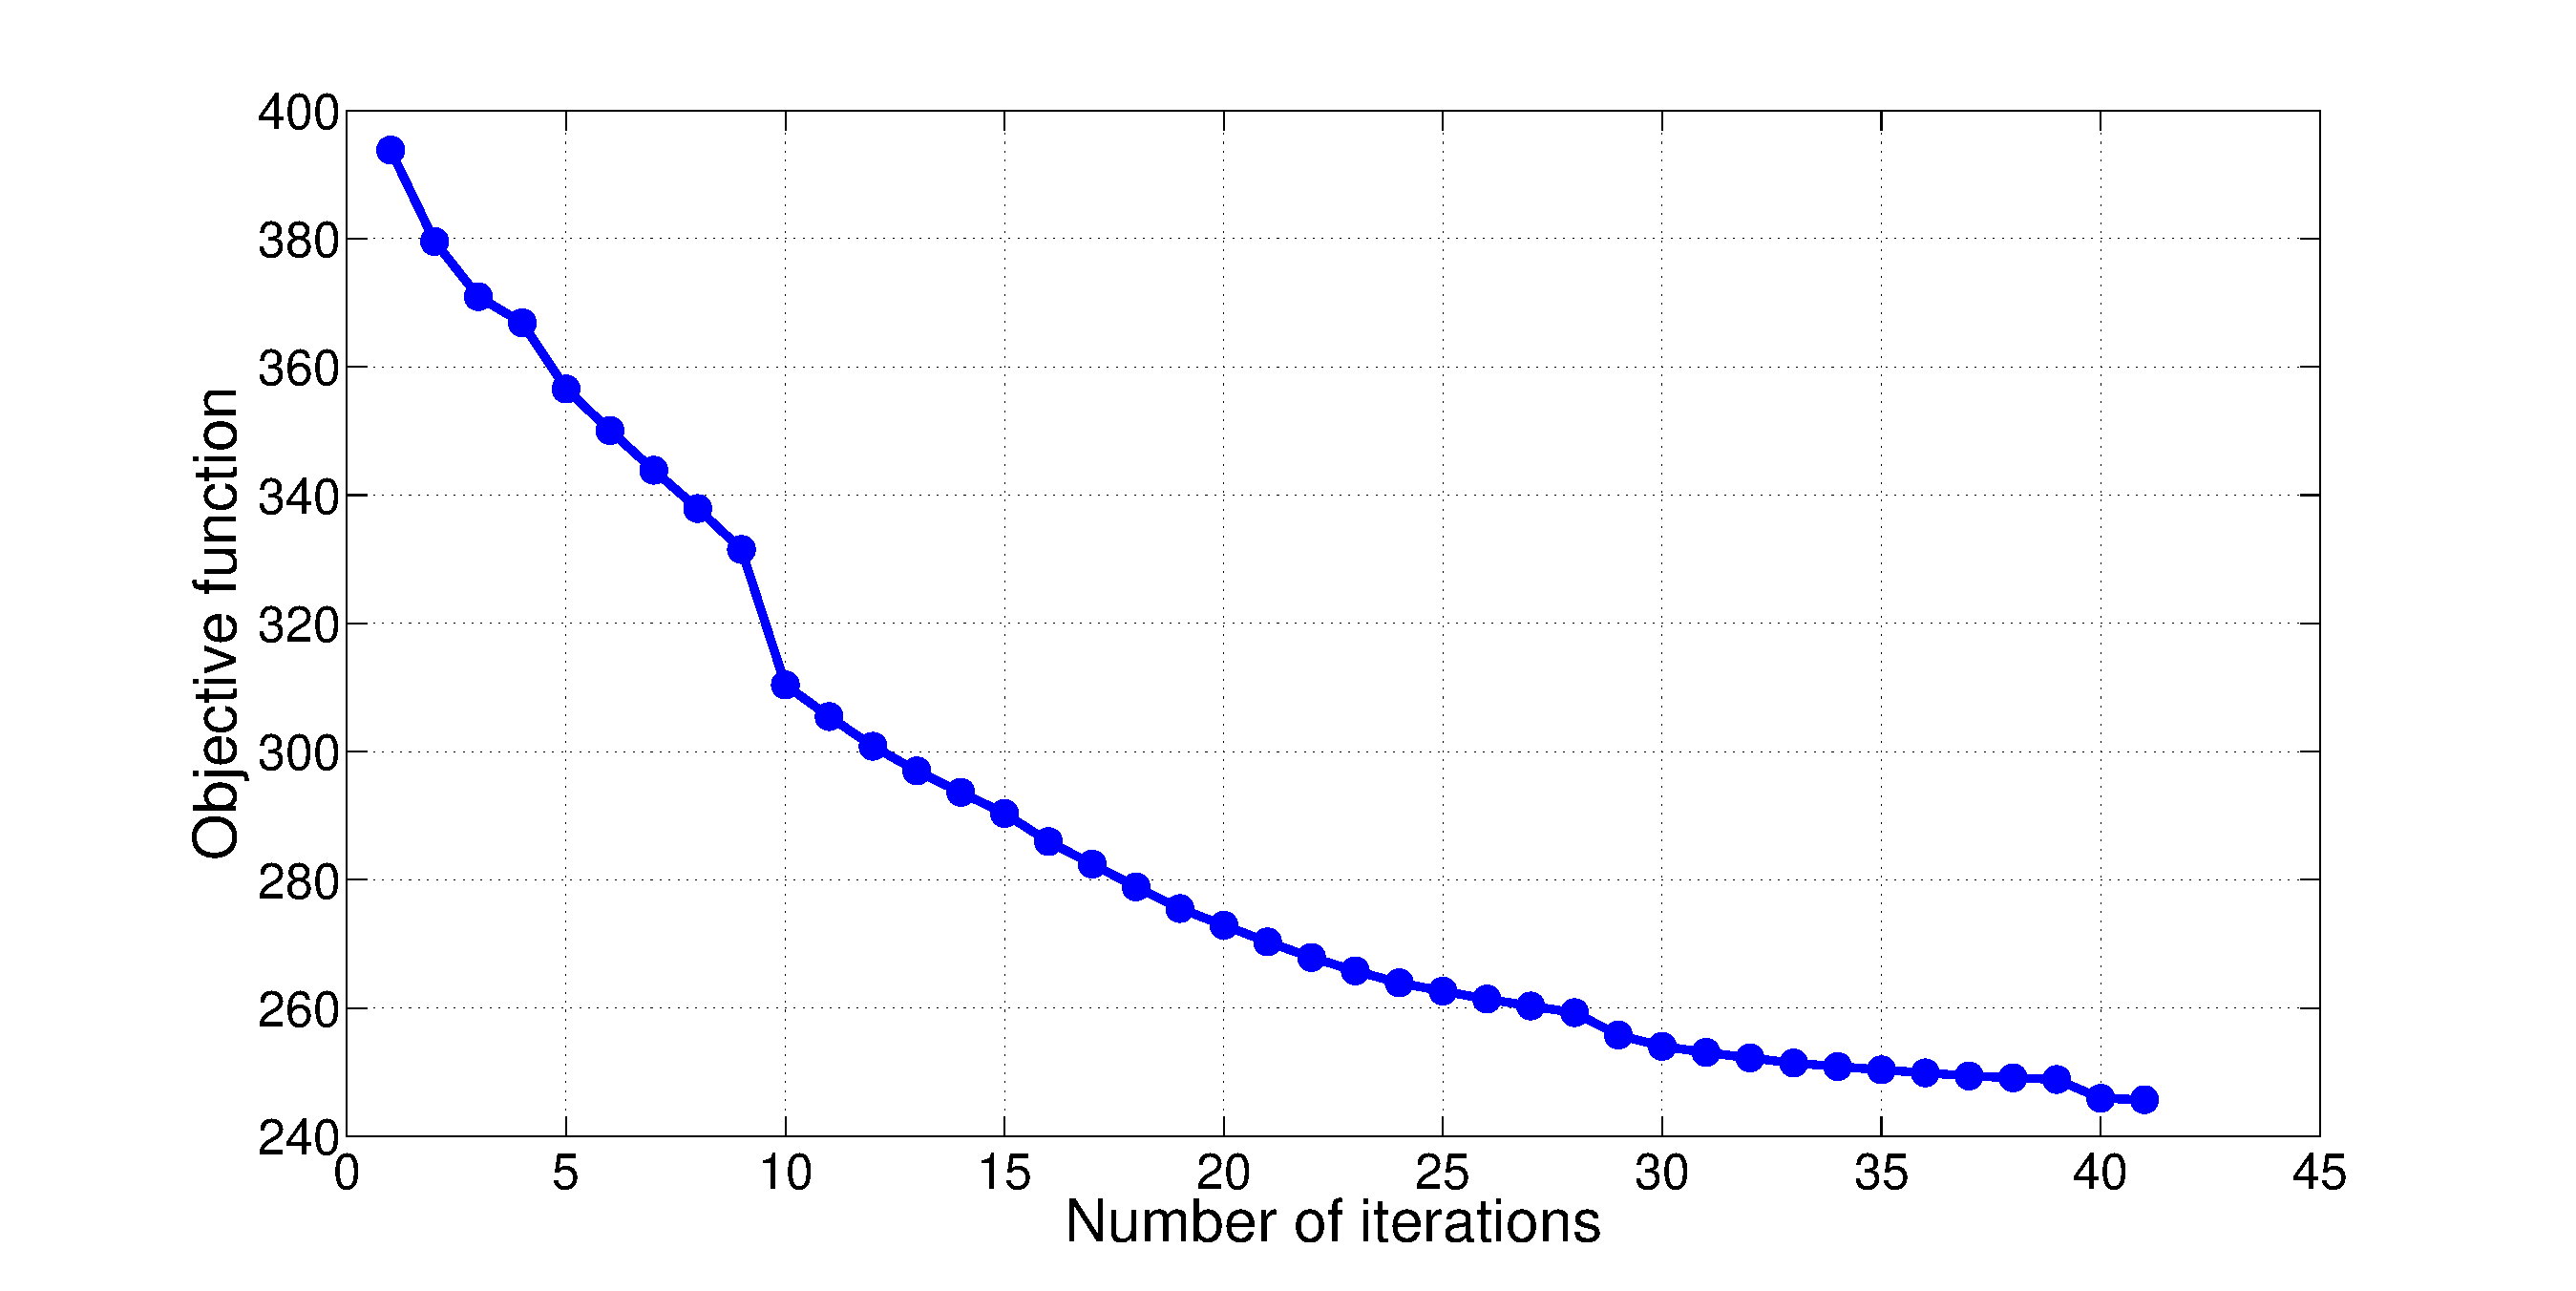
\includegraphics[width=0.8\linewidth]{TagTree/SigmaCijDijVariatPerIter999point05STGD}
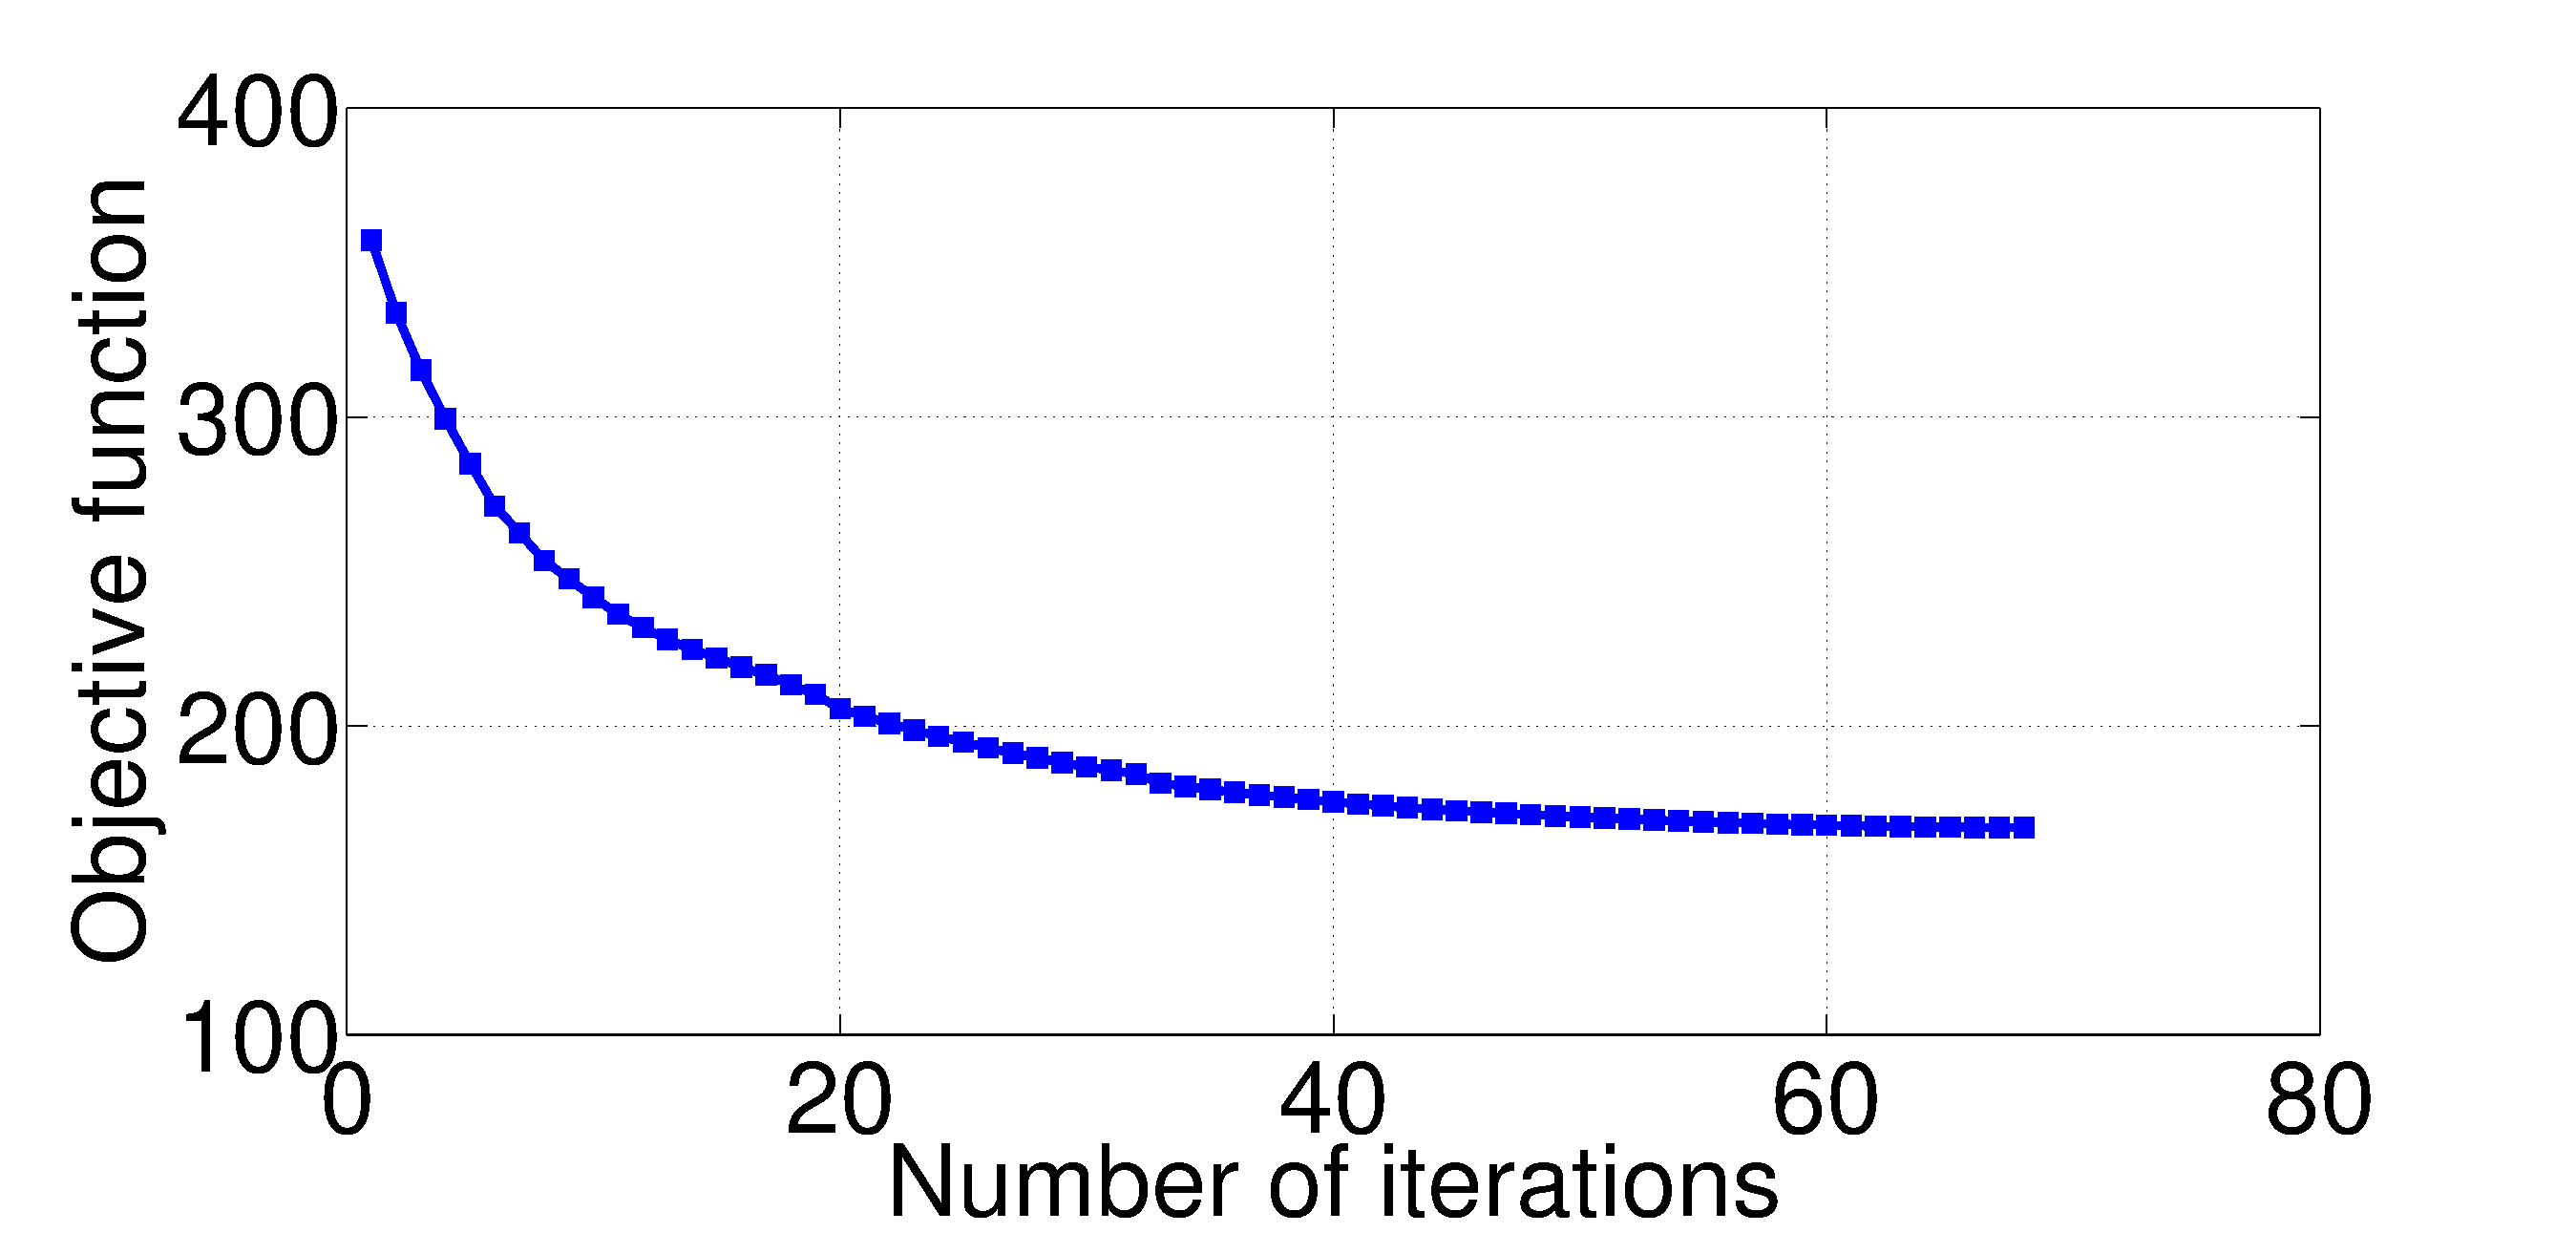
\includegraphics[width=0.65\linewidth]{TagTree/LSWWW_objectivefnValuePerIteration}
\caption{The variation of the objective function~(\ref{eq:ObjFnWeightedHops}) with the number of iterations for a sample run on Flickr tag corpus.} 
\label{fig:ObjFun}
\end{center}
\end{figure}
%We describe below the tasks defined to evaluate the constructed tag trees. 
% \indent \textit{Subsumption-based Semantic Graph} - \cite{SubsumptionText} and \cite{SubsumptionFlickr} utilize a rule-based subsumption model to derive hierarchies from text corpus and Flickr respectively. We utilize the same model to construct hierarchy for keywords of interest, and construct semantic graph by disregarding parent-child relationships and keeping only the edges. \\ 
% \indent We evaluate the performance of a semantic graph by utilizing the graph to assist in classification as detailed below. 
\subsection{Tag Prediction Task} 
\label{subsec:TagPred}
%The intuition behind this task is that a semantic graph that provides better performance in tag prediction is able to capture the information that characterizing the corpus in a much better manner. 
%Tag prediction is performed with the help of a given graph as detailed below. 
 
\hl{The tag prediction task is similar to the tag recommendation task in  {\cite{katsurai2013cross}} and in {\cite{sigurbjornsson2008flickr}}. However as outlined in Section {\ref{sub_sec:relatedWork}}, the proposed task does not require manual labeling for the resources (images) to evaluate the proposed tag tree construction approach. In order to do so, we divide the tags associated with a resource into a seen and an an unseen set of tags and use the latter to evaluate the predicted tags. We demonstrate this approach through experiments conducted on image corpora. 
}
Let an image $i$ in the corpus be tagged with the set of tags $\mathcal{T}_i$, such that $\mid \mathcal{T}_i \mid =N_{Tags}$. Assume that out of these $N_{Tags}$ tags, only a subset $\mathcal{T}_{i,Seen}$ are observed, with $\mid \mathcal{T}_{i,Seen} \mid=N_{Seen}$. The objective of the \emph{tag prediction task} is to predict the remaining ($N_{Tags} - N_{Seen}$) tags, i.e., $\mathcal{T}_i \setminus \mathcal{T}_{i,Seen}$.  Let $\mathbb{P}_i$ be the set of ($N_{Tags} - N_{Seen}$) tags predicted for image $i$ assuming that $\mathcal{T}_{i,Seen}$ is observed. Note that the prediction assumes the total number of tags for the image, $N_{Tags}$, to be known. Performance of tag prediction can be measured by the \emph{Tag Prediction Accuracy}, defined as follows: 
\begin{equation} \label{eq:TagPredAccuracy}
%\text{Tag Prediction Score} = \frac{\mid  \{\mathcal{T}_i \setminus  \mathcal{T}_{i,Seen}\} \cap \mathbb{P}_i \mid}{ \mid \{  \mathcal{T}_i \setminus  \mathcal{T}_{i,Seen} \}  \cup \mathbb{P}_i \mid} .
\text{Tag Prediction Accuracy} = \frac{\mid  \{\mathcal{T}_i \setminus  \mathcal{T}_{i,Seen}\} \cap \mathbb{P}_i \mid}{ \mid \{  \mathcal{T}_i \setminus  \mathcal{T}_{i,Seen} \} \mid} .
\end{equation} 

We now discuss the approach we follow to obtain the set of predicted tags $\mathbb{P}_i$ when the set of tags $\mathcal{T}_{i,Seen}$ is seen, by utilizing a given ontological tag tree. 
\subsubsection{Utilizing Ontological Tag Tree for Tag Prediction} 
\label{sec:TagPredUsingGraph}
Consider the tag tree $T$, built over the set of $\mathcal{T}$ tags in a corpus. For image $i$ with $N_{Seen}$ number of seen tags, each tag $t \in \{ \mathcal{T} \setminus \mathcal{T}_{i,Seen} \}$ is given a proximity score $s_t$ based on its proximity from the seen tags, as per $T$. Specifically, 
\begin{equation} 
s_t = \Sigma_{t' \in \mathcal{T}_{i,Seen} }{dist(t,t')}, 
\label{eq:TPEquation}
\end{equation}
where $dist(t,t')$ is the distance between tags $t$ and $t'$ in $T$ calculated as shown in Section~\ref{sec:comparison}. A lower proximity score for a tag $t$ indicates that it is closer in a cumulative sense to the set of observed tags $\mathcal{T}_{i,Seen}$. The tags are ordered in the increasing order of $s_t$, and the first ($N_{Tags} - N_{Seen}$) tags, i.e. those corresponding to the least values of $s_t$, are chosen as the set of predicted tags $\mathbb{P}_i$. \\

\subsubsection{Methods Compared} 
\label{sec:comparison}
We compare the following methods in the tag prediction task:
\begin{enumerate}
\item \underline{Random}: As the name suggests, this baseline method randomly picks  ($N_{Tags} - N_{Seen}$)  tags from the set $\mathcal{T} \setminus \mathcal{T}_{i,Seen}$. 

\item \underline{WordNet}: This baseline approach uses the semantics based ontological tag tree constructed from WordNet hierarchy using the procedure described in Algorithm 1. The edge weights are assigned to be semantic distances as obtained from \cite{RitaLibraryWordNet}. 
%\item \underline{(Weighted) WordNet hierarchy}: Same as the previous approach with the only difference being that semantic WordNet distances are used as edge weights instead of assigning them to $1$.
\item \underline{Google Similarity Distance}:  Google Similarity Distance \cite{cilibrasi2007google} has been used to construct tag graphs in applications such as tag ranking \cite{liu2009tag}. As mentioned in Section~\ref{sub_sec:relatedWork}, a threshold is used to discard certain edges in tag graphs. We choose a threshold such that for a tag graph with $N$ nodes (or tags), there are exactly $(N-1)$ edges remaining, so that the tag graph thus formed has same number of edges and space requirement as the tag tree learnt from proposed approach. Edge weights for the tag graph are taken to be the Google Similarity Distance as defined in \cite{cilibrasi2007google}. 

%In the approach, we obtain the tag graph based on the Google Distance model~\cite{SubsumptionFlickr}. In order to compare against the proposed approach, this is converted to an ontological graph by ignoring the directions and connecting the node with highest degree in each disconnected components, to a ``Root" node. The resulting subsumption graph is a spanning tree over the set of tags and an additional ``Root" node. 

\item \underline{LS Weighted Average Hops (LS-WAH)}:  Here we construct a tag tree using the proposed local search based approach, to minimize Weighted Average Hops (\ref{eq:ObjFnWeightedHops}) in Section~\ref{sec:refinement}. If an edge exists between tags $t_i$ and $t_j$ then the weight of the edge connecting them is given to be $(1-J_{\mathcal{T}}(i,j))$. 

\item \underline{LS Similarity Approximation (LS-SA)}:  This tag tree is constructed using the proposed approach with objective corresponding to Similarity Approximation as outlined in (\ref{eq:ObjFnSimApprox}) in Section~\ref{sec:refinement}. The edge weights are assigned as in Method 4 above. 

\item \underline{Symmetric sum based}: \hl{In order to compare the performance of the proposed tag tree construction approaches with that of other tag recommendation approaches that do not use tag trees or tag graphs or any visual features, we also provide the performance of the symmetric sum based approach as proposed in {\cite{sigurbjornsson2008flickr}}. Note that the space required to store the pair-wise similarities in {\cite{sigurbjornsson2008flickr}} is $O(N^2)$ while the proposed tag tree construction requires $O(N)$ space to store the tag tree. 
}


%For all present edges in the constructed tree, the weight of the edge is taken to be the jaccard similarity of the connecting tags. 

%\item \underline{LS on WordNet hierarchy}: This approach uses the refined ontological graph obtained using the proposed local search based algorithm (Algorithm 2). The edge weights are assigned to $1$ in this variant of the approach. 

%\item \underline{(Weighted) LS on WordNet hierarchy}: Same as the previous approach with the only difference being that inverse of Jaccard similarities are used as edge weights instead of assigning them to $1$.

\end{enumerate}
The prediction task is performed using the approach described in section~\ref{sec:TagPredUsingGraph}. For methods numbered 2, 3, and 4 above, $dist(t_i, t_j)$ as required in $(\ref{eq:TPEquation})$ is calculated by adding distances of edges in path connecting tags $t_i$ and $t_j$. For LS-SA method, $dist(t_i, t_j)$ is defined as $\{1- S_T{(i,j)}    \}$ where $S_T{(i,j)}$ is calculated for an ontological tag tree $T$ as per $(\ref{eq:ProdSimSimilarityCalculate})$. This is because the tag tree construction approach for LS-SA method utilizes product based similarity approximation $(\ref{eq:ProdSimSimilarityCalculate})$ and so it is appropriate to use same approach to estimate similarities based on a tree, and hence to calculate $dist(t_i, t_j)$. \hl{Similarly, for Symmetric sum based method {\cite{sigurbjornsson2008flickr}}, $dist(t_i, t_j)$ is defined as $\{1- J_{\mathcal{T}}(i,j)    \}$ where $J_{\mathcal{T}}(i,j)$ is the jaccard similarity between tag $t_i$ and $t_j$ as defined in Section~{\ref{sec:refinement}}. Note that this makes ({\ref{eq:TPEquation}}) similar to the sum based scoring approach in {\cite{sigurbjornsson2008flickr}}. 
}

%\indent The tag prediction task is conducted on two corpora, Flickr and the stock images corpus. We present the results in detail below. \\
\comment{
\begin{figure*}[!ht]
\minipage{0.32\textwidth}
  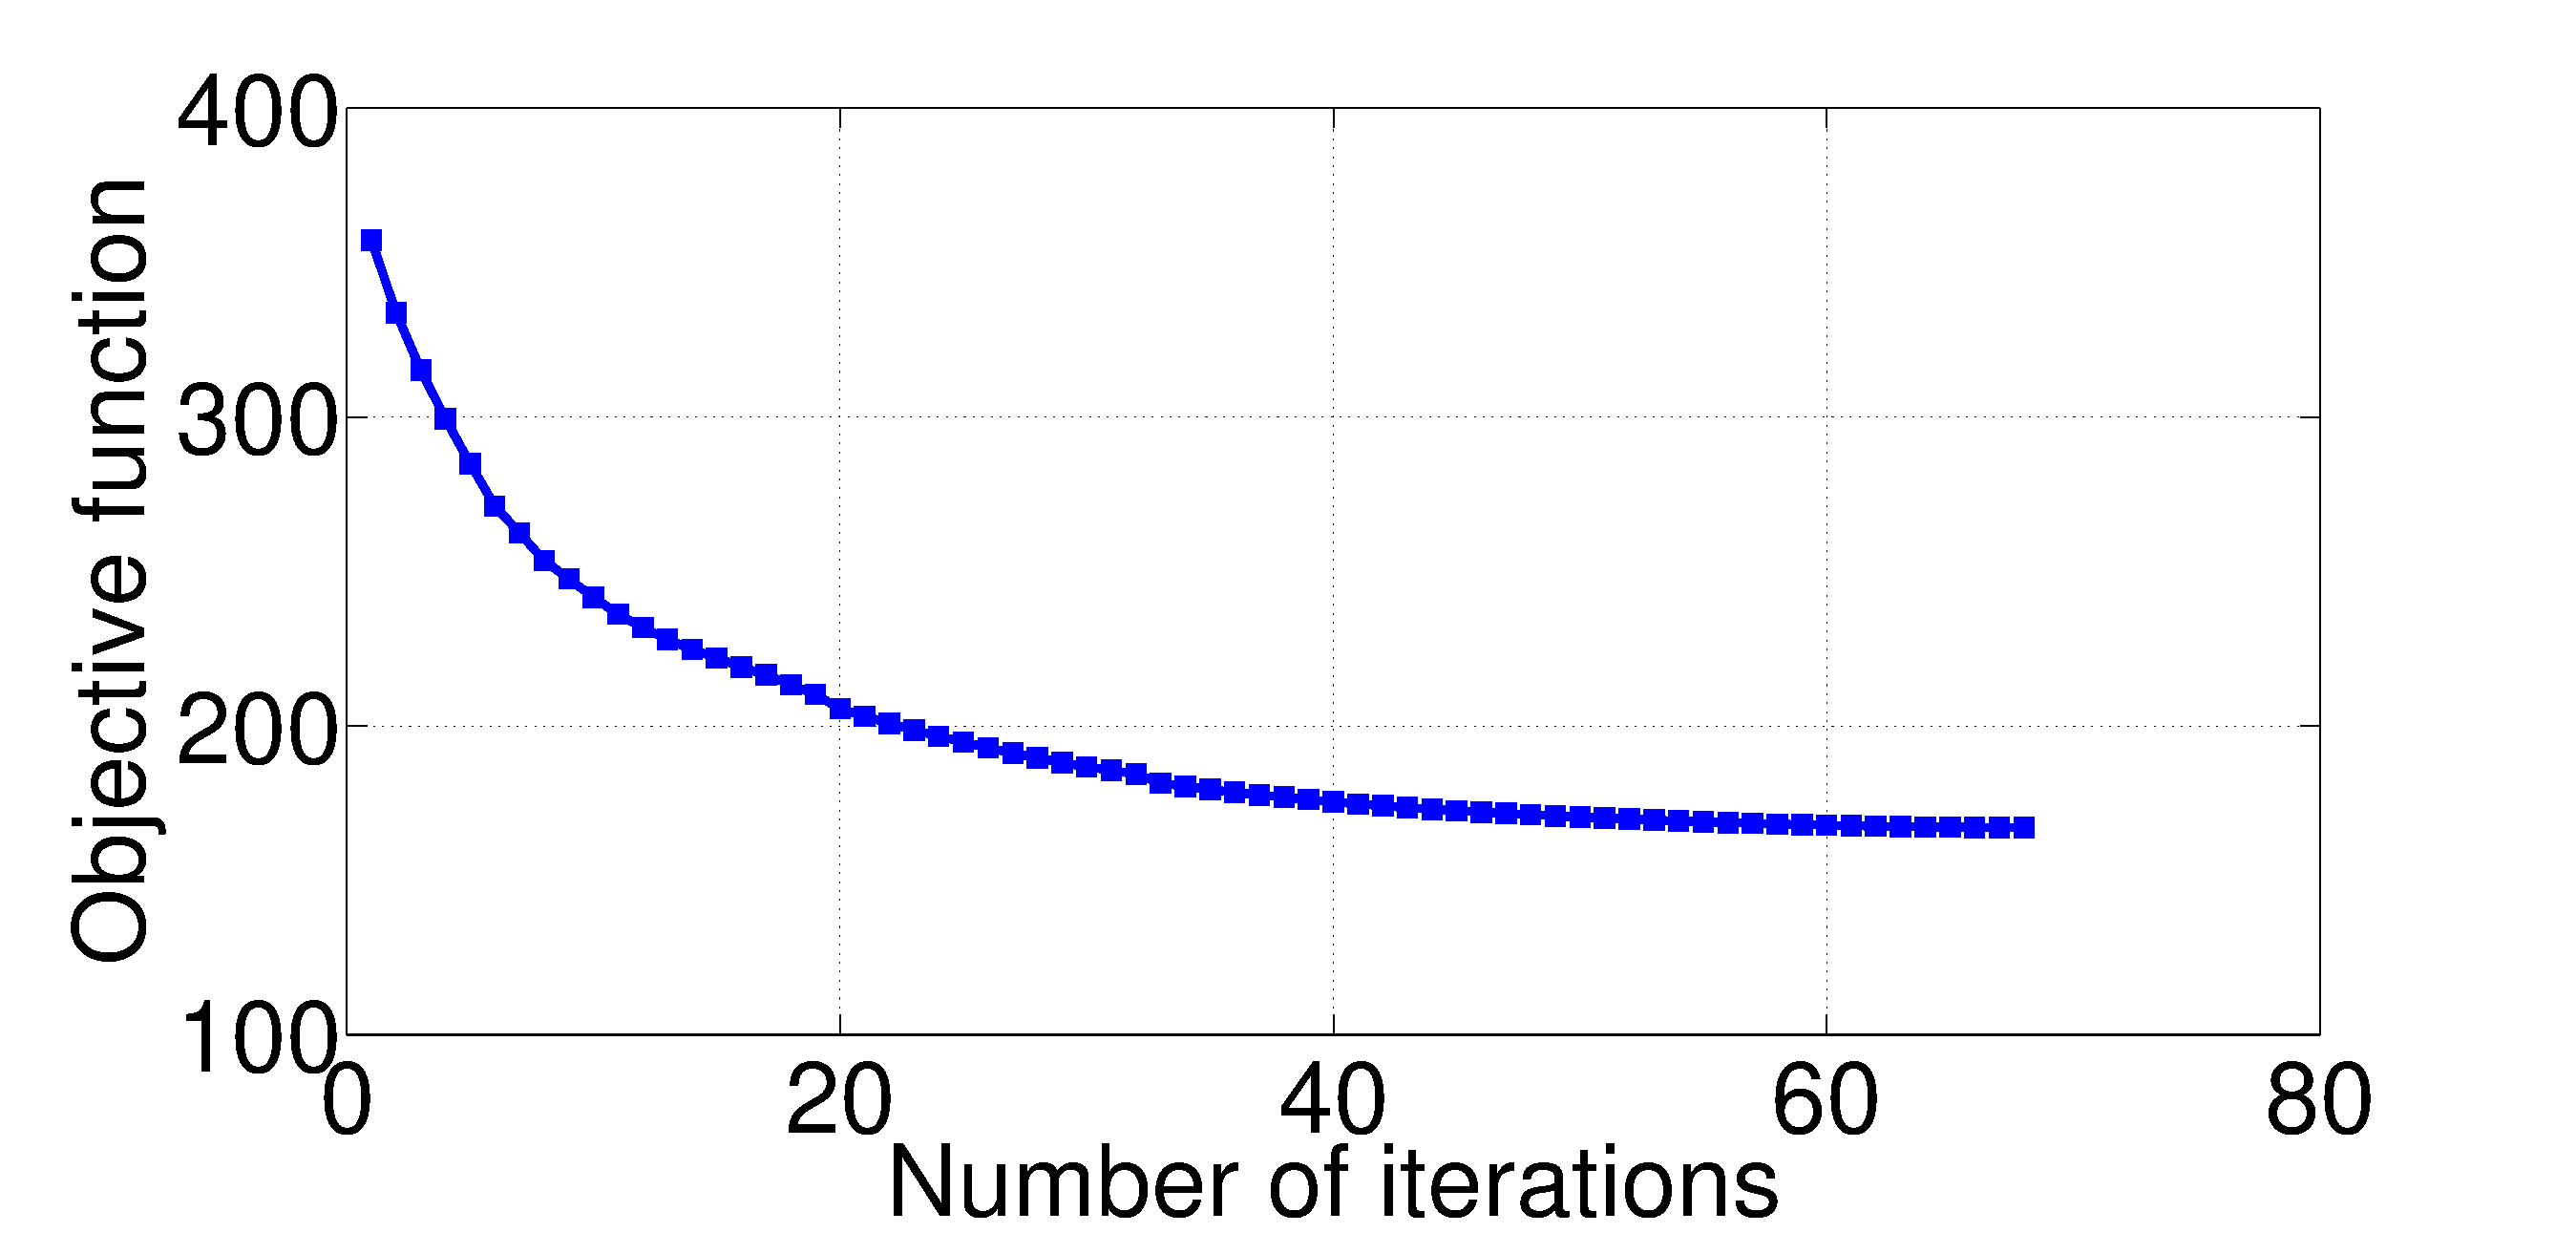
\includegraphics[width=\linewidth]{TagTree/LSWWW_objectivefnValuePerIteration}
\caption{The variation of the objective function~(\ref{eq:ObjFnWeightedHops}) with the number of iterations for a sample run on Flickr tag corpus.} 
\label{fig:ObjFun}
\endminipage\hfill
\minipage{0.32\textwidth}
  \includegraphics[width=\linewidth]{TPFlickr_rebuttal}
\caption{\hl{Average Tag Prediction Accuracies marginalized over $N_{Tags}$ for various methods for the tag prediction task on Flickr corpus. }} 
\label{fig:FWS117TagPredGraph}
\endminipage\hfill
\minipage{0.32\textwidth}%
  \includegraphics[width=\linewidth]{RebuttalGWS_TP}
\caption{\hl{Average Tag Prediction Accuracies marginalized over $N_{Tags}$ for various methods for the tag prediction task on Stock images corpus.}}
\label{fig:GWS30TagPredGraph}
\endminipage
\end{figure*}
}
\textbf{Flickr corpus:} We begin by choosing  the top $150$ most popular tags in a sample of Flickr images. After selecting only those tags that also occur in the WordNet database, we are left with 117 tags. These comprise the set $\mathcal{T}$. The total number of tags in an image, varies from 0 to 6 for most Flickr images. Since we need at least one tag to be seen and at least one to be predicted, we vary $N_{Tags}$  from 2 to 6. For each value of $N_{Tags}$, test images are selected which contain exactly $N_{Tags}$ tags. For each such image $i$, all combinations of $N_{Seen}$ tags are selected to comprise the observed tag set $\mathcal{T}_{i,Seen}$. Predictions are made as discussed in Section ~\ref{sec:TagPredUsingGraph} and performance of tag prediction task is measured using~(\ref{eq:TagPredAccuracy}). $N_{Seen}$ is varied from 1 through $(N_{Tags} - 1)$. Given values for $N_{Tags}$ and $N_{Seen}$, the Average Tag Prediction Accuracy is the Tag Prediction Accuracy using (\ref{eq:TagPredAccuracy}) averaged across test images. We define Overall Tag Prediction Accuracy as the mean of Average Tag Prediction Accuracy across all combinations of $N_{Tags}$ and $N_{Seen}$. 

The Overall Tag Prediction Accuracies for the various methods compared are shown in Table ~\ref{tab:TPFlickr117Summary}. Tables \ref{tab:TPFlickr117Random} through \ref{tab:TPFlickr117Jij} show the Average Tag Prediction Accuracies for various combinations of $N_{Tags}$ and $N_{Seen}$ for the individual methods discussed in Section \ref{sec:comparison} for Flickr corpus. For comparison, the Average Tag Prediction Accuracies marginalized over $N_{Tags}$ are shown in Fig.~\ref{fig:FWS117TagPredGraph}. Note that Google Distance refers to the method corresponding to Google Similarity Distance as outlined above. \hl{It can be seen that the LS-SA method outperforms all others and has its performance very close to that of the Symmetric sum based approach {\cite{sigurbjornsson2008flickr}}. It should be noted that the latter utilizes pair-wise similarities between tags as derived from the corpus and thus has space requirement of $O(N^2)$ which as discussed in Section {\ref{sub_sec:relatedWork}} is very high for large number of tags, i.e., for large $N$. Compared to this, the proposed approach has only $O(N)$ space requirement. } We will discuss in Section \ref{sec:Discussion} the reason why LS-SA leads to construction of a tree that outperforms the LS-WAH method. Google distance based method has performance close to that of LS-WAH while the tag tree based on WordNet hierarchy does not work very well for tag prediction task. As expected, random tag prediction performs the worst.
%One interesting observation from Table ~\ref{tab:TPFlickr117Summary} and Fig.~\ref{fig:FWS117TagPredGraph} is that even the unweighted version of ontological tag tree obtained using proposed data-driven approach performs far better than both random prediction and WordNet based graph (both weighted and unweighted). 
%Stating differently, the gain in performance is not merely a manifestation of having corpus-centric edge weights though they do improved the performance obtained for this task.

\comment{
\begin{table}[htbp]
\begin{center}
\caption{Overall Tag Prediction Scores for various methods for the tag prediction task on Flickr corpus. }
\label{tab:TPFlickr117Summary}
%\begin{tabular}{|p{4cm}|p{3.0cm}|}
\begin{tabular}{|c|c|}
		\hline
%		\textbf{Tag Prediction Algorithm} & \textbf{Avg Tag Prediction Score (in \%)}   \\ 
		\textbf{Tag Prediction} & \textbf{Prediction}\\ 
		\textbf{Algorithm} & \textbf{Score (\%)}\\ 
		\hline 
		 Random tag prediction   & 1.63  \\
		\hline
		 WordNet hierarchy & 4.92  \\
		\hline
%		3 & Minimum spanning tree formed using WordNet distances  & 4.7740  \\
%		\hline
%		3 & 2 + Local search using WordNet distances (Needed?) & 7.44  \\
%		\hline
%		5 & 3 + Local Search using WordNet distances (Needed?) & 4.2622  \\
%		\hline
		 (Weighted) WordNet hierarchy  & 5.41  \\
		\hline
%		7 & 3 + Edge Weights (WordNet Distances)  & 5.1941  \\
%		\hline
%		8 & 4 + Edge Weights (WordNet Distances) (Needed?) & Pending  \\
%		\hline
%		9 & 5 + Edge Weights (WordNet Distances)  (Needed?) & Pending  \\
%		\hline
%		5 & 2 + Edge weights (Inverse of Jaccard Similarity) & 6.9   \\  
%		\hline
%		10 & 3 + Edge weights (Inverse of Jaccard Similarity) & ---  \\
%		\hline
		 LS on WordNet hierarchy & 28.61  \\
		\hline
%		11 & 3 + Local Search using Jaccard Similarity & 18.1985  \\
%		\hline
		 (Weighted) LS on WordNet hierarchy   &  35.75  \\
		\hline
%		13 & 11 + Edge Weights (Inverse Jaccard Similarity)   & 32.9313  \\
%		\hline
%		11 & 8 + Edge Weights (WordNet Distances)   & ---  \\
%		\hline
%		12 & 9 + Edge Weights (WordNet Distances)   & ---  \\ 
%		\hline
\end{tabular}
\end{center}
\end{table}
}

\begin{table}[htbp]
\fontsize{8pt}{1em}\selectfont
%\scriptsize
\begin{center}
\caption{Overall Tag Prediction Accuracy (\%) for various methods for tag prediction task on Flickr and Stock images corpora. }
\label{tab:TPFlickr117Summary}
%\begin{tabular}{|p{4cm}|p{3.0cm}|}
\begin{tabular}{|c|c|c|}
		\hline
		\textbf{Tag Prediction} & \textbf{Flickr} & \textbf{Stock images} \\ 
		\textbf{Method} & \textbf{corpus} & \textbf{corpus}\\ 
		\hline 
		 Random tag prediction   & 2.29  & 13.21 \\
		\hline
		 WordNet  & 7.95  & 22.67 \\
		\hline
		Google Similarity Distance & 34.02 & 40.05\\
		\hline 
		 LS - WAH &  31.53  & 48.06\\
		\hline
		LS - SA &  44.52 & 50.86 \\
		\hline
		\hl{Symmetric sum based} &  \hl{47.13} & \hl{54.71} \\
		\hline
\end{tabular}
\end{center}
\end{table}
%\vspace{-5mm}
\begin{figure}[htbp]
%\epsfig{width=9cm,figure=FWS117TagPredResultsusingSTForCol.eps}
%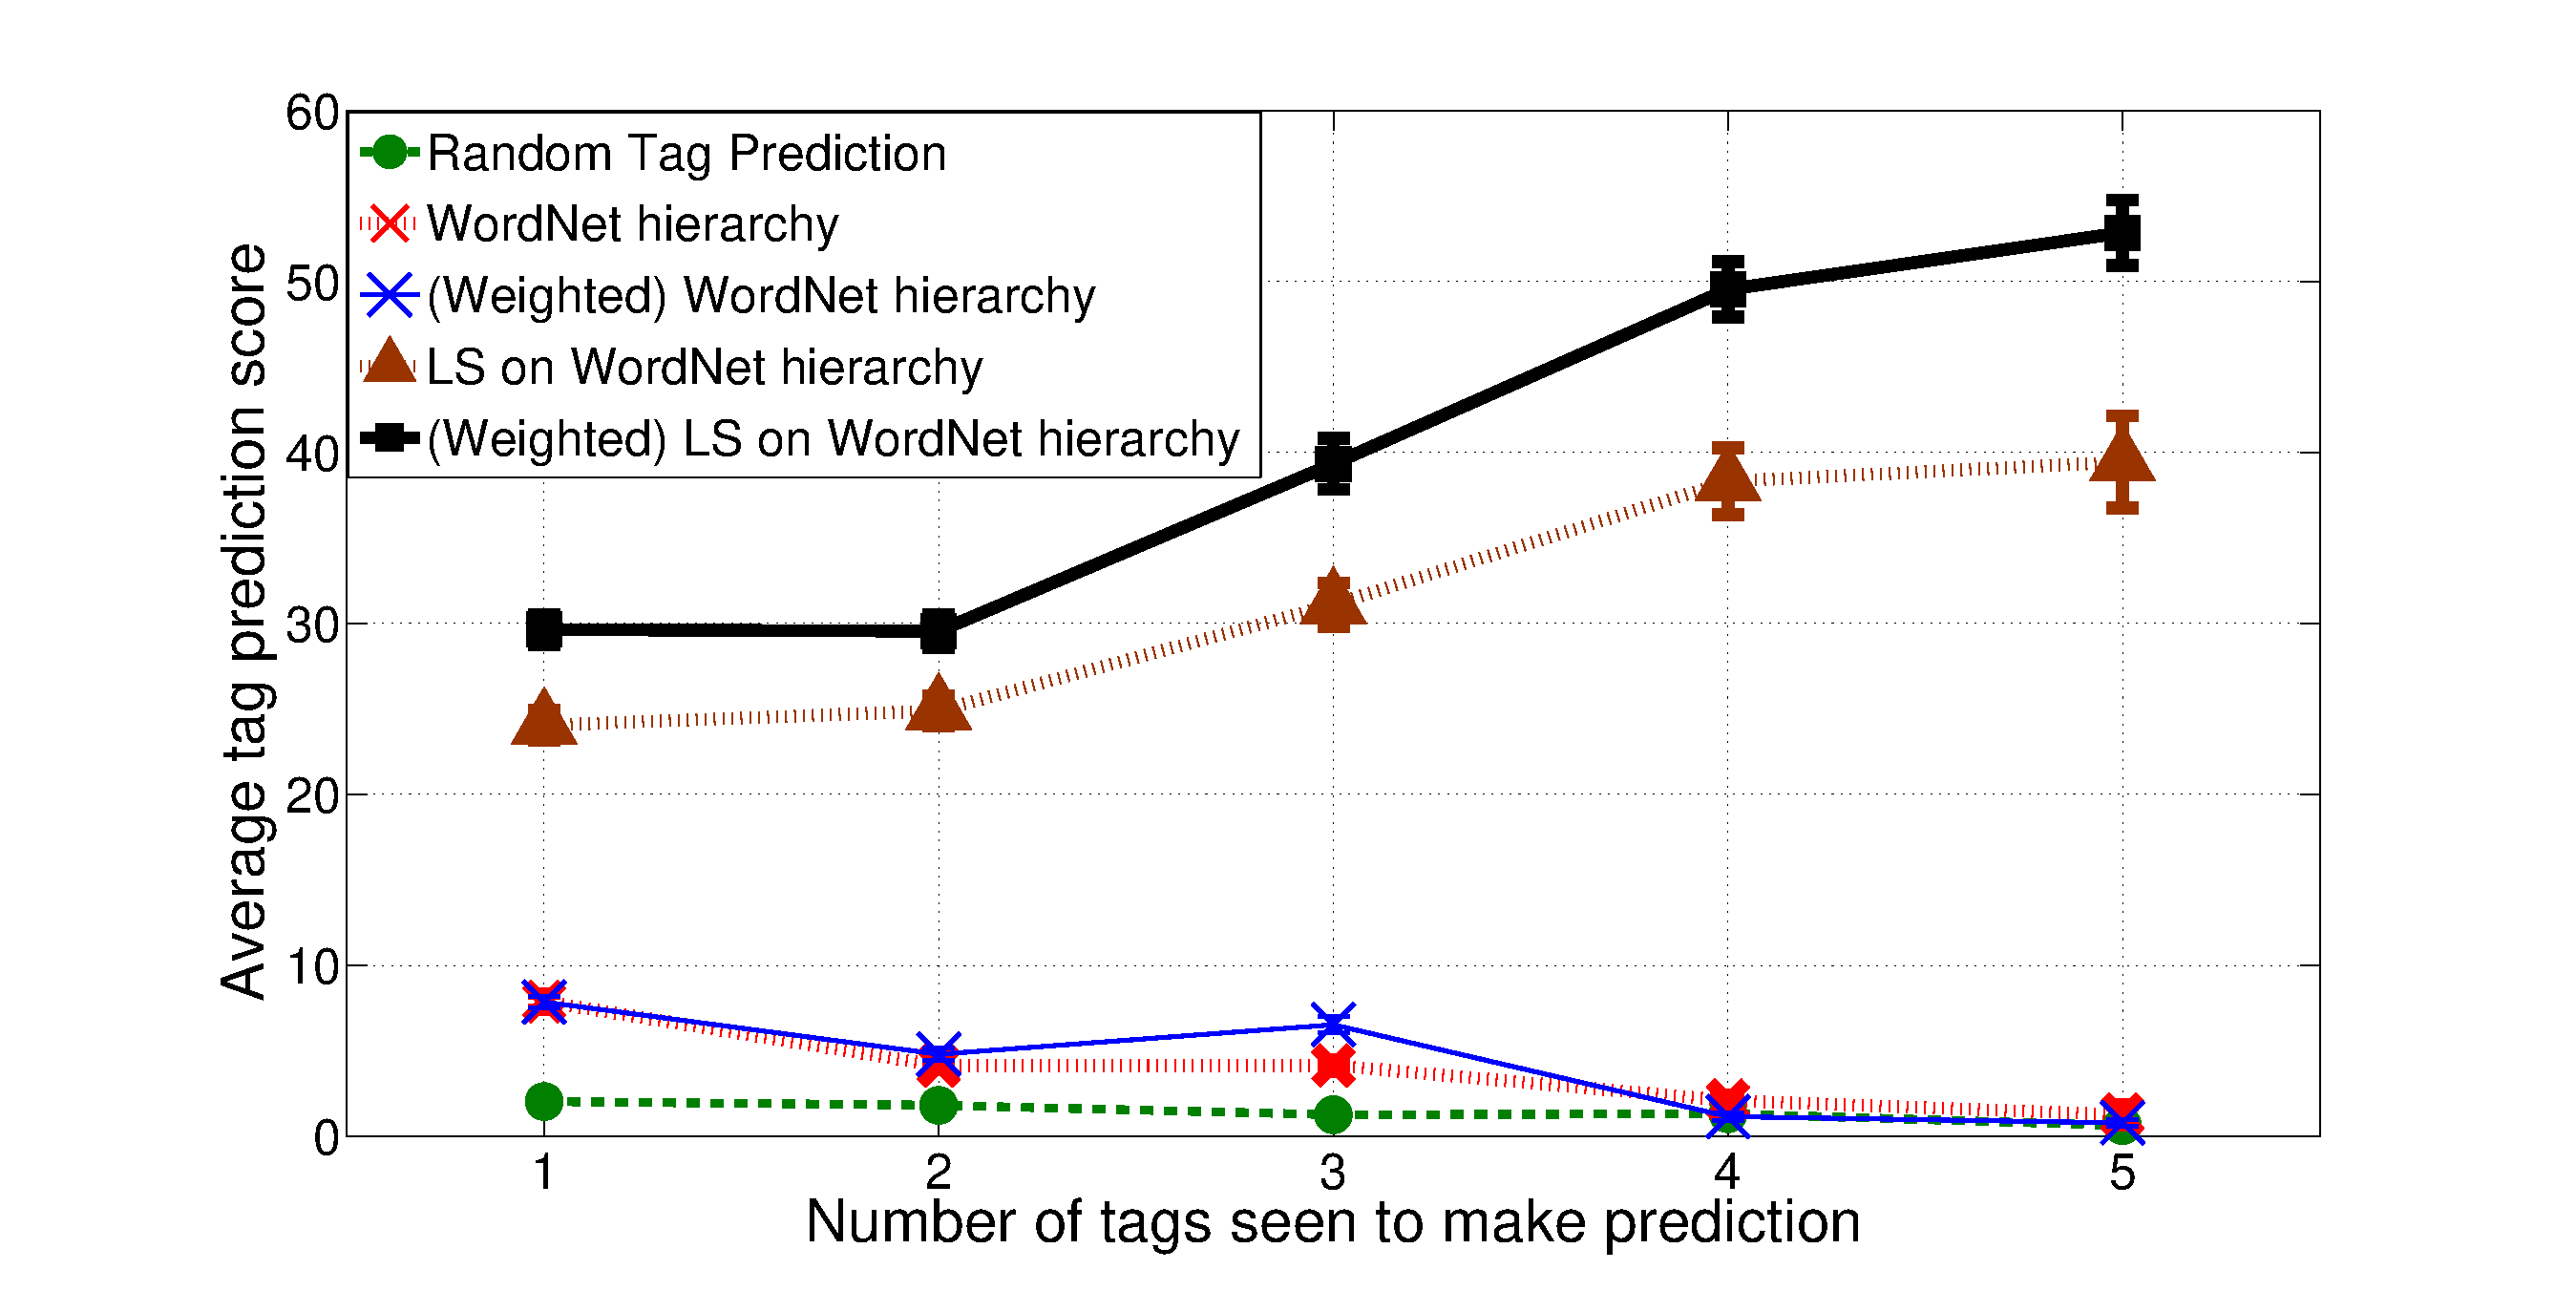
\includegraphics[width=\linewidth]{FWS117TagPredResultsusingSTForCol}
%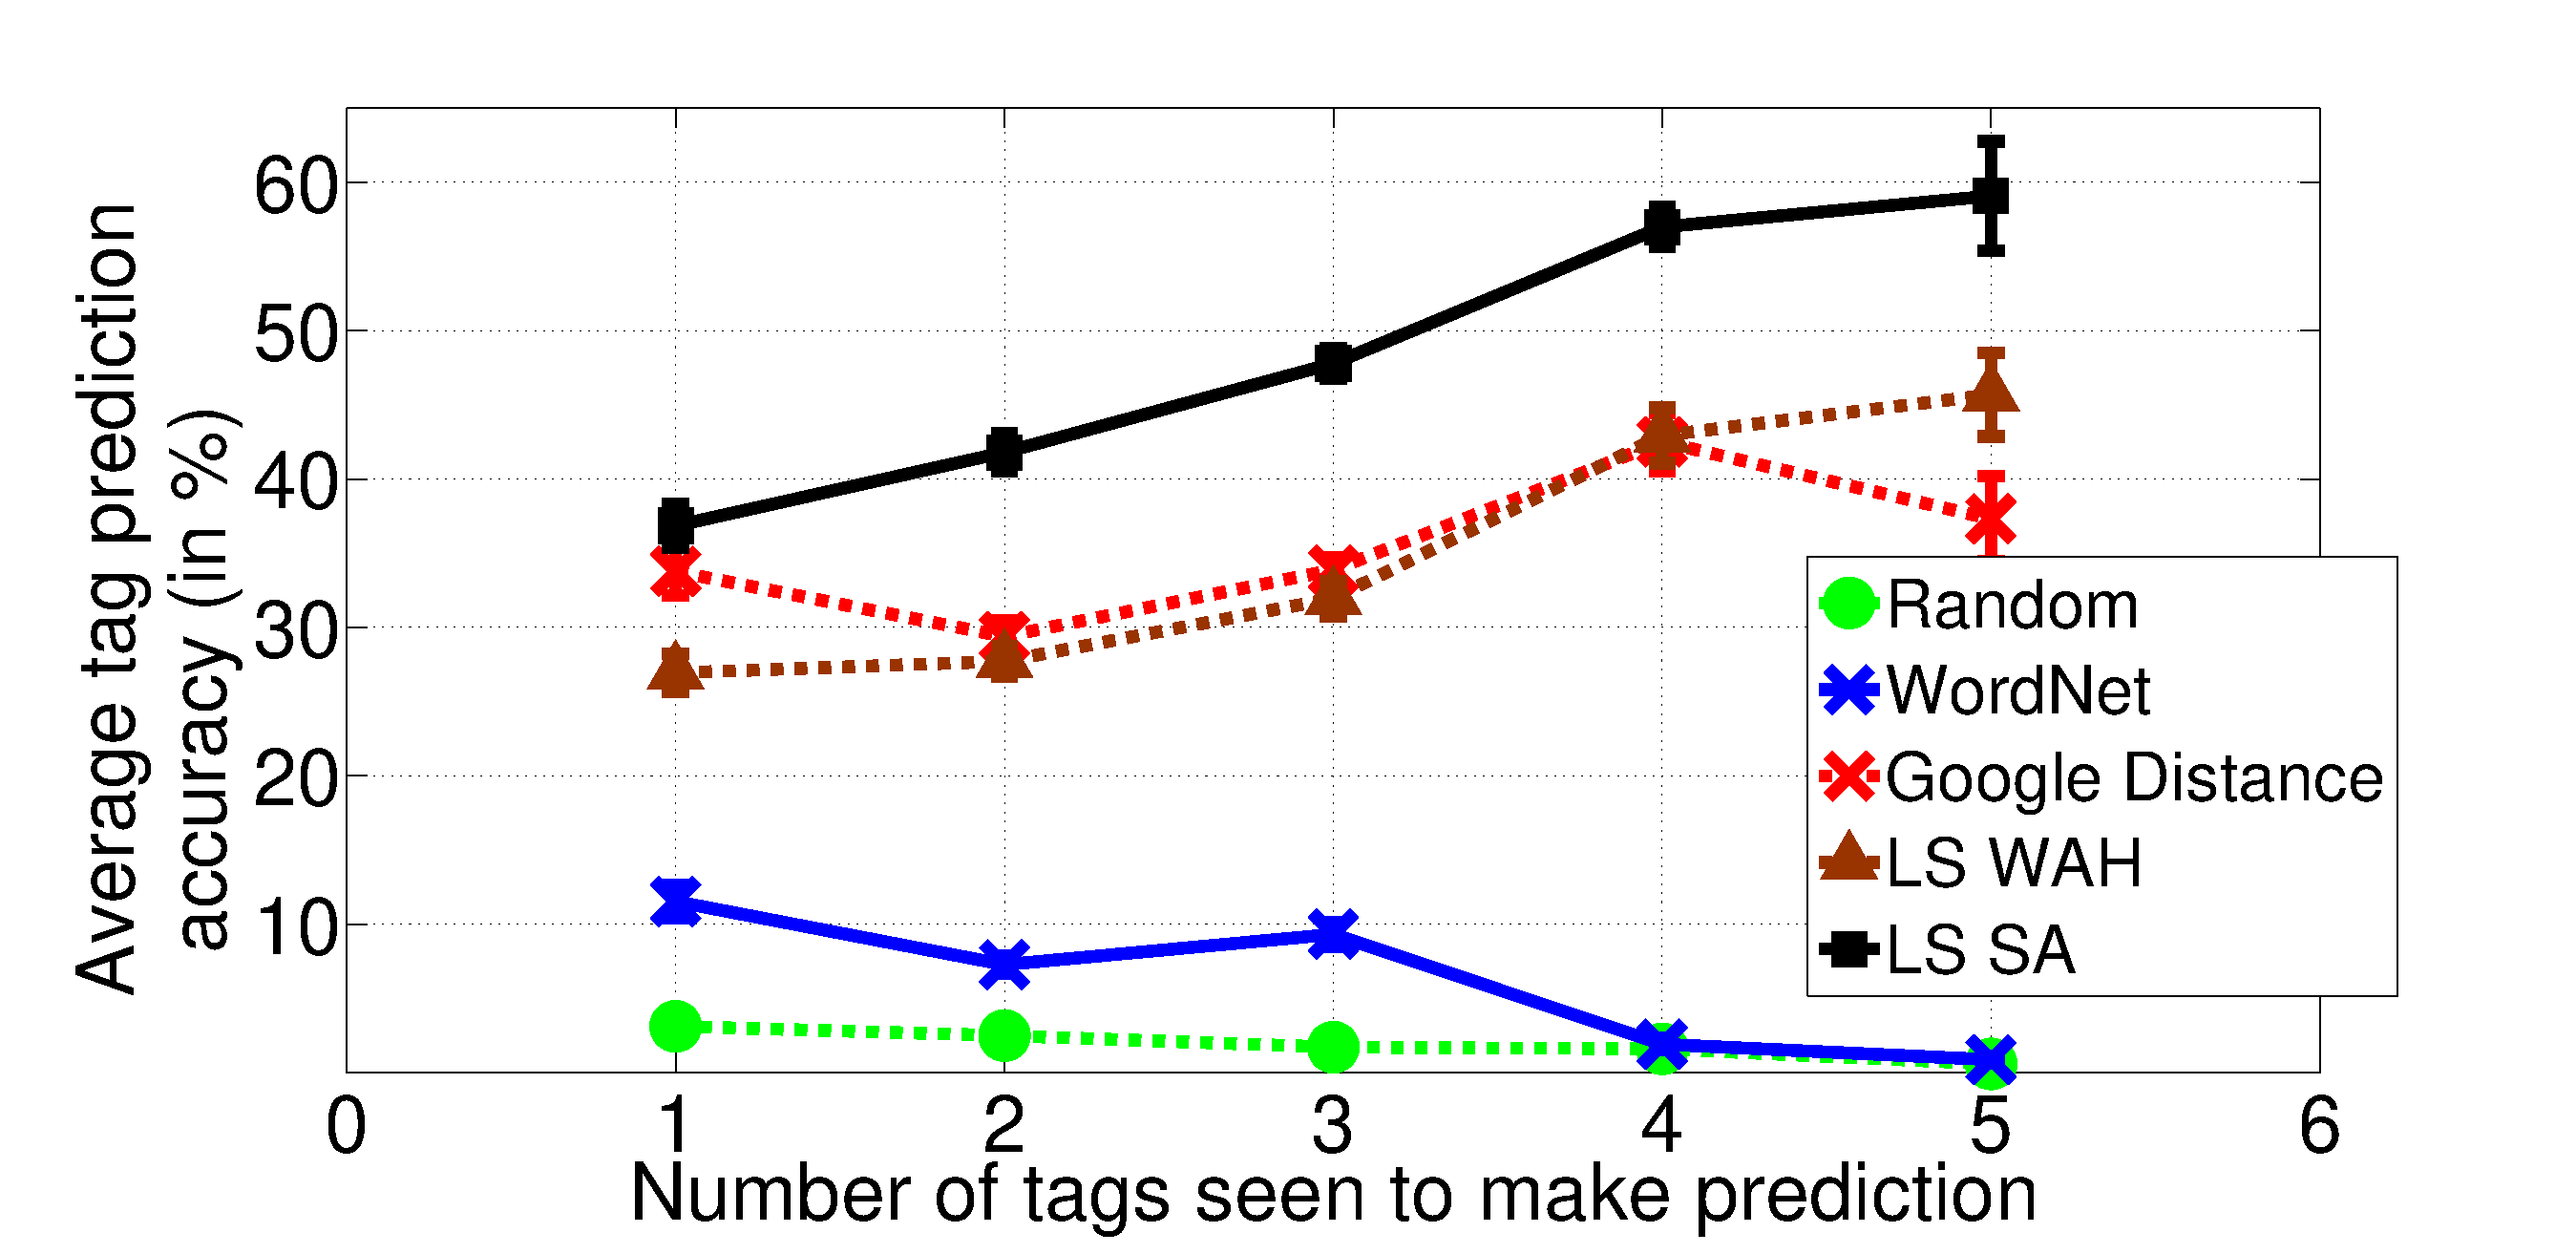
\includegraphics[width=\linewidth]{FlickrTPFig_journal}
\centering
\includegraphics[width=0.65\linewidth]{TagTree/TPFlickr_rebuttal}
\caption[Average Tag Prediction Accuracies marginalized over $N_{Tags}$ for various methods for the tag prediction task on Flickr corpus. ]{Average Tag Prediction Accuracies marginalized over $N_{Tags}$ for various methods for the tag prediction task on Flickr corpus. Note that Google Distance refers to the method corresponding to Google Similarity Distance as outlined in Section \ref{sec:comparison}.} 
\label{fig:FWS117TagPredGraph}
\end{figure}
\begin{table}
\fontsize{8pt}{1em}\selectfont
\begin{center}
\caption{Average Tag Prediction Accuracies (in \%) obtained using  Random method on Flickr corpus.}
%\vspace{-0.2in}
\label{tab:TPFlickr117Random}
\begin{tabular}{|p{2cm}|c|c|c|c|c|}
		\hline
		{$\boldsymbol{N_{Seen} \rightarrow}$} & &  &  &  &\\ 
		{$\boldsymbol{N_{Tags}} \downarrow $} & \textbf{1} & \textbf{2} & \textbf{3} & \textbf{4} & \textbf{5}   \\ 
		\hline 		
		\textbf{2} & 1.57 & - & - & - & -\\ 
		\hline
		\textbf{3} & 2.34 & 1.30 & - & - & -\\ 
		\hline
		\textbf{4} & 2.67 & 1.55 & 0.73 & - & -\\ 
		\hline
		\textbf{5} & 2.19 & 1.68 & 1.01 & 0.78 & -\\ 
		\hline
		\textbf{6} & 6.80 & 5.39 & 3.36 & 2.41 & 0.58 \\ 
		\hline
\end{tabular}
\vspace{-2mm}
\end{center}
\end{table}
\begin{table}
\fontsize{8pt}{1em}\selectfont
\begin{center}
\caption{Average Tag Prediction Accuracies (in \%) obtained using WordNet method on Flickr corpus.} 
\label{tab:TPFlickr117Wordnet}
\begin{tabular}{|p{2cm}|c|c|c|c|c|}
		\hline
		{$\boldsymbol{N_{Seen} \rightarrow}$} & &  &  &  &\\ 
		{$\boldsymbol{ N_{Tags}} \downarrow$} & \textbf{1} & \textbf{2} & \textbf{3} & \textbf{4} & \textbf{5}   \\ 	
		\hline
		\textbf{2} & 7.05 & - & - & - & -\\ 
		\hline
		\textbf{3} & 8.17 & 2.88 & - & - & -\\ 
		\hline
		\textbf{4} & 11.16 & 5.27 & 5.39 & - & -\\ 
		\hline
		\textbf{5} & 16.50 & 10.05 & 13.10 & 0.84 & -\\ 
		\hline
		\textbf{6} & 14.72 & 10.85 & 9.46 & 2.97 & 0.87 \\ 
		\hline
\end{tabular}
\vspace{-2mm}
\end{center}
\end{table}
\begin{table}
\fontsize{8pt}{1em}\selectfont
\begin{center}
\caption{Average Tag Prediction Accuracies (in \%) obtained using Google Similarity Distance method on Flickr corpus.} 
\label{tab:TPFlickr117Google}
\begin{tabular}{|p{2cm}|c|c|c|c|c|}
		\hline
		{$\boldsymbol{N_{Seen} \rightarrow}$} & &  &  &  &\\ 
		{$\boldsymbol{ N_{Tags}} \downarrow$} & \textbf{1} & \textbf{2} & \textbf{3} & \textbf{4} & \textbf{5}   \\ 	
		\hline
		\textbf{2} & 22.07 & - & - & - & -\\ 
		\hline
		\textbf{3} & 17.01 & 5.50 & - & - & -\\ 
		\hline
		\textbf{4} & 23.70 & 16.67 & 11.66 & - & -\\ 
		\hline
		\textbf{5} & 51.51 & 47.09 & 45.28 & 43.15 & -\\ 
		\hline
		\textbf{6} & 54.55 & 48.28 & 44.68 & 41.85 & 37.30 \\ 
		\hline
\end{tabular}
\vspace{-2mm}
\end{center}
\end{table}
\begin{table}[!htb]
\fontsize{8pt}{1em}\selectfont
\begin{center}
\caption{Average Tag Prediction Accuracies (in \%) obtained using LS-WAH method on Flickr corpus.} 
\label{tab:TPFlickr117LSWAH}
\begin{tabular}{|p{2cm}|c|c|c|c|c|}
		\hline
		{$\boldsymbol{N_{Seen} \rightarrow}$} & &  &  &  &\\ 
		{$\boldsymbol{ N_{Tags}} \downarrow$} & \textbf{1} & \textbf{2} & \textbf{3} & \textbf{4} & \textbf{5}   \\ 	
		\hline
		\textbf{2} & 16.13 & - & - & - & -\\ 
		\hline
		\textbf{3} & 11.53 & 5.51 & - & - & -\\ 
		\hline
		\textbf{4} & 14.91 & 10.96 & 7.17 & - & -\\ 
		\hline
		\textbf{5} & 42.76 & 42.94 & 39.69 & 36.95 & -\\ 
		\hline
		\textbf{6} & 49.37 & 51.48 & 49.00 & 48.89 & 45.69 \\ 
		\hline
\end{tabular}
\vspace{-2mm}
\end{center}
\end{table}
\begin{table}[!htb]
\fontsize{8pt}{1em}\selectfont
\begin{center}
\caption{Average Tag Prediction Accuracies (in \%) obtained using LS-SA method on Flickr corpus.}
\label{tab:TPFlickr117LSSA}
\begin{tabular}{|p{2cm}|c|c|c|c|c|}
		\hline
		%\textbf{$N_{Tags}$, $N_{Seen}$} & \textbf{1} & \textbf{2} & \textbf{3} & \textbf{4} & \textbf{5} \\ 
		{$\boldsymbol{N_{Seen} \rightarrow}$} & &  &  &  &\\ 
		{$\boldsymbol{N_{Tags}}\downarrow $} & \textbf{1} & \textbf{2} & \textbf{3} & \textbf{4} & \textbf{5}   \\ 
		\hline 		
		\textbf{2} & 25.87 & - & - & - & -\\ 
		\hline
		\textbf{3} & 20.34 & 21.65 & - & - & -\\ 
		\hline
		\textbf{4} & 26.09 & 28.96 & 26.43 & - & -\\ 
		\hline
		\textbf{5} & 52.33 & 54.79 & 54.82 & 53.16 & -\\ 
		\hline
		\textbf{6} & 59.57 & 61.78 & 62.10 & 60.81 & 59.07 \\ 
		\hline
\end{tabular}
\vspace{-2mm}
\end{center}
\end{table}
\begin{table}[!htb]
\fontsize{8pt}{1em}\selectfont
\begin{center}
\caption{\hl{Average Tag Prediction Accuracies (in \%) obtained using Symmetric sum method on Flickr corpus.}}
\label{tab:TPFlickr117Jij}
\begin{tabular}{|p{2cm}|c|c|c|c|c|}
		\hline
		%\textbf{$N_{Tags}$, $N_{Seen}$} & \textbf{1} & \textbf{2} & \textbf{3} & \textbf{4} & \textbf{5} \\ 
		{$\boldsymbol{N_{Seen} \rightarrow}$} & &  &  &  &\\ 
		{$\boldsymbol{N_{Tags}}\downarrow $} & \textbf{1} & \textbf{2} & \textbf{3} & \textbf{4} & \textbf{5}   \\ 
		\hline 		
		\textbf{2} &\hl{ 25.62} & - & - & - & -\\
		\hline
		\textbf{3} & \hl{21.19} & \hl{22.17} & - & - & - \\
		\hline
		\textbf{4} & \hl{28.69} & \hl{30.88} & \hl{28.12} & - & - \\
		\hline
		\textbf{5} & \hl{55.6} & \hl{57.88} & \hl{57.12} & \hl{54.27} & - \\
		\hline
		\textbf{6} & \hl{62.77} & \hl{65.48} & \hl{67.05} & \hl{66.35} & \hl{63.75} \\
		\hline
\end{tabular}
\vspace{-2mm}
\end{center}
\end{table}


%For completeness, we also provide the Average Tag Prediction Scores for various combinations of $N_{Tags}$ and $N_{Seen}$ in Tables~\ref{tab:TPFlickr117Random} - Table~\ref{tab:TPFlickr117GDWordNetSTJaccardWeight}. It is clear that the proposed approach greatly improves the performance compared to the WordNet based methods for all combinations of $N_{Tags}$ and $N_{Seen}$.
We provide examples of some test images from the Flickr corpus that had $N_{Tags}$=5 and $N_{Seen}$=2. Fig.~\ref{fig:positiveExs} shows a few test images for which LS-SA method made 100\% correct predictions. Fig. \ref{fig:negativeExs} shows test images that gave 0\% tag prediction accuracies. The corresponding sets of seen ($\mathcal{T}_{i,Seen}$), unseen ($\mathcal{T}_i \setminus  \mathcal{T}_{i,Seen}$), and the predicted tags ($\mathbb{P}_i$) are also provided. 


%Table~\ref{tab:TPFlickr117WordNetST}, the Average Tag Prediction Score for  $N_{Tags}=5$ and $N_{Seen}=3$ is only about 4.1\%. Compare this to the score obtained by proposed approach, as shown in Table~\ref{tab:TPFlickr117GDWordNetST}: 40.3\%! 





\textbf{Stock images corpus:} As in the Flickr corpus, we first select the set of most popular tags from the corpus of stock images that are also in WordNet. This produces a set $\mathcal{T}$, of 30 tags. Tables \ref{tab:TPGWS30Random} through \ref{tab:TPGWS30Jij} show the Average Tag Prediction Accuracies for various combinations of $N_{Tags}$ and $N_{Seen}$ for the tag prediction methods discussed in Section \ref{sec:comparison}. 
The Average Tag Prediction Accuracies marginalized over $N_{Tags}$ are shown in  Fig.~\ref{fig:GWS30TagPredGraph}, plotted as a function of $N_{Seen}$.  
%The total number of tags in an image, $N_{Tags}$ is varied from 2 to 10 such that $N_{Seen}$ varies from 1 to ($N_{Tags}-1$).  
Note that if $N_{Tags}$ is kept constant, increasing $N_{Seen}$ reduces the number of unseen tags (i.e., $\mathcal{T}_i \setminus  \mathcal{T}_{i,Seen}$), thus reducing the random chance of predicting a correct unseen tag from $\mathcal{T} \setminus \mathcal{T}_{i,Seen}$.  As a result of this phenomenon, a drop in performance for random prediction and other methods can be seen with increasing $N_{Seen}$. \\
\begin{figure}[!ht]
%\epsfig{width=10cm,figure=GWS20TagPredColumnMeanResultsForST.eps}
%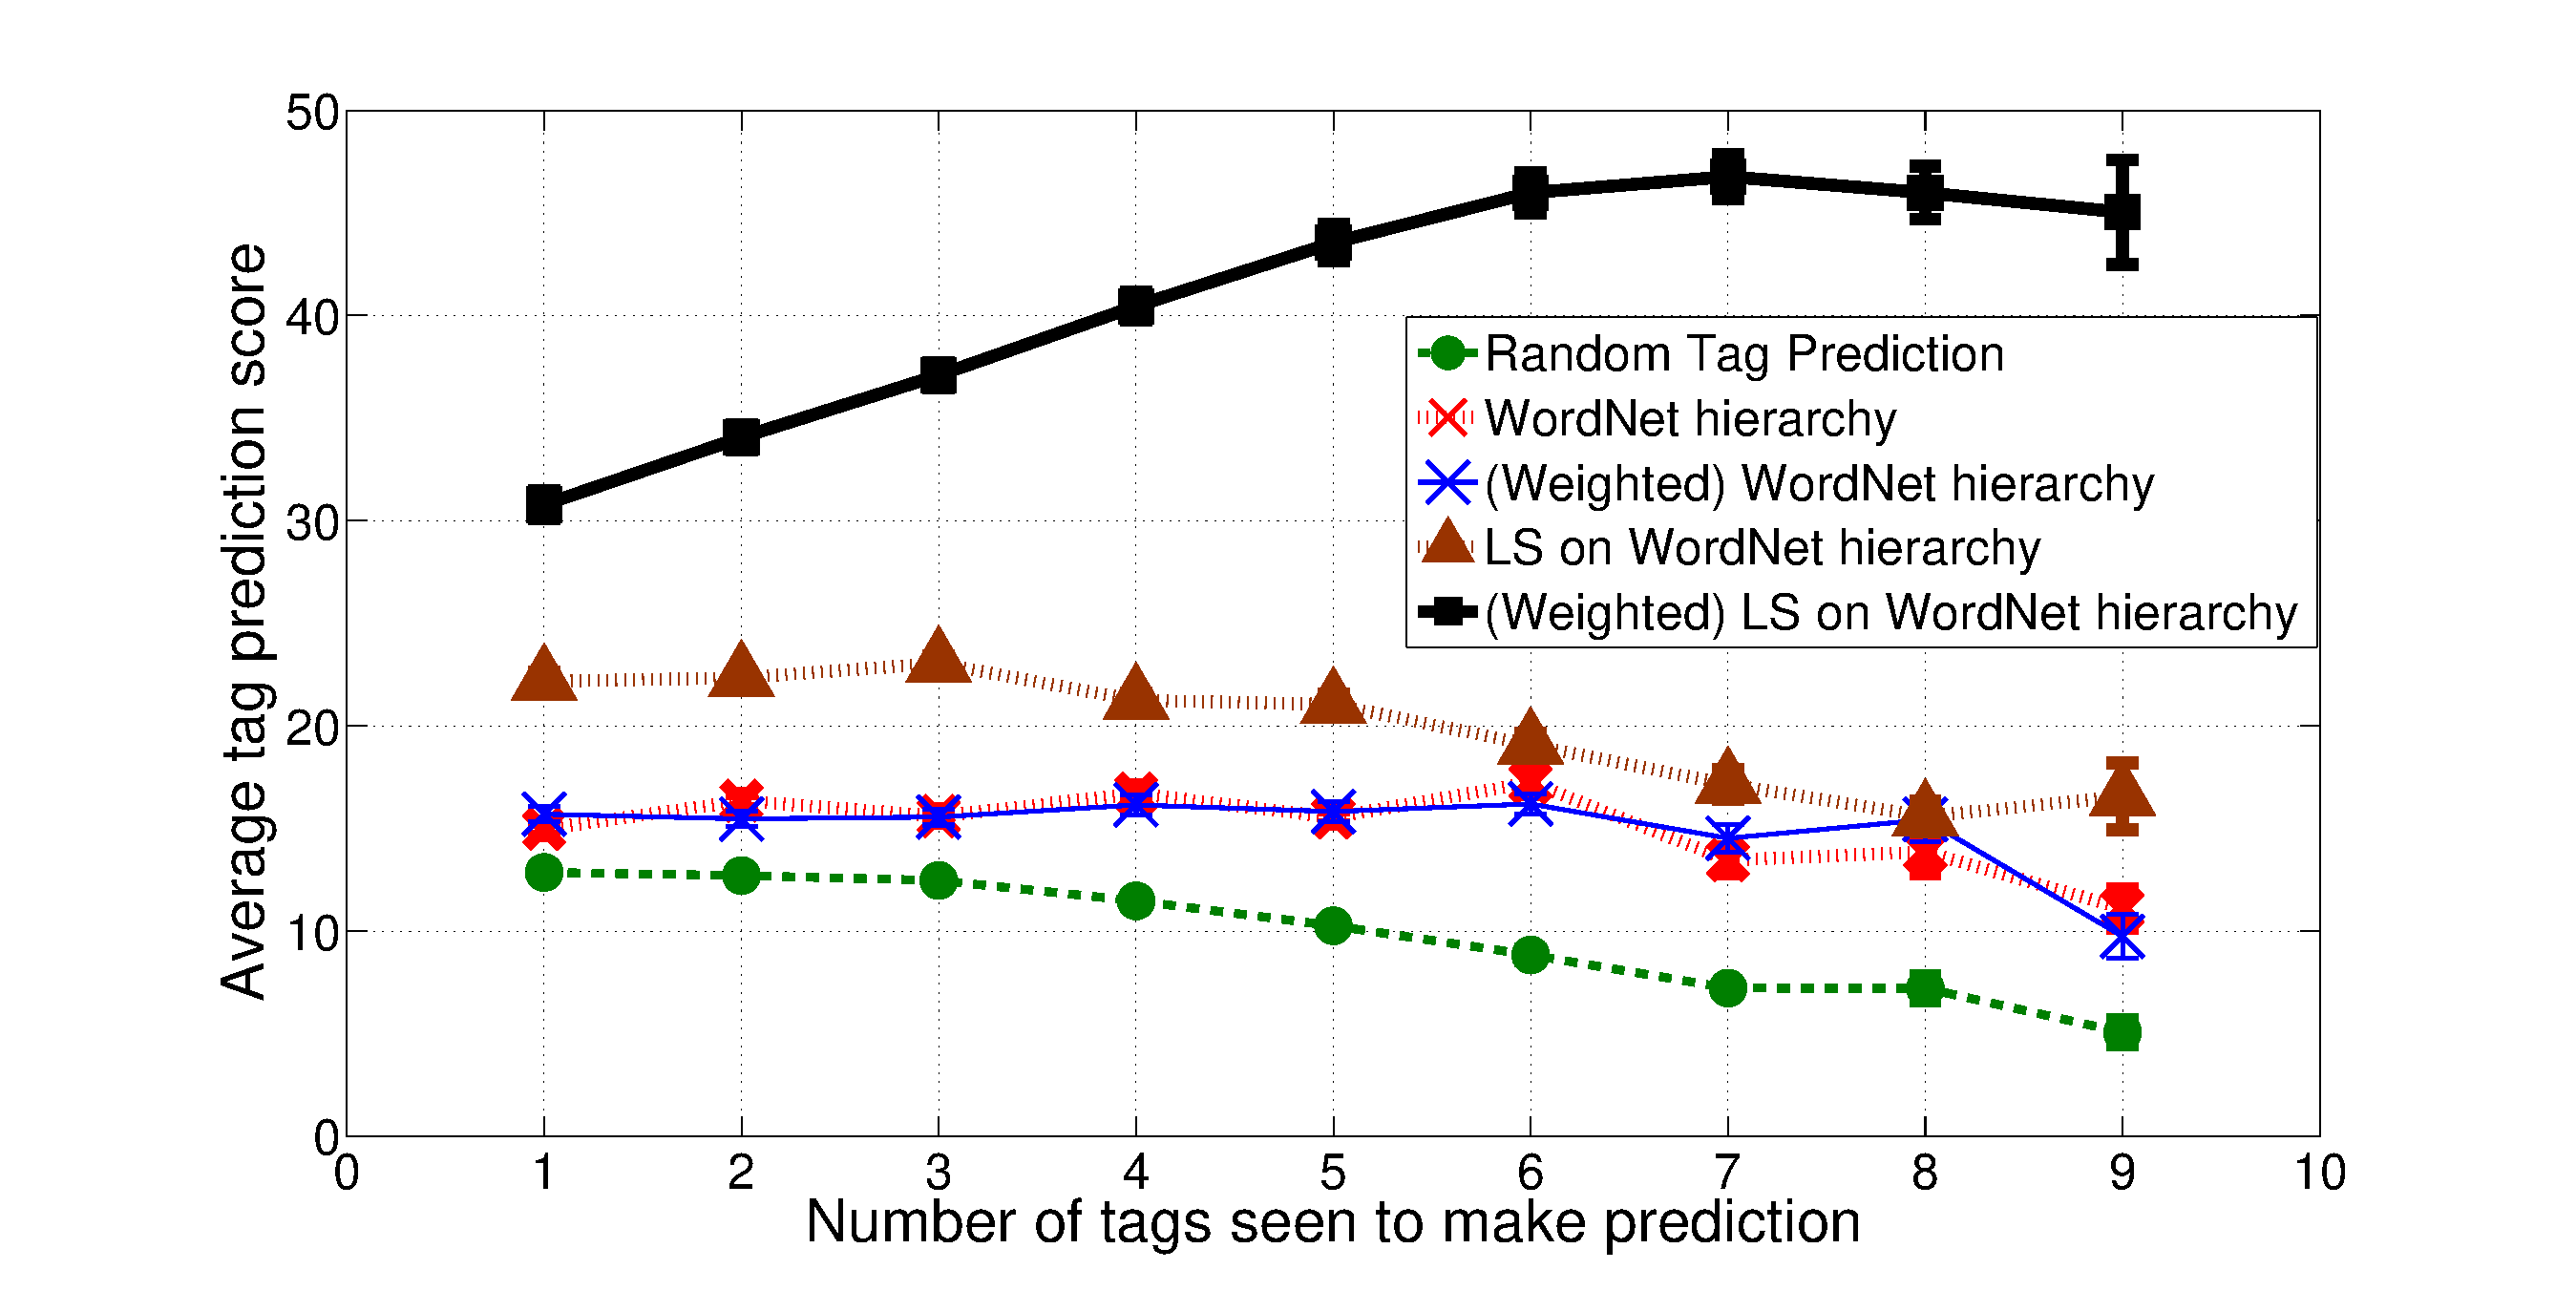
\includegraphics[width=\linewidth]{GWS20TagPredColumnMeanResultsForST}
%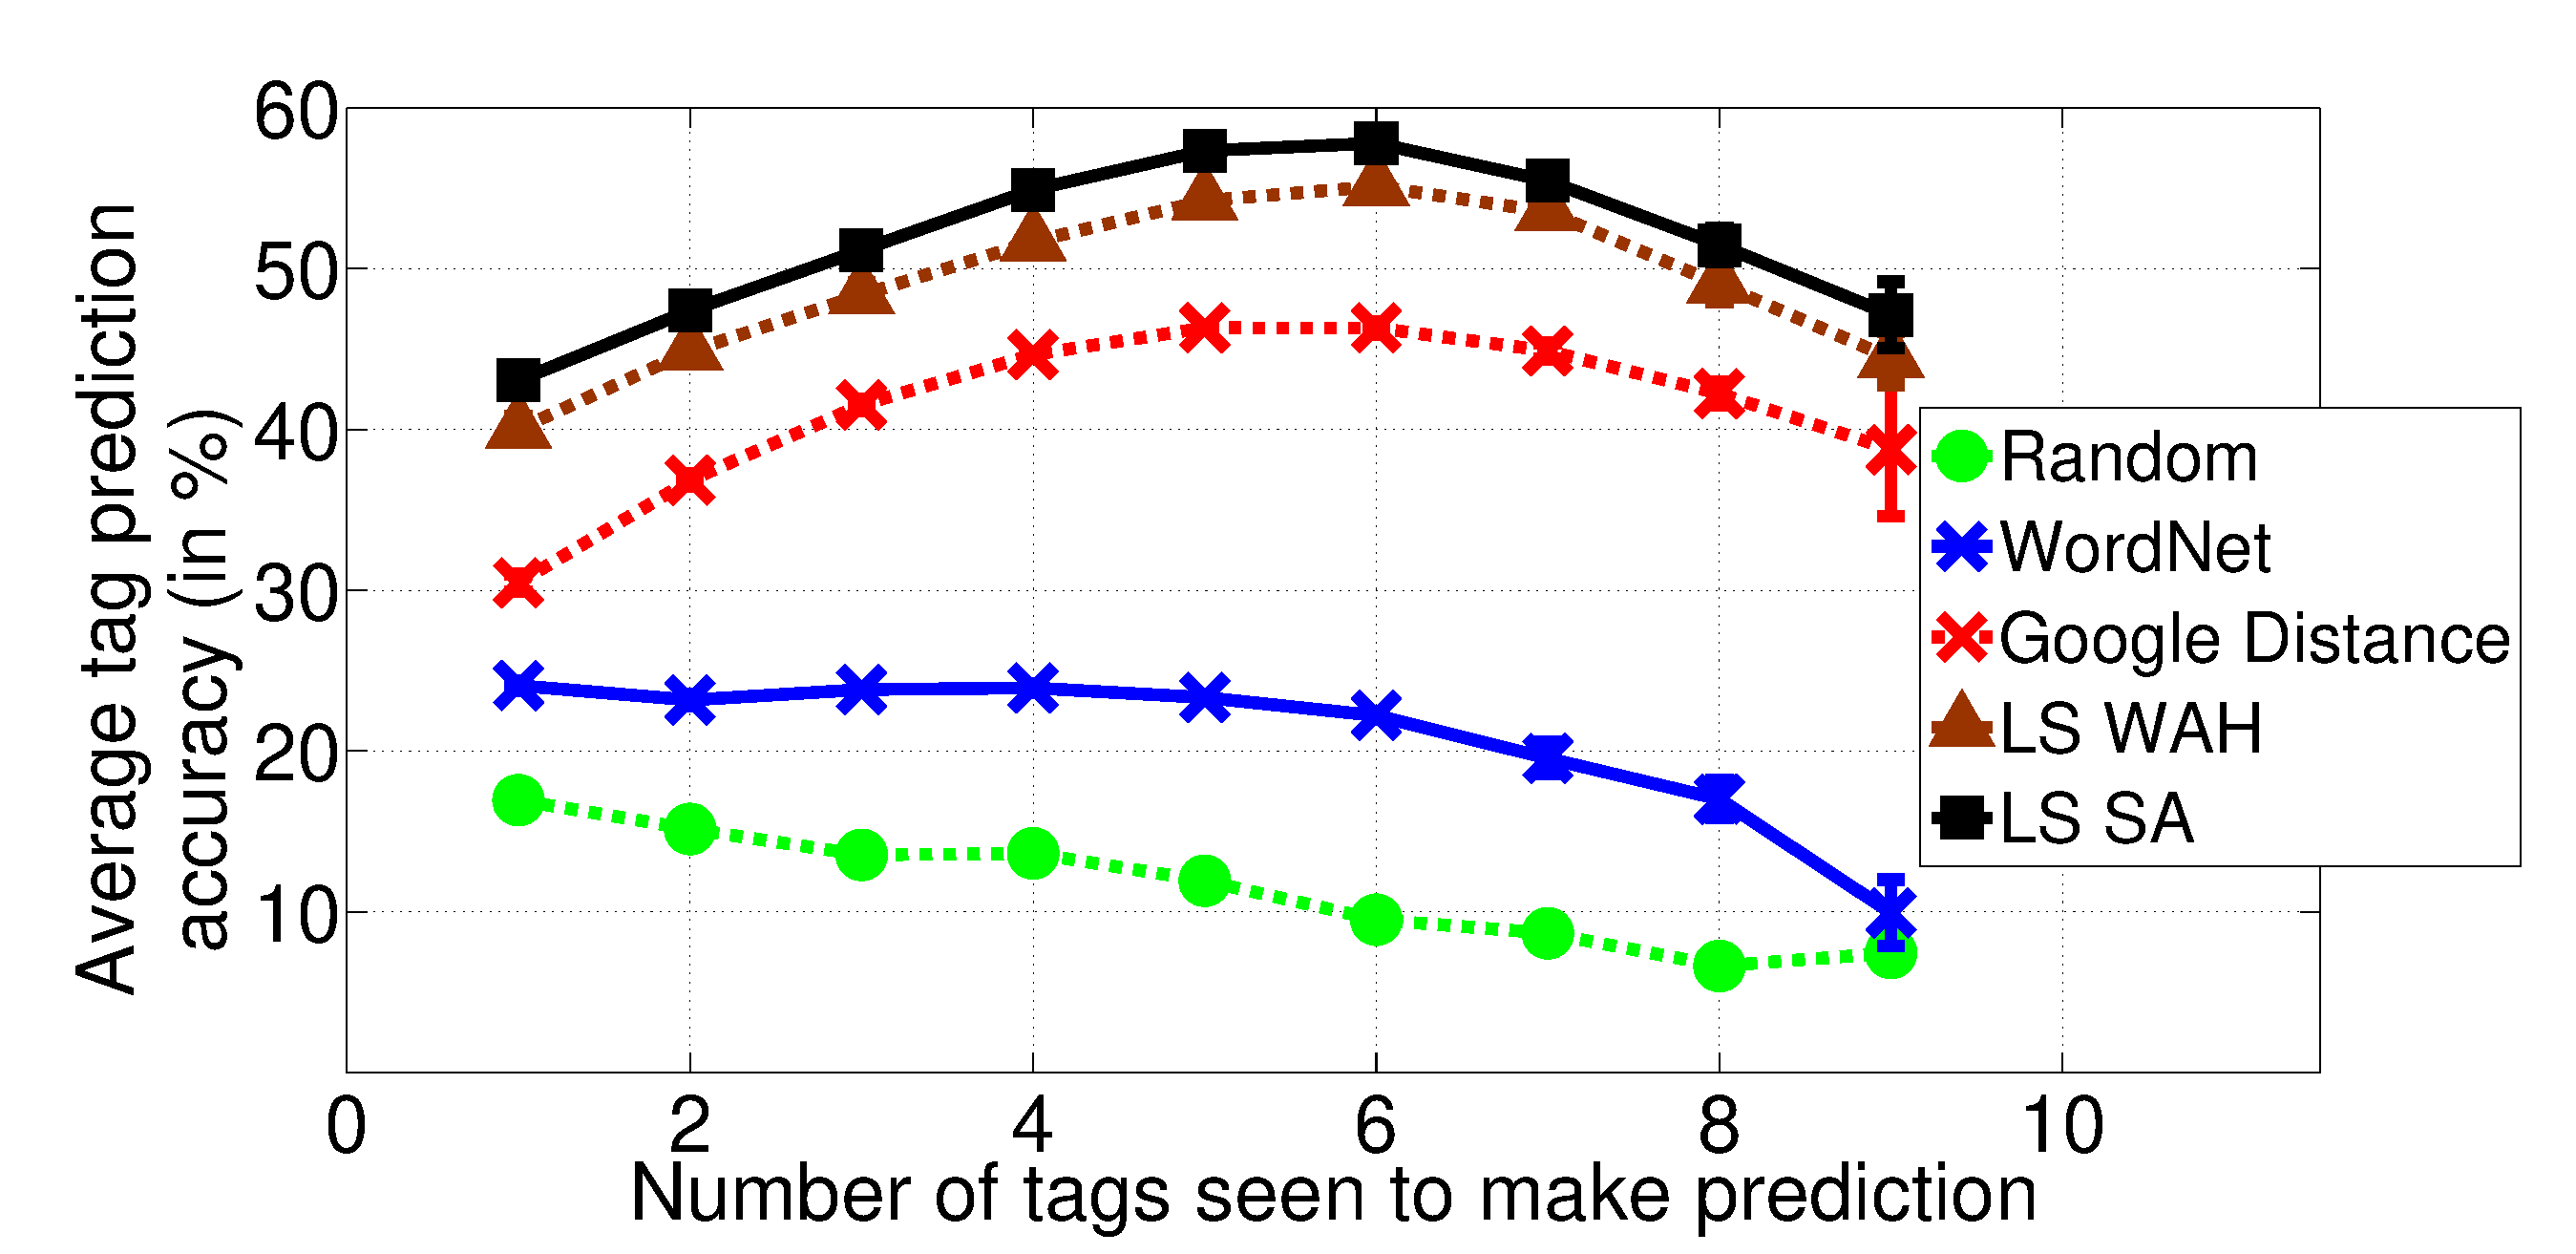
\includegraphics[width=\linewidth]{GWS30_tagPredFig_Journal}
\centering
\includegraphics[width=0.65\linewidth]{TagTree/RebuttalGWS_TP}
\caption{\hl{Average Tag Prediction Accuracies marginalized over $N_{Tags}$ for various methods for the tag prediction task on Stock images corpus.}}
\label{fig:GWS30TagPredGraph}
\end{figure}
\begin{table}[!htbp]
\fontsize{8pt}{1em}\selectfont
\begin{center}
\caption{Average Tag Prediction Accuracies (in \%) obtained using Random method on Stock images corpus.}
\label{tab:TPGWS30Random}
\begin{tabular}{|p{1.5cm}|p{0.5cm}|p{0.5cm}|p{0.5cm}|p{0.5cm}|p{0.5cm}|p{0.5cm}|p{0.5cm}|p{0.5cm}|p{0.5cm}|}
		\hline
		{$\boldsymbol{N_{Seen} \rightarrow}$} & &  &  &  & &  &  &  &\\ 
		{$\boldsymbol{N_{Tags}} \downarrow $} & \textbf{1} & \textbf{2} & \textbf{3} & \textbf{4} & \textbf{5}  & \textbf{6} & \textbf{7} & \textbf{8} & \textbf{9} \\ 
		\hline 		
		\textbf{2} & 1&-&-&-&-&-&-&-&- \\
		\hline
		\textbf{3} & 7&5.28&-&-&-&-&-&-&- \\
		\hline
		\textbf{4} & 11.3&5.8&4.9&-&-&-&-&-&-\\
		\hline
		\textbf{5} & 14.9&10.1&6.8&6.1&-&-&-&-&- \\
		\hline
		\textbf{6} & 19.1&12.9&10.1&9.5&3.1&-&-&-&- \\
		\hline
		\textbf{7} & 21.5&16.1&14.6&10.1&13.1&2.5&-&-&- \\ 
		\hline
		\textbf{8} & 20.7&17.8&11.8&12.7&6.4&9.6&2.3&-&- \\
		\hline
		\textbf{9} & 28.6&25.5&23&19.8&19.4&12.4&7&5.7&- \\ 
		\hline
		\textbf{10} & 28.3&27.6&23.5&23.5&17.7&13.6&16.7&7.6&7.4 \\ 
		\hline
\end{tabular}
\vspace{-2.5mm}
\end{center}
\end{table}
%It is clear that the tag trees built using the proposed approach outperform the baseline graphs constructed using WordNet for all values of $N_{Seen}$. 
%The detailed tables containing Average Tag Prediction Scores for all values of $N_{Tags}$ and $N_{Seen}$ are omitted for brevity but the trend is similar to the one observed for the Flickr corpus.
%\vspace{-5mm}
% The tag prediction score is higher when edge weights of constructed semantic graph are taken as Jaccard similarities between connecting tags. Readers should note however that the improvement is not entirely because of edge weights being Jaccard similarities. Rather, the edges in semantic graph obtain by proposed approach captures corpus specific information in a much more effective manner than semantics-based graphs such as obtained from WordNet. This can be verified by the consistent gap in performance for edge weights being 1, and Jaccard similarities. 
\begin{table}[!htbp]
\fontsize{8pt}{1em}\selectfont
\begin{center}
\caption{Average Tag Prediction Accuracies (in \%) obtained using WordNet method on Stock images corpus.}
\label{tab:TPGWS30Wordnet}
\begin{tabular}{|p{1.5cm}|p{0.5cm}|p{0.5cm}|p{0.5cm}|p{0.5cm}|p{0.5cm}|p{0.5cm}|p{0.5cm}|p{0.5cm}|p{0.5cm}|}
		\hline
		{$\boldsymbol{N_{Seen} \rightarrow}$} & &  &  &  & &  &  &  &\\ 
		{$\boldsymbol{N_{Tags}}\downarrow $} & \textbf{1} & \textbf{2} & \textbf{3} & \textbf{4} & \textbf{5}  & \textbf{6} & \textbf{7} & \textbf{8} & \textbf{9} \\ 
		\hline 		
		\textbf{2} & 1.9&-&-&-&-&-&-&-&- \\
		\hline
		\textbf{3} & 8.9&3.3&-&-&-&-&-&-&- \\
		\hline
		\textbf{4} & 14.2&10.9&3.4&-&-&-&-&-&- \\
		\hline
		\textbf{5} & 21.3&16.9&14.7&8.5&-&-&-&-&- \\
		\hline
		\textbf{6} & 28.4&22.8&22&16.7&9.8&-&-&-&- \\
		\hline
		\textbf{7} & 32.3&28.4&28.4&24.8&22.4&12.6&-&-&- \\
		\hline
		\textbf{8} & 35.7&33.3&32.7&30.7&27.6&23.8&13&-&- \\
		\hline
		\textbf{9} & 36.5&34.5&32.7&31.9&28.7&26.3&23.4&15.5&- \\
		\hline
		\textbf{10} & 37.4&35.2&32.9&30.8&28&26.1&22.3&18.5&9.9 \\
		\hline
\end{tabular}
\vspace{-2.5mm}
\end{center}
\end{table}
\begin{table}[~htp]
\fontsize{8pt}{1em}\selectfont
\begin{center}
\caption{Average Tag Prediction Accuracies (in \%) obtained using Google Similarity Distance method on Stock images corpus.}
\label{tab:TPGWS30Google}
\begin{tabular}{|p{1.5cm}|p{0.5cm}|p{0.5cm}|p{0.5cm}|p{0.5cm}|p{0.5cm}|p{0.5cm}|p{0.5cm}|p{0.5cm}|p{0.5cm}|}
		\hline
		{$\boldsymbol{N_{Seen} \rightarrow}$} & &  &  &  & &  &  &  &\\ 
		{$\boldsymbol{N_{Tags}}\downarrow $} & \textbf{1} & \textbf{2} & \textbf{3} & \textbf{4} & \textbf{5}  & \textbf{6} & \textbf{7} & \textbf{8} & \textbf{9} \\ 
		\hline 		
		\textbf{2} & 3.5&-&-&-&-&-&-&-&- \\
		\hline
		\textbf{3} & 11.2&8.4&-&-&-&-&-&-&- \\
		\hline
		\textbf{4} & 24&26.6&21.9&-&-&-&-&-&- \\
		\hline
		\textbf{5} & 32.3&39.8&39.7&35.2&-&-&-&-&- \\
		\hline
		\textbf{6} & 36.6&43.9&46.5&46.5&44.5&-&-&-&- \\
		\hline
		\textbf{7} & 39.4&44.8&47.8&49.5&49.5&48.5&-&-&- \\
		\hline
		\textbf{8} & 43.6&45.2&47.3&48.5&49.1&49&48.7&-&- \\
		\hline
		\textbf{9} & 41.9&43.5&44.4&45.4&45.9&45.8&45.2&44.9&- \\
		\hline
		\textbf{10} & 41.6&42.7&43.2&42.8&42.6&42&40.7&39.5&38.7 \\
		\hline
\end{tabular}
\vspace{-2.5mm}
\end{center}
\end{table}
\begin{table}[!htp]
\fontsize{8pt}{1em}\selectfont
\begin{center}
\caption{Average Tag Prediction Accuracies (in \%) obtained using LS-WAH method on Stock images corpus.}
\label{tab:TPGWS30LSWAH}
\begin{tabular}{|p{1.5cm}|p{0.5cm}|p{0.5cm}|p{0.5cm}|p{0.5cm}|p{0.5cm}|p{0.5cm}|p{0.5cm}|p{0.5cm}|p{0.5cm}|}
		\hline
		{$\boldsymbol{N_{Seen} \rightarrow}$} & &  &  &  & &  &  &  &\\ 
		{$\boldsymbol{N_{Tags}}\downarrow $} & \textbf{1} & \textbf{2} & \textbf{3} & \textbf{4} & \textbf{5}  & \textbf{6} & \textbf{7} & \textbf{8} & \textbf{9} \\ 
		\hline 		
		\textbf{2} & 7.8&-&-&-&-&-&-&-&- \\
		\hline
		\textbf{3} & 14.6&15.4&-&-&-&-&-&-&- \\
		\hline
		\textbf{4} & 20.5&22.6&22&-&-&-&-&-&- \\
		\hline
		\textbf{5} & 36.2&33.2&32.8&31.3&-&-&-&-&- \\
		\hline
		\textbf{6} & 49&47.6&45.2&43.3&41.5&-&-&-&- \\
		\hline
		\textbf{7} & 59.6&59.4&58.7&57.1&54.4&51.4&-&-&- \\
		\hline
		\textbf{8} & 62.3&63.5&63.2&62.8&61.4&58.2&54.9&-&- \\
		\hline
		\textbf{9} & 56.6&59.7&59.2&58.7&57.9&56.3&52.8&49.5&- \\
		\hline
		\textbf{10} & 53.5&57.6&57.4&56.8&56.1&54.7&52.9&48.5&44.4 \\
		\hline
\end{tabular}
\vspace{-2.5mm}
\end{center}
\end{table}
\begin{table}[!htp]
\fontsize{8pt}{1em}\selectfont
\begin{center}
\caption{Average Tag Prediction Accuracies (in \%) obtained using LS-SA method on Stock images corpus.}
\label{tab:TPGWS30LSSA}
\begin{tabular}{|p{1.5cm}|p{0.5cm}|p{0.5cm}|p{0.5cm}|p{0.5cm}|p{0.5cm}|p{0.5cm}|p{0.5cm}|p{0.5cm}|p{0.5cm}|}
		\hline
		{$\boldsymbol{N_{Seen} \rightarrow}$} & &  &  &  & &  &  &  &\\ 
		{$\boldsymbol{N_{Tags}}\downarrow $} & \textbf{1} & \textbf{2} & \textbf{3} & \textbf{4} & \textbf{5}  & \textbf{6} & \textbf{7} & \textbf{8} & \textbf{9} \\ 
		\hline 		
		\textbf{2} & 7.2&-&-&-&-&-&-&-&- \\
		\hline
		\textbf{3} & 13.4&11.1&-&-&-&-&-&-&- \\ 
		\hline
		\textbf{4} & 28.4&27&21.1&-&-&-&-&-&- \\
		\hline
		\textbf{5} & 44.5&41.9&38.5&35&-&-&-&-&- \\
		\hline
		\textbf{6} & 53.3&53.3&51.3&49.5&46.9&-&-&-&- \\
		\hline
		\textbf{7} & 61.7&63.2&62.6&60.8&58.3&56&-&-&- \\
		\hline
		\textbf{8} & 64.3&64.8&65.8&65.3&63.1&60.2&57.4&-&- \\
		\hline
		\textbf{9} & 59&60.2&60.8&61.1&60.8&58&55.3&52.3&- \\
		\hline
		\textbf{10} & 55.7&57.7&57.9&57.8&57.6&57&53.7&50.6&47.1 \\
		\hline
\end{tabular}
\vspace{-2.5mm}
\end{center}
\end{table}

\begin{table}[!htp]
\fontsize{8pt}{1em}\selectfont
\begin{center}
\caption{\hl{Average Tag Prediction Accuracies (in \%) obtained using the Symmetric sum approach on Stock images corpus.}}
\label{tab:TPGWS30Jij}
\begin{tabular}{|p{1.5cm}|p{0.5cm}|p{0.5cm}|p{0.5cm}|p{0.5cm}|p{0.5cm}|p{0.5cm}|p{0.5cm}|p{0.5cm}|p{0.5cm}|}
		\hline
		{$\boldsymbol{N_{Seen} \rightarrow}$} & &  &  &  & &  &  &  &\\ 
		{$\boldsymbol{N_{Tags}}\downarrow $} & \textbf{1} & \textbf{2} & \textbf{3} & \textbf{4} & \textbf{5}  & \textbf{6} & \textbf{7} & \textbf{8} & \textbf{9} \\ 
		\hline 		
		\textbf{2} & \hl{11.1} & -  & -  & -  & -  & -  & -  & -  & - \\
		\hline
		\textbf{3} & 16.9 & 17.7 & -  & -  & -  & -  & -  & -  & -\\ 
		\hline
		\textbf{4} & 32.1 & 32.5 & 29.7 & -  & -  & -  & -  & -  & - \\
		\hline
		\textbf{5} & 45.1 & 47.8 & 46.4 & 43.1 & -  & -  & -  & -  & - \\
		\hline
		\textbf{6} & 52.7 & 56 & 56.3 & 55.5 & 53.2 & -  & -  & -  & - \\
		\hline
		\textbf{7} & 62.1 & 64.6 & 64.9 & 63.9 & 62 & 59.9 & -  & -  & - \\
		\hline
		\textbf{8} & 64.5 & 68 & 68.1 & 67.8 & 65.8 & 63.1 & 60.5 & -  & - \\
		\hline
		\textbf{9} & 60.6 & 63.9 & 64.9 & 64.9 & 64 & 61.5 & 58.5 & 55.9 & - \\
		\hline
		\textbf{10} & 58 & 61.5 & 62.9 & 63.2 & 63.1 & 61.6 & 58.9 & 55 & \hl{52.3}\\
		\hline
\end{tabular}
\vspace{-2.5mm}
\end{center}
\end{table}


\indent The results indicates that the proposed local search paradigm based approach has successfully adapted the ontological tag tree obtained from WordNet to the Flickr or stock images corpus. \hl{We can obtain performance better than or close to that of other tag prediction approaches, while having several orders of savings in the space requirement. } We next describe the second data-driven task used for evaluation of tag trees. 
\subsection{Efficient Classification Task}
\label{sec:effClassification}
\hl{We consider the problem of efficiently associating tags with resources based on the resource content. For domains where it is feasible to extract features from the resource and to train concept detectors, we show how tag trees can be utilized to determine which concept detectors should be applied on a given test resource. We demonstrate this using annotated image corpora and utilize different modalities to represent the content of a given resource. }
Given a test image, $i$ from the corpus without any associated tags or keywords, we predict which of the $N$ tags are applicable to the image. By letting each of the $N$ tags correspond to a category or class, this is equivalent to a multi-class, multi-label classification task. Let us assume that one-vs-all binary classifiers are available for each tag class - these take the image instance $i$ as input and can predict $P(j \mid i)$ where class $j$ corresponds to tag $t_j$. We can use this to predict whether or not a tag $t_j$ should be associated with image $i$ based on whether $P(j \mid i)$ is greater than an appropriate threshold $\theta$ or not. 

The naive approach to predict all tags applicable to $i$ would be to test each of the $N$ classifiers on $i$ and accumulate those tags for which the predictions by the corresponding classifiers exceed $\theta$. \hl{Some works such as {\cite{li2013classifying}} propose techniques to make classification of images faster. However in order to do this, these works require re-training of classifiers and cannot utilize existing classifiers for each tag. 
%For example {\cite{li2013classifying}} proposes an approach to select positive and negative examples determined most relevant with respect to a given concept. 
Contrary to these, in the proposed approach, we can utilize pre-trained classifiers corresponding to different tags. Other works such as the image annotation application in {\cite{wu2008flickr}} associate a test image with tags based on applying all concept detectors on the test image and then combining the predictions. However such approaches require applying all $N$ classifiers to a given test image and are hence inefficient for a large number of tags. }
This process can be made more efficient by using the ontological tag tree on the set of tags. Once certain labels have been predicted for an image $i$, one can utilize the tree structure to decide which tags are more or less likely to be associated with the image. Thus the choice of the classifiers to test next on the image $i$, can be made in a more efficient manner.  Therefore, a tag tree that captures the relations between the tags more effectively, is expected to lead to more efficient performance by reaching the correct number of predicted tags with fewer number of binary classifications performed. The \emph{efficient classification task} is formulated to measure the classification efficiency in such a setting. 

\indent This evaluation task is formulated as follows. Given $N$ binary classifiers, the $j^{th}$ classifier predicts probability $P(j \mid i)$ of tag $t_j$ being associated with a test image $i$. $K$ binary classifications are performed for image $i$ and the set of tags that are predicted positive among those $K$ classifications, comprise the set of predicted tags $\mathbb{P}_{i,K}$ for image $i$ for given $K$. The ground truth set of tags that are associated with image $i$ as per the corpus, is denoted $\mathcal{T}_{i}$. We define performance of the classification task based on the Tag Recall as defined below.
%** Check if Recall can be defined like this? Or does it have to be wrt different instances? ** \\
\begin{equation} 
\text{Tag Recall} = \frac{\mid \mathcal{T}_i \cap \mathbb{P}_{i,K} \mid}{ \mid \mathcal{T}_i \mid} 
\label{eq:TagClassfnRecall}
\end{equation} 

Based on the above definition, the Tag Recall is monotonically increasing with $K$: as more than $K$ classifications are performed, the cardinality of the set of predicted labels can remain constant or increase, leading to a non-decreasing value for the Tag Recall. 

%\subsection{Baseline Methods}
%\label{subsec:baselines}
\indent The most naive way of choosing the order in which the $N$ classifications are performed, would be to choose each binary classifier randomly. A more sophisticated approach can be adopted by choosing the classifiers based on the decreasing order of their class priors in the training corpus, i.e., choosing the classifier corresponding to the most frequently occurring tag first, followed by the next popular tag, and so on. We refer to these methods as Random, and Prior-based respectively. Below we discuss how the classifiers can be chosen based on their priors and a given ontological tag tree. 

\subsubsection{Utilizing Ontological Tag Tree for Classification} 
\label{sec:EffClassifnUsingGraph}
Intuitively, the procedure for using an ontological tag tree to decide how to choose the classifiers, is similar to the approach for the tag prediction task. For image $i$, once certain tags are predicted as present, the tags in their proximity (as per the tag tree) have a higher chance of being present too, and the corresponding classifiers should be tested sooner. Similarly, the predicted absence of tags brings down the chance that tags in their proximity will be present. We define below a priority score for the tags that have not been tested for, based on their priors and the predictions for the tags that have been tested for. For image $i$ and tag tree $T$, we define 
\begin{equation} \label{eq:FastClassifyEqn} 
priority(j) = P_{prior}(j) + \sum_{c \in C_{tested}}  {(P( c \mid i)- \theta) \times  (1-dist'(c, j)) }
%\theta = 1. 
\end{equation}
where $dist'(c,j)$ is the distance $dist(c,j)$ as defined in Section \ref{sec:TagPredUsingGraph} for various methods, normalized with respect to its maximum value such that $dist'(c,j)$ varies between 0 and 1. $P_{prior}(j)$ is the prior probability of tag $t_j$, and $C_{tested}$ is the set of tags that image $i$ has been tested for. Algorithm~\ref{EffClassfnAlgo} utilizes (\ref{eq:FastClassifyEqn}) and presents the algorithm employed to decide the order of classifications for each image $i$. For a given image $i$ and given $K$, the set of labels predicted as present, i.e., $\mathbb{P}_{i,K}$ can be obtained using Algorithm~\ref{EffClassfnAlgo}. \\ 
\begin{algorithm}[!t]
\fontsize{8pt}{1em}\selectfont
\caption{Algorithm for Efficient Classification by using Ontological Tag Tree} 
\label{EffClassfnAlgo} 
\textbf{Input:} \\ 
$\cdot$ $C_j$: classifier for label $j \,$ corresponding to tag $t_j$ ($\forall j \in \mathcal{T} $), that can provide $P(j \mid i)$ for image $i$; threshold $\theta$ \\ 
$\cdot$ $P_{prior}(j)$: prior probability for tag $t_j$  \\
$\cdot$ $dist'(t,t')$: normalized inter-tag distances calculated based on given tag tree as outlined in Section~\ref{sec:EffClassifnUsingGraph}\\
$\cdot$ $K$: number of binary classifications to perform \\ 
\textbf{Initialize:} $L_{tested} $ = [ ]  \\
\textbf{Loop While} $\mid  L_{tested}  \mid$  $ \le \; K$  \\
\hspace*{5mm} $\cdot$ Calculate priority score for all tags in $(\mathcal{T} \setminus L_{tested}  )$ \\
\hspace*{5mm} using (\ref{eq:FastClassifyEqn}) \\
\hspace*{5mm} $\cdot$ Test classifier $C_{\hat{j}}$ corresponding to tag $t_{\hat{j}}$  with highest \\
\hspace*{5mm} calculated priority score to get $P( \hat{j} \mid i)$. \\
\hspace*{5mm} $\cdot$  $L_{tested} = L_{tested} \cup \hat{j}$. \\
\textbf{EndWhile}. \textbf{Output:} $\mathbb{P}_{i,K} = \{ j: P(j \mid i) > \theta , \, \, \,  j \in  L_{tested} \} $ 
\end{algorithm}
\textbf{Flickr corpus:} We use the same set of 117 Flickr tags as described in Section ~\ref{subsec:TagPred}. In order to train image classifiers 500,000 Flickr training images are used. Each tag $t_j$ is treated as a class. Positive training images are those that associated with the corresponding tag $t_j$ and negative training are those that are not. We use a ratio of $1:10$ for number of positive instances to number of negative instances for each class. SIFT features~\cite{lowe} are used to train binary SVM classifiers for each class. We provide results for the Random and Prior-based methods as discussed in Section~\ref{sec:effClassification}, and for methods 2 through 6 described in Section~\ref{sec:comparison} using the approach outlined in Section~\ref{sec:EffClassifnUsingGraph}. For $\theta = 0.5$, the Tag Recall observed with varying number of classifiers tested, i.e., $K$, are shown in Fig.~\ref{fig:EfficientTagPredGraphFlickr}. \hl{Note that {\cite{sigurbjornsson2008flickr}} does not utilize the symmetric similarities for an application as proposed in Section {\ref{sec:effClassification}}, however we utilize the symmetric jaccard similarities as per Algorithm ({\ref{EffClassfnAlgo}}) and compare against our approach for an understanding of the trade-off between performance and space requirement. 
%and compare the performance in order to provide an understanding of the .
 It is clear that for a given $K$, our approach outperforms the tag tree constructed from WordNet, the tag graph using Google Distance, and the ones that select classifiers randomly or solely based on prior. Performance of the LS-SA method is very close to that of the Symmetric sum method despite having several orders of savings in the space requirement as discussed in Sections {\ref{sub_sec:relatedWork}} and {\ref{subsec:TagPred}}}. For Tag Recall of around 4.4\%, the tag tree based on proposed approach (LS-SA) requires only 11 classifications compared to 21 for LS-WAH, 31 for Google Distance based, 51 for WordNet, 36 Prior based, and 61 when the classifiers are randomly selected. These correspond to 91\%, 182\%, 363\%, 227\%, 454\% \textit{additional} classifications used by these methods respectively, compared to the proposed method with Similarity Approximation (LS-SA). The WordNet based method performs worse than the Prior-based method, implying that the using semantics based distance with priors is less efficient than using priors alone. Visual-feature based image classification is a hard problem and the Tag Recall for 117 classes even after all 117 classifiers are tested, is observed to be less than 10\%. This is also a result of the individual classifiers and of the chosen threshold $\theta$. Note that the Tag Recall~(\ref{eq:TagClassfnRecall}) is different from recall of a class. For $\theta=0.5$, when all the classifiers are tested, the average recall over all classes is 10.5\% and the average precision is 15.9\%. \\
\indent A more lenient (i.e., lower) $\theta$ would lead to higher Tag Recall as can be seen in Fig.~\ref{fig:EfficientTagPredGraphFlickrLower}. $\theta=0.3$ corresponds to an average recall of 37.7\% and average precision of 4.9\%. A lower $\theta$ also implies less relative weight given to $P_{Prior}(j)$ in (\ref{eq:FastClassifyEqn}) and as a result, the WordNet method performs worse than even the Random method.  \\ 
\indent \textbf{Stock images corpus:} We perform experiments on the same corpus that was described in Section ~\ref{subsec:TagPred}. \hl{In order to show the applicability of our approach to different modalities that can be used to represent a given resource, we utilize
the textual caption accompanying the image $i$ to represent the image.} A TF-IDF based bag-of-words representation is used for each image, followed by binary SVM classifiers for each class. As in the case of Flickr, we present variation of Tag Recall with $K$ for various methods for $\theta=0.5$ in Fig.~\ref{fig:EfficientTagPredGraphGetty}. $\theta=0.5$ corresponds to an average recall of 73.6\% and average precision of 75.6\%. 
Our approach is seen to be able to better decide which classifiers to test, for a given $K$ and as a result, leads to higher Tag Recall for a fixed $K$. For Tag Recall of around 48\%, the tag tree based on the proposed approach (LS-SA) requires only 7 classifications compared to 9 for LS-WAH, 9 for Google Distance based, 15 for WordNet, 11 for only prior based and 21 when the classifiers are randomly selected. These correspond to 29\%, 29\%, 114\%, 57\%, 200\% \textit{additional} classifications used by these methods respectively, compared to the proposed method with Similarity Approximation (LS-SA).  \\ 
\indent It should be noted that the goodness of predictions i.e., the precision and recall obtained when all classifiers are tested, is essentially a property of the set of classifiers, which are the same for various methods used for this task. Based on the experiments, we have demonstrated that using ontological tag trees constructed through the proposed approach makes selection of classifiers much more efficient as compared to using purely semantics based tag tree or tag graphs built using commonly used techniques. \hl{We have also shown that we can achieve a performance almost as high as other approaches despite having several orders less space requirement. 
}
%conventionally, Tag Recall is reported with precision,  we only provide Tag Recall results since the objective of this task is to predict labels (tags) for given test image $i$ in as less binary classifications as possible. Also, the trade-off between precision and recall is essentially a property of the classifiers which are the same for various methods used for this task. \\
% \subsection{Evaluation of Semantic Graph Through Classification}  
% \label{EvalSemGraphClassifn}
% The caption associated with an image is used to represent it in a text-based bag-of-words representation. We prune words that occur in captions of less than two images, and remove stop words to construct a textual vocabulary of 21543 words. Each image is represented using TF-IDF numbers on the constructed vocabulary. 30 keywords are selected from Getty based on the keywords that were most popular, were not stop words, and occurred in WordNet hierarchy too. Each of the 30 keywords is considered a class for the purpose of evaluation. One-vs-rest Support Vector Machine is used to train a binary classifier for each class that can give probabilistic scores for its predictions. For training, we pick around 1000 images per class that are associated with the corresponding keyword. These comprise the positive instances. It is possible that the picked images are also associated with other keywords but we discard the overlap between classes (keywords) while training in order to avoid introducing any bias in the training set. The negative instances for a class comprises of the positive instances for other classes. For the testing set we collect around 1000 images per class and note all keywords associated with each testing image.  \\ 
% \indent \textit{Utilizing Semantic Graph for Classification} - Given is a semantic graph where each node $i$ corresponds to a class $i$. While training binary classifier for class $i$, we weigh the negative instances depending on their position in the semantic graph, with respect to the node $i$. Specifically, the instances of class $j$ are given a weight of $w_{i,j}$ while training binary classifier for class $i$ where\\
% \begin{math} 
% w_{i,j}=\frac{\text{Number of hops between $i$ and $j$}}{\text{Maximum number of hops between $i$ and any other node}}.
% \end{math}
% Given a test instance, the class with highest posterior probability is th predicted label. Accuracy is measured as 100\% if the predicted class (keyword) for a test image is associated with the test image,  and 0\% otherwise. \\ 
% \\
% \begin{figure}[ht!]
% \centering
% \includegraphics[width=3.7in]{cmcAccuracyClassifiersGaurav.eps}
% \caption{Classification accuracy obtained by utilizing various semantic graphs}
% \label{fig:ClassifierAccuracyGraph}
% \end{figure}
% Figure ~\ref{fig:ClassifierAccuracyGraph} shows how the classification accuracy varies with number of keywords predicted (K) for each test image. The accuracy increases with K since it is measured by whether even one predicted label is associated with the test instance. Our local search based approach is seen to outperform WordNet in terms of classification accuracy. 
\begin{figure}[!htp]
%\epsfig{width=10cm,figure=FastTagPredFWS117topK.eps}
%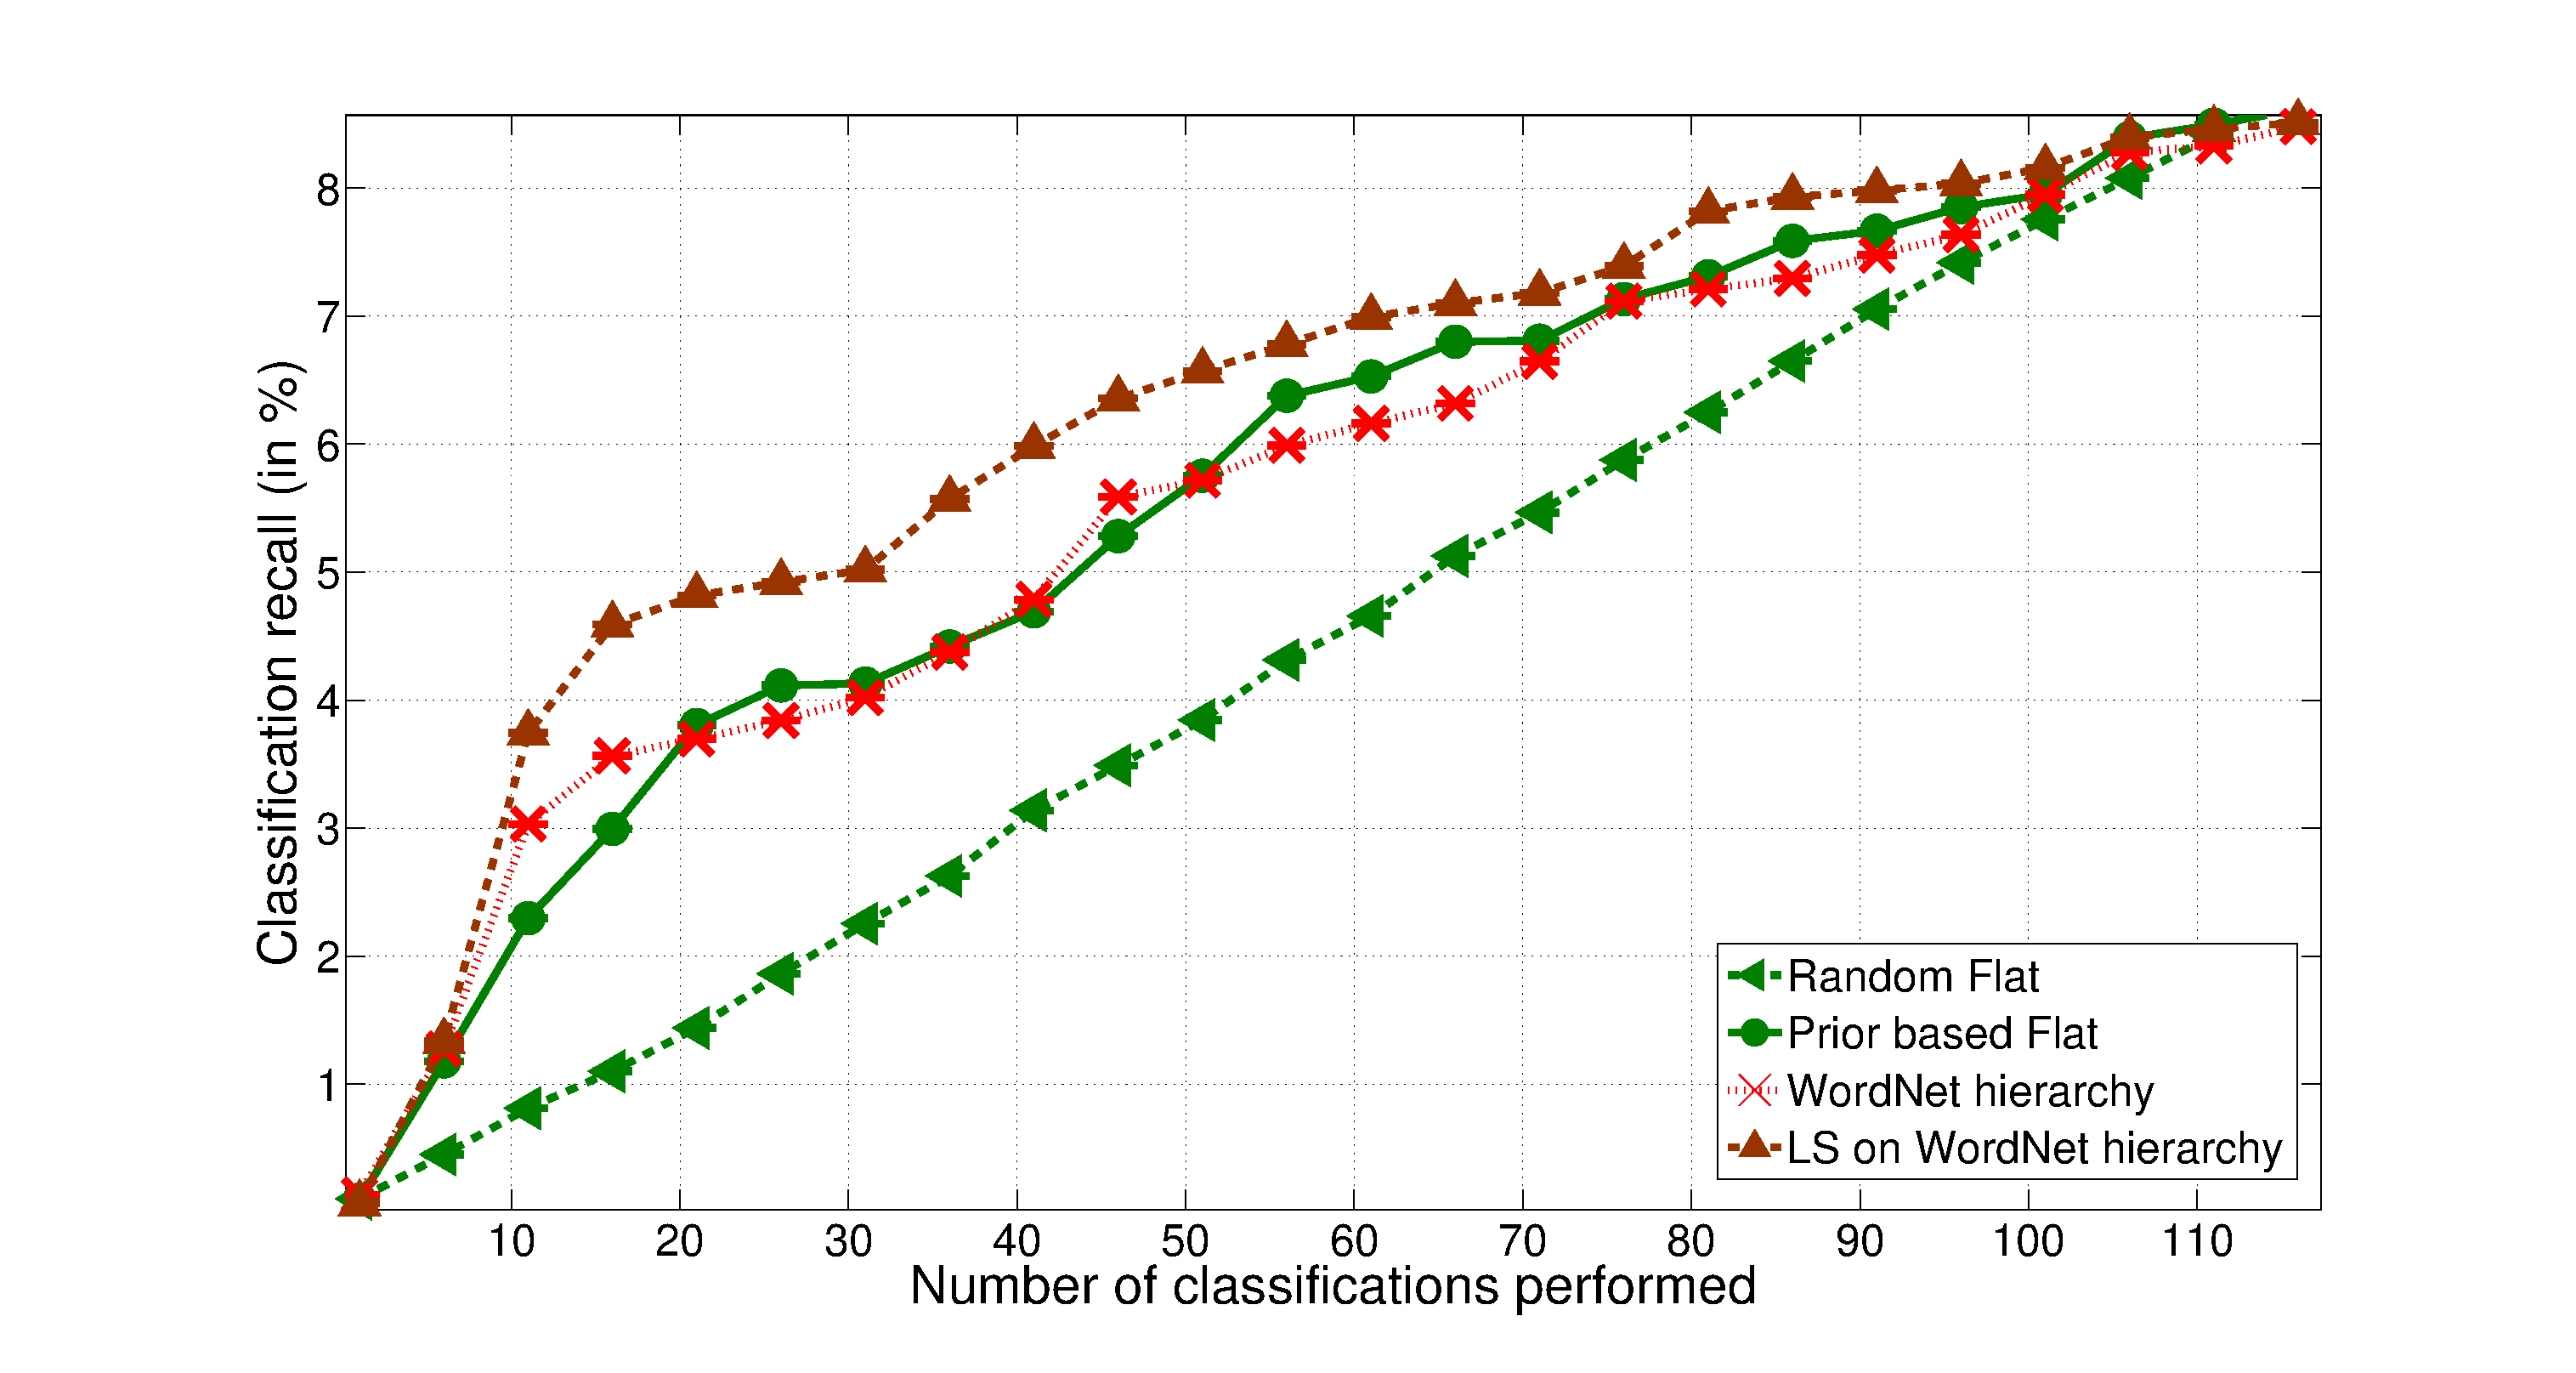
\includegraphics[width=\linewidth]{FastTagPredFWS117topK}
%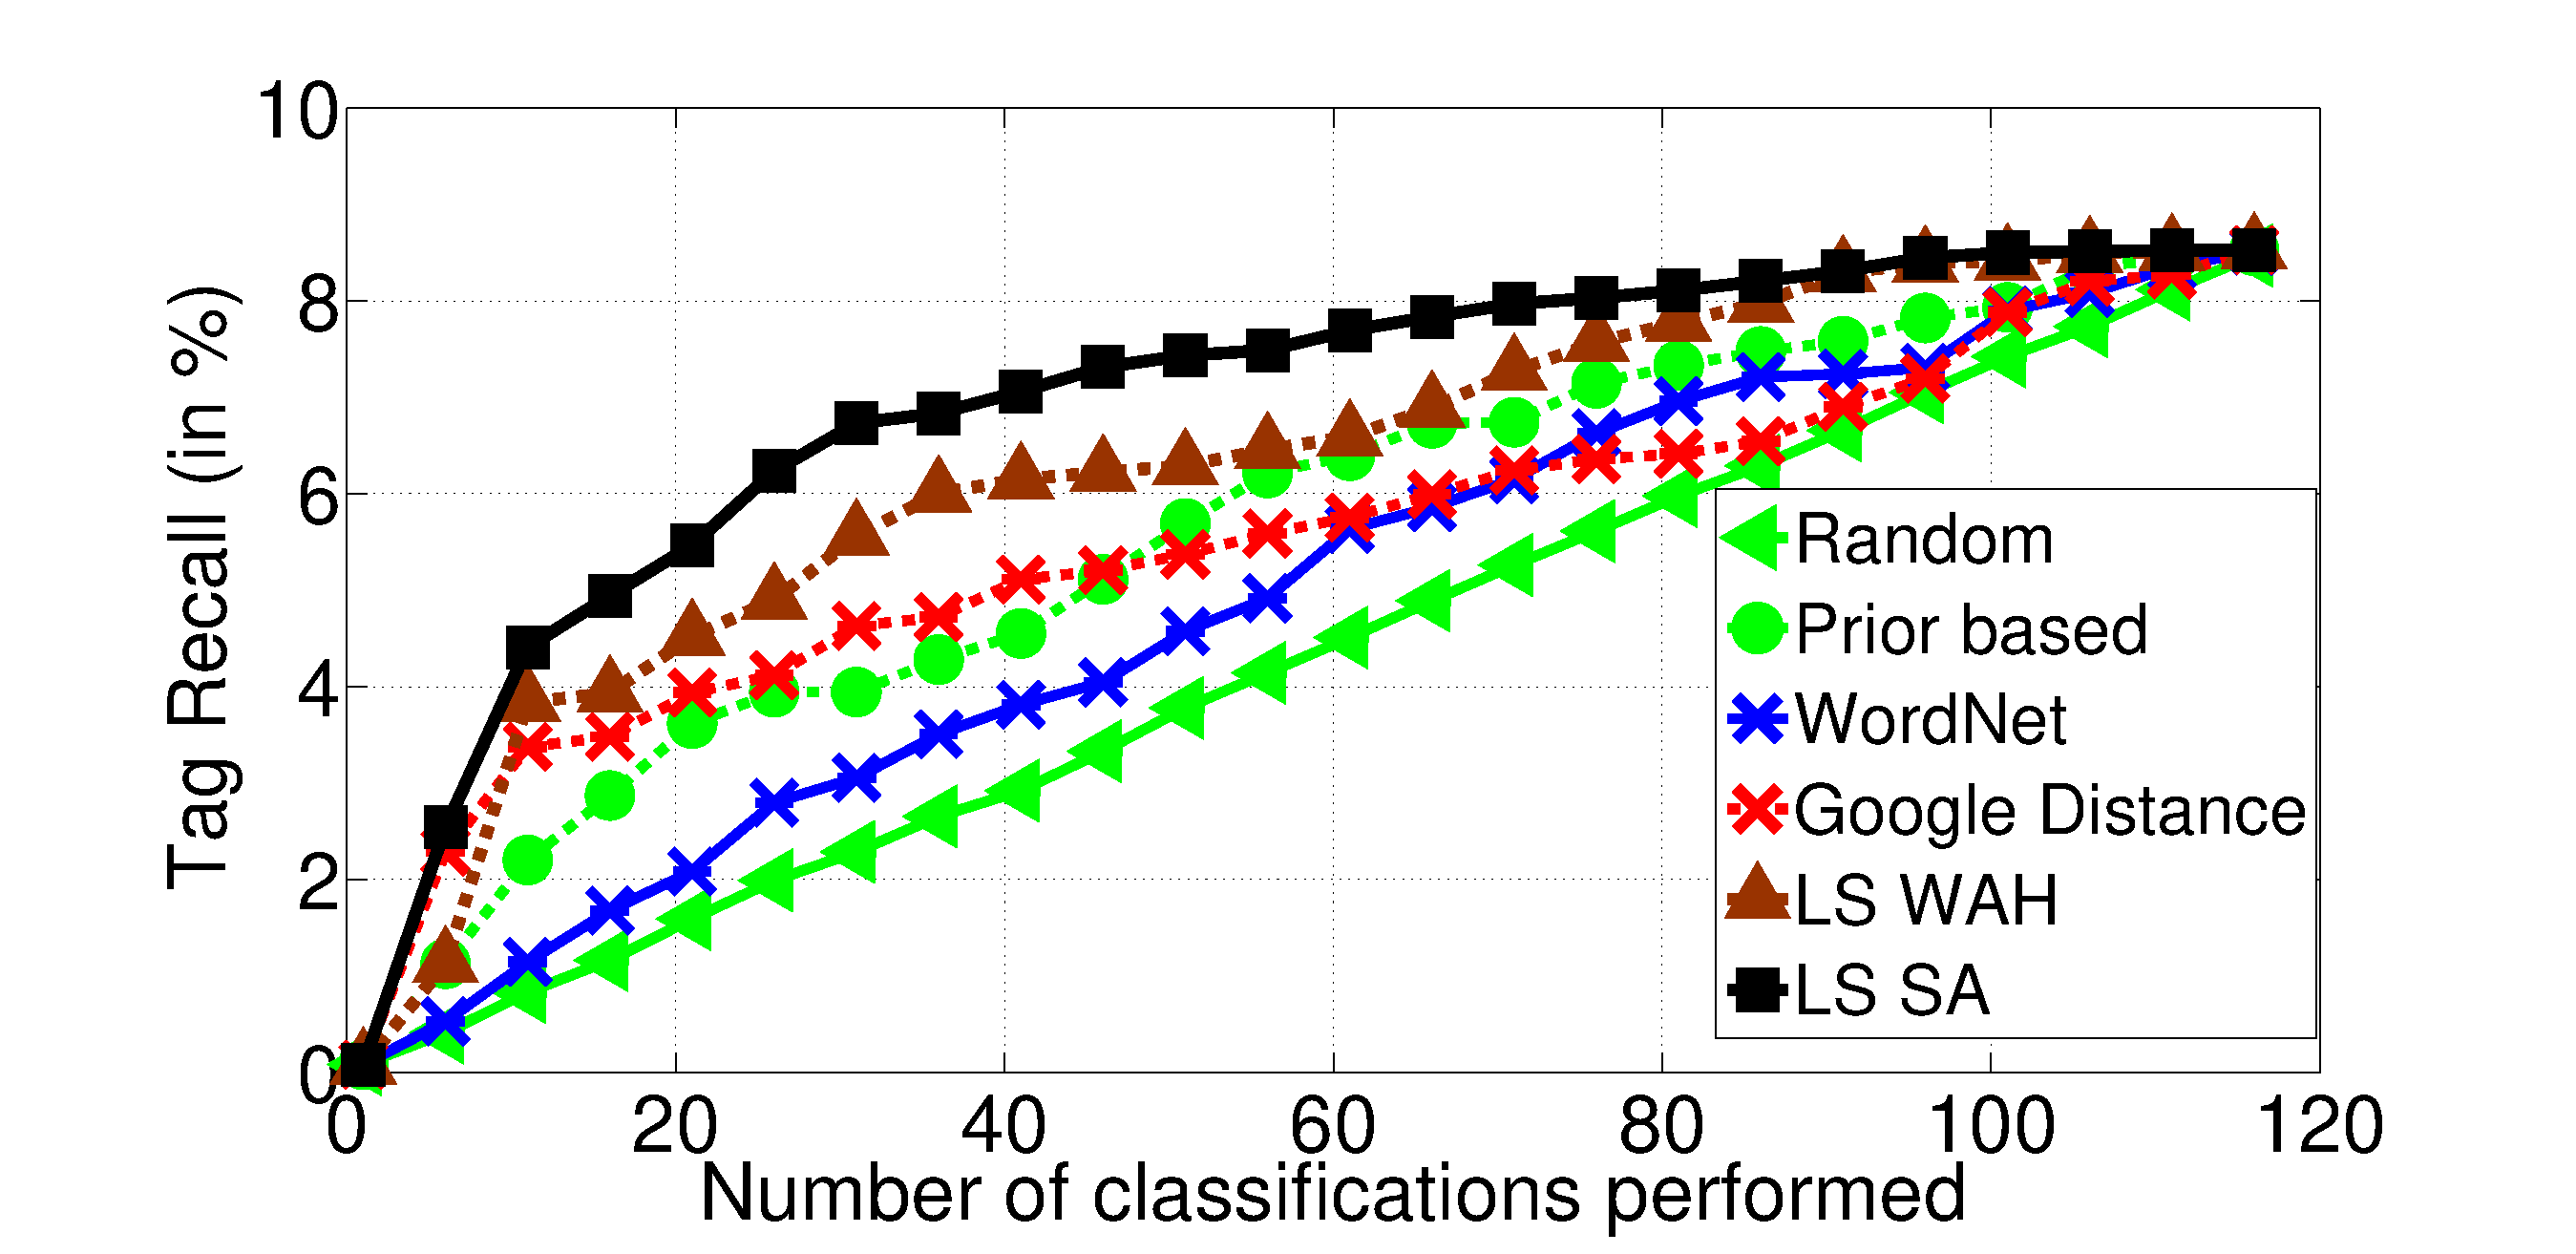
\includegraphics[width=\linewidth]{FWSFastTP_journal.eps}
\centering
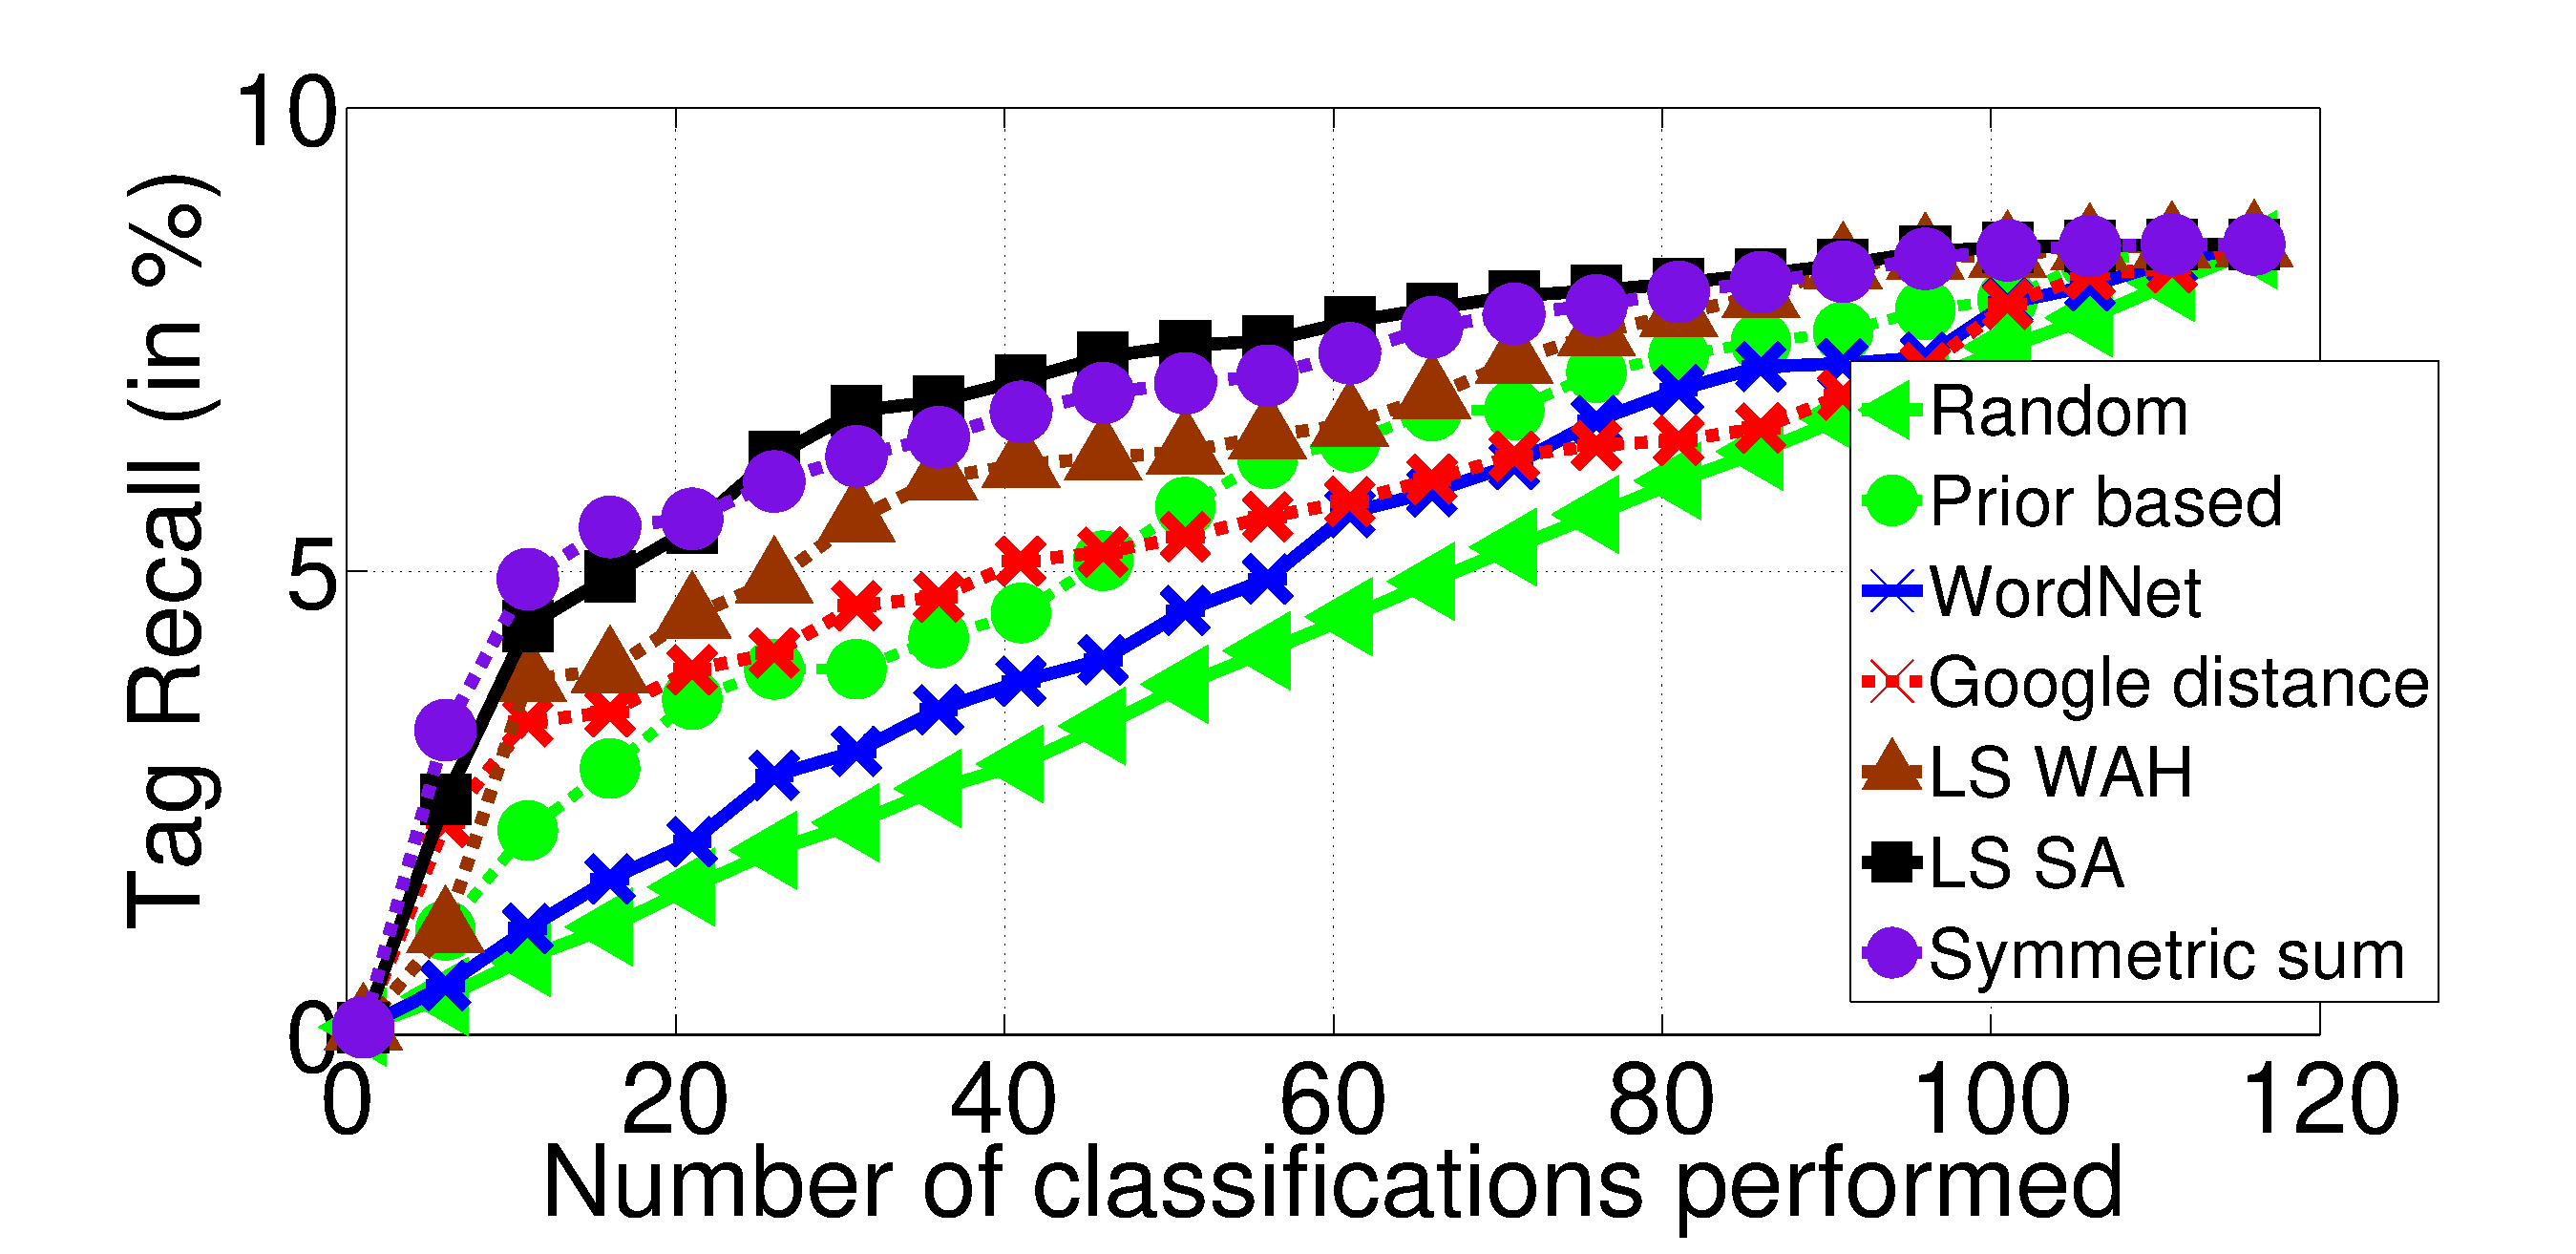
\includegraphics[width=0.65\linewidth]{TagTree/RebuttalFlickrFastTP}
\caption{\hl{Tag Recall obtained with respect to number of classifications performed for Flickr corpus. $\theta$ is chosen to  be 0.5.} } 
\label{fig:EfficientTagPredGraphFlickr}
\end{figure}
\begin{figure}[!htp]
%\epsfig{width=10cm,figure=FastTagPredFWS117topK.eps}
%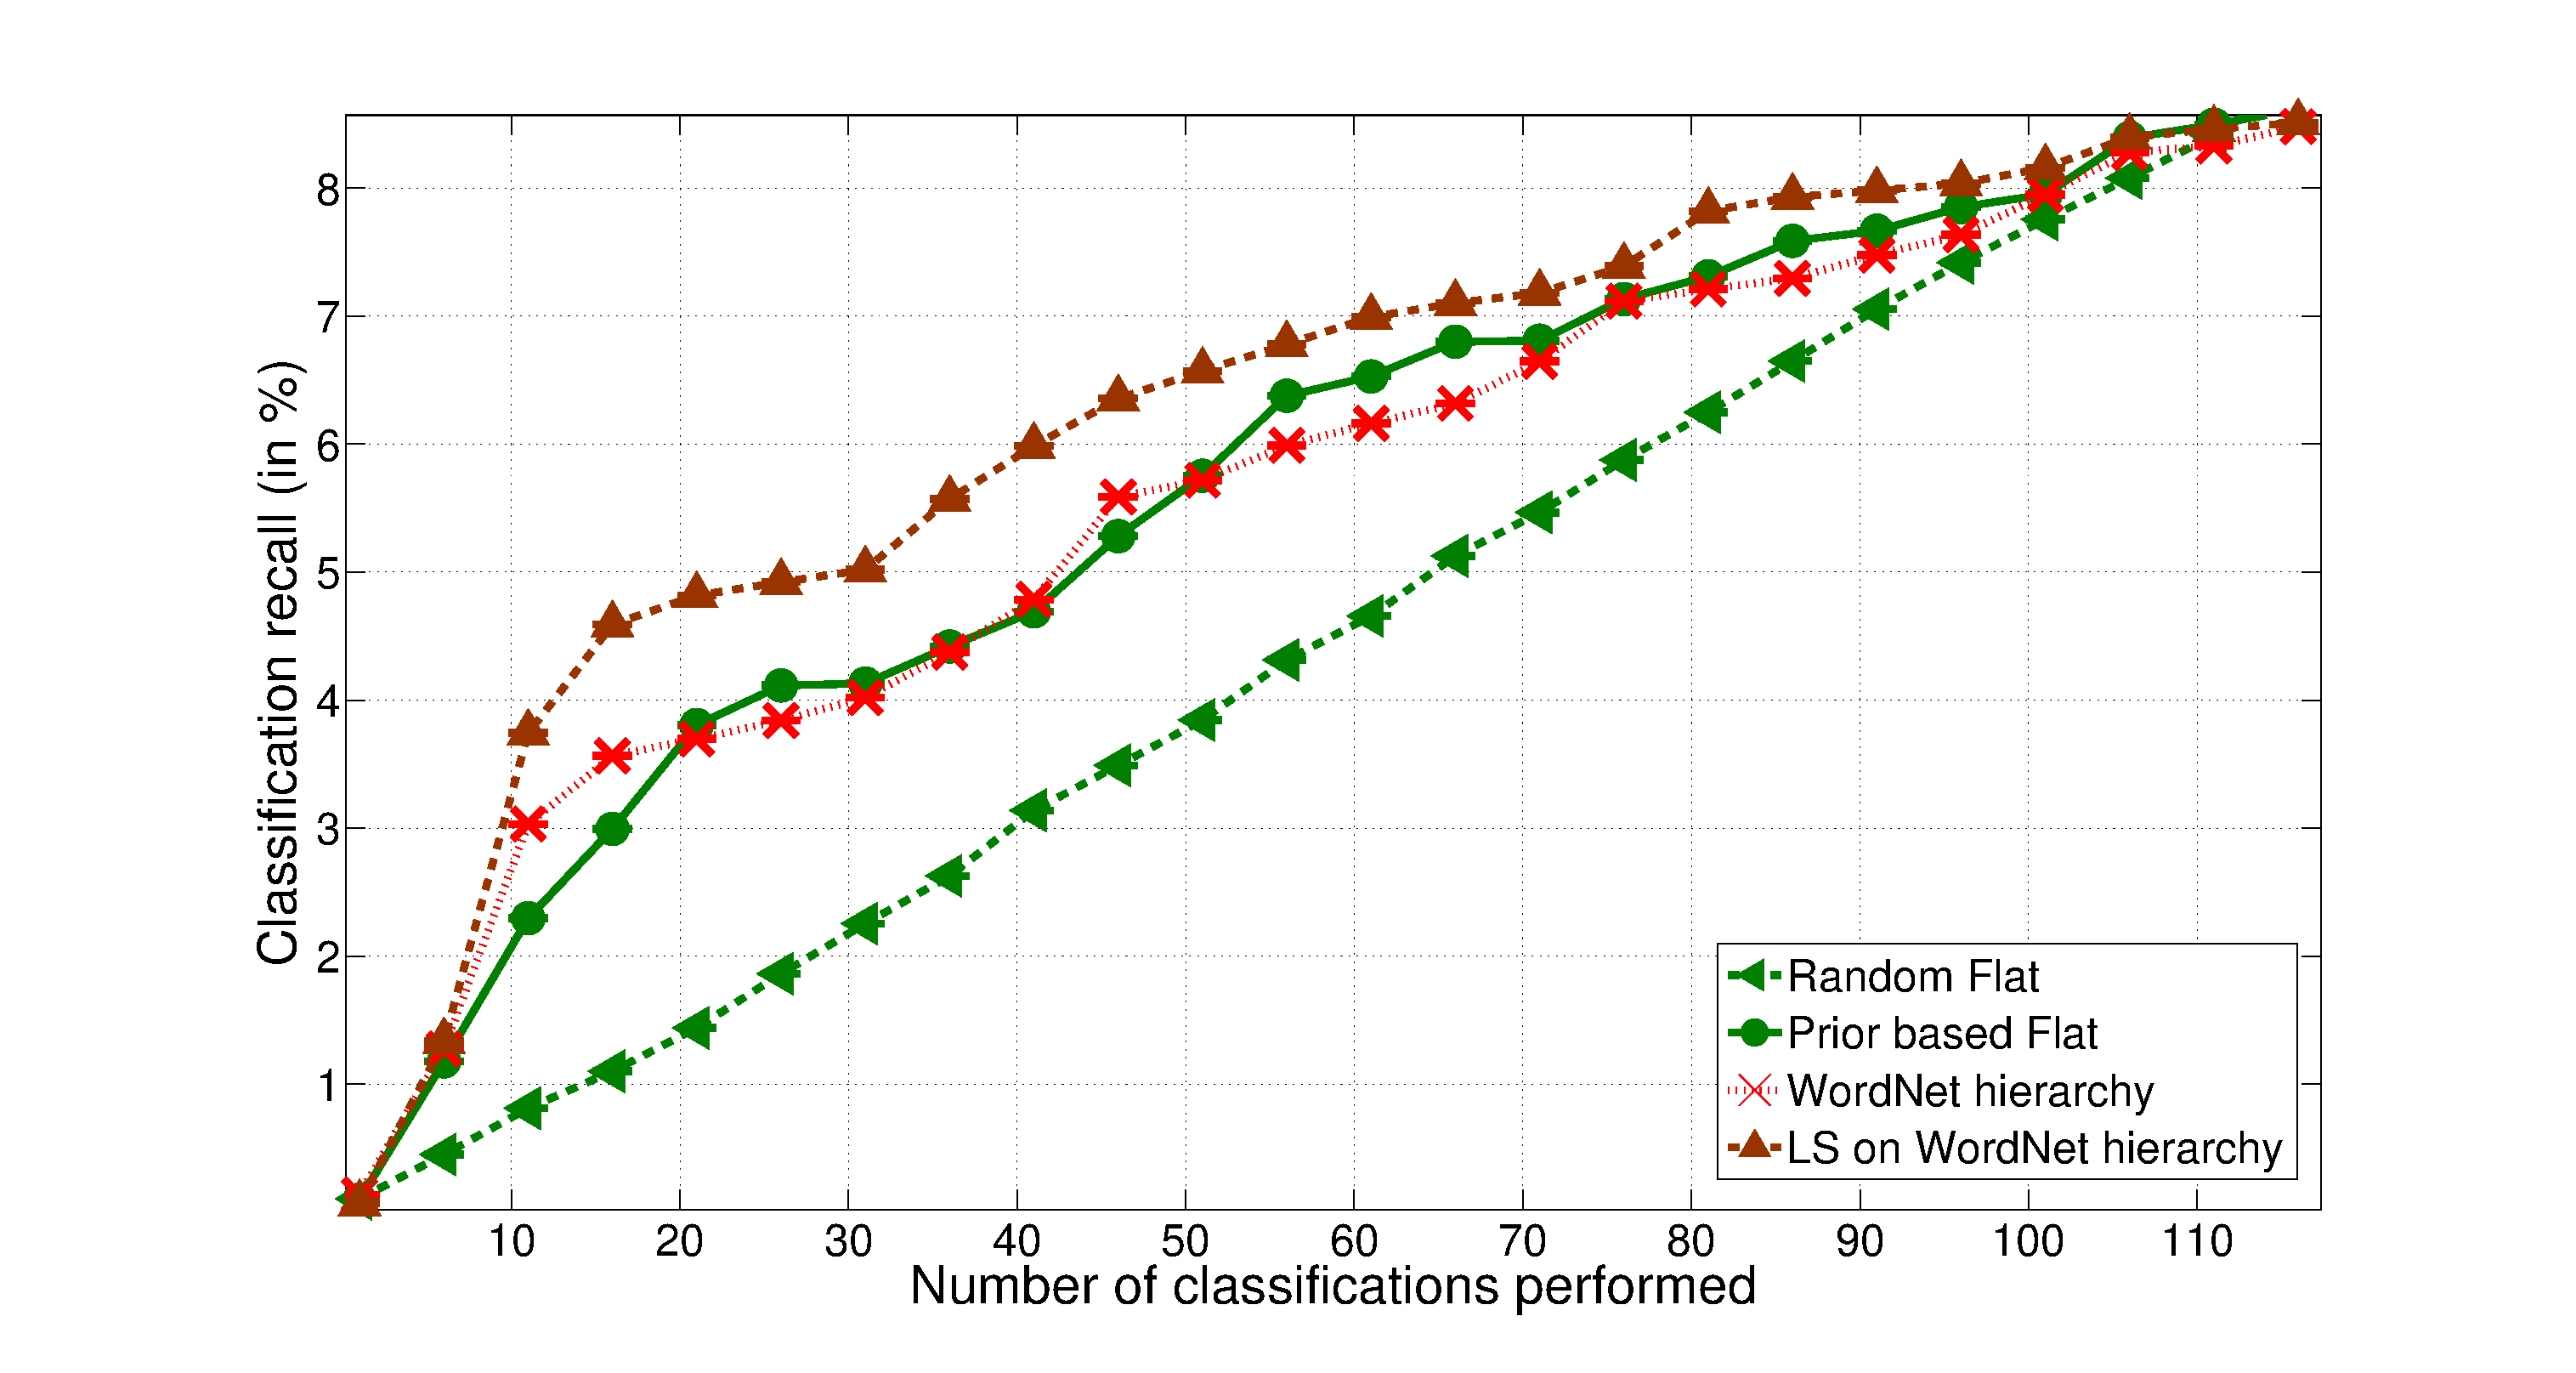
\includegraphics[width=\linewidth]{FastTagPredFWS117topK}
%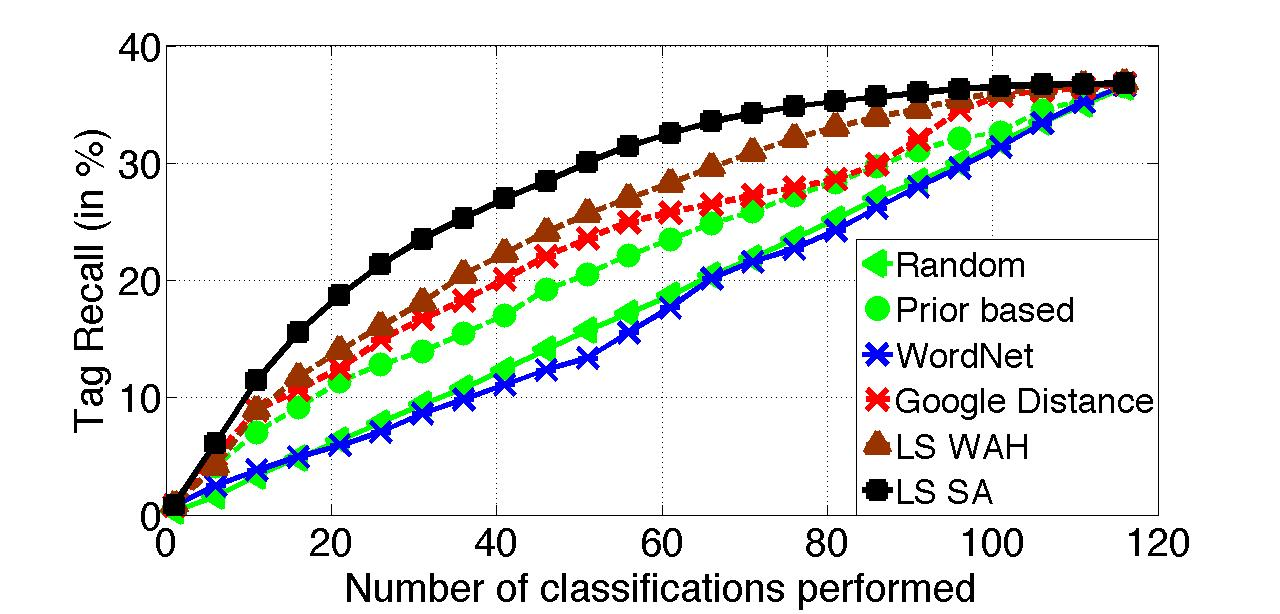
\includegraphics[width=\linewidth]{Journal_FastTagPredResults_LowerThreshMinpt5}
\centering
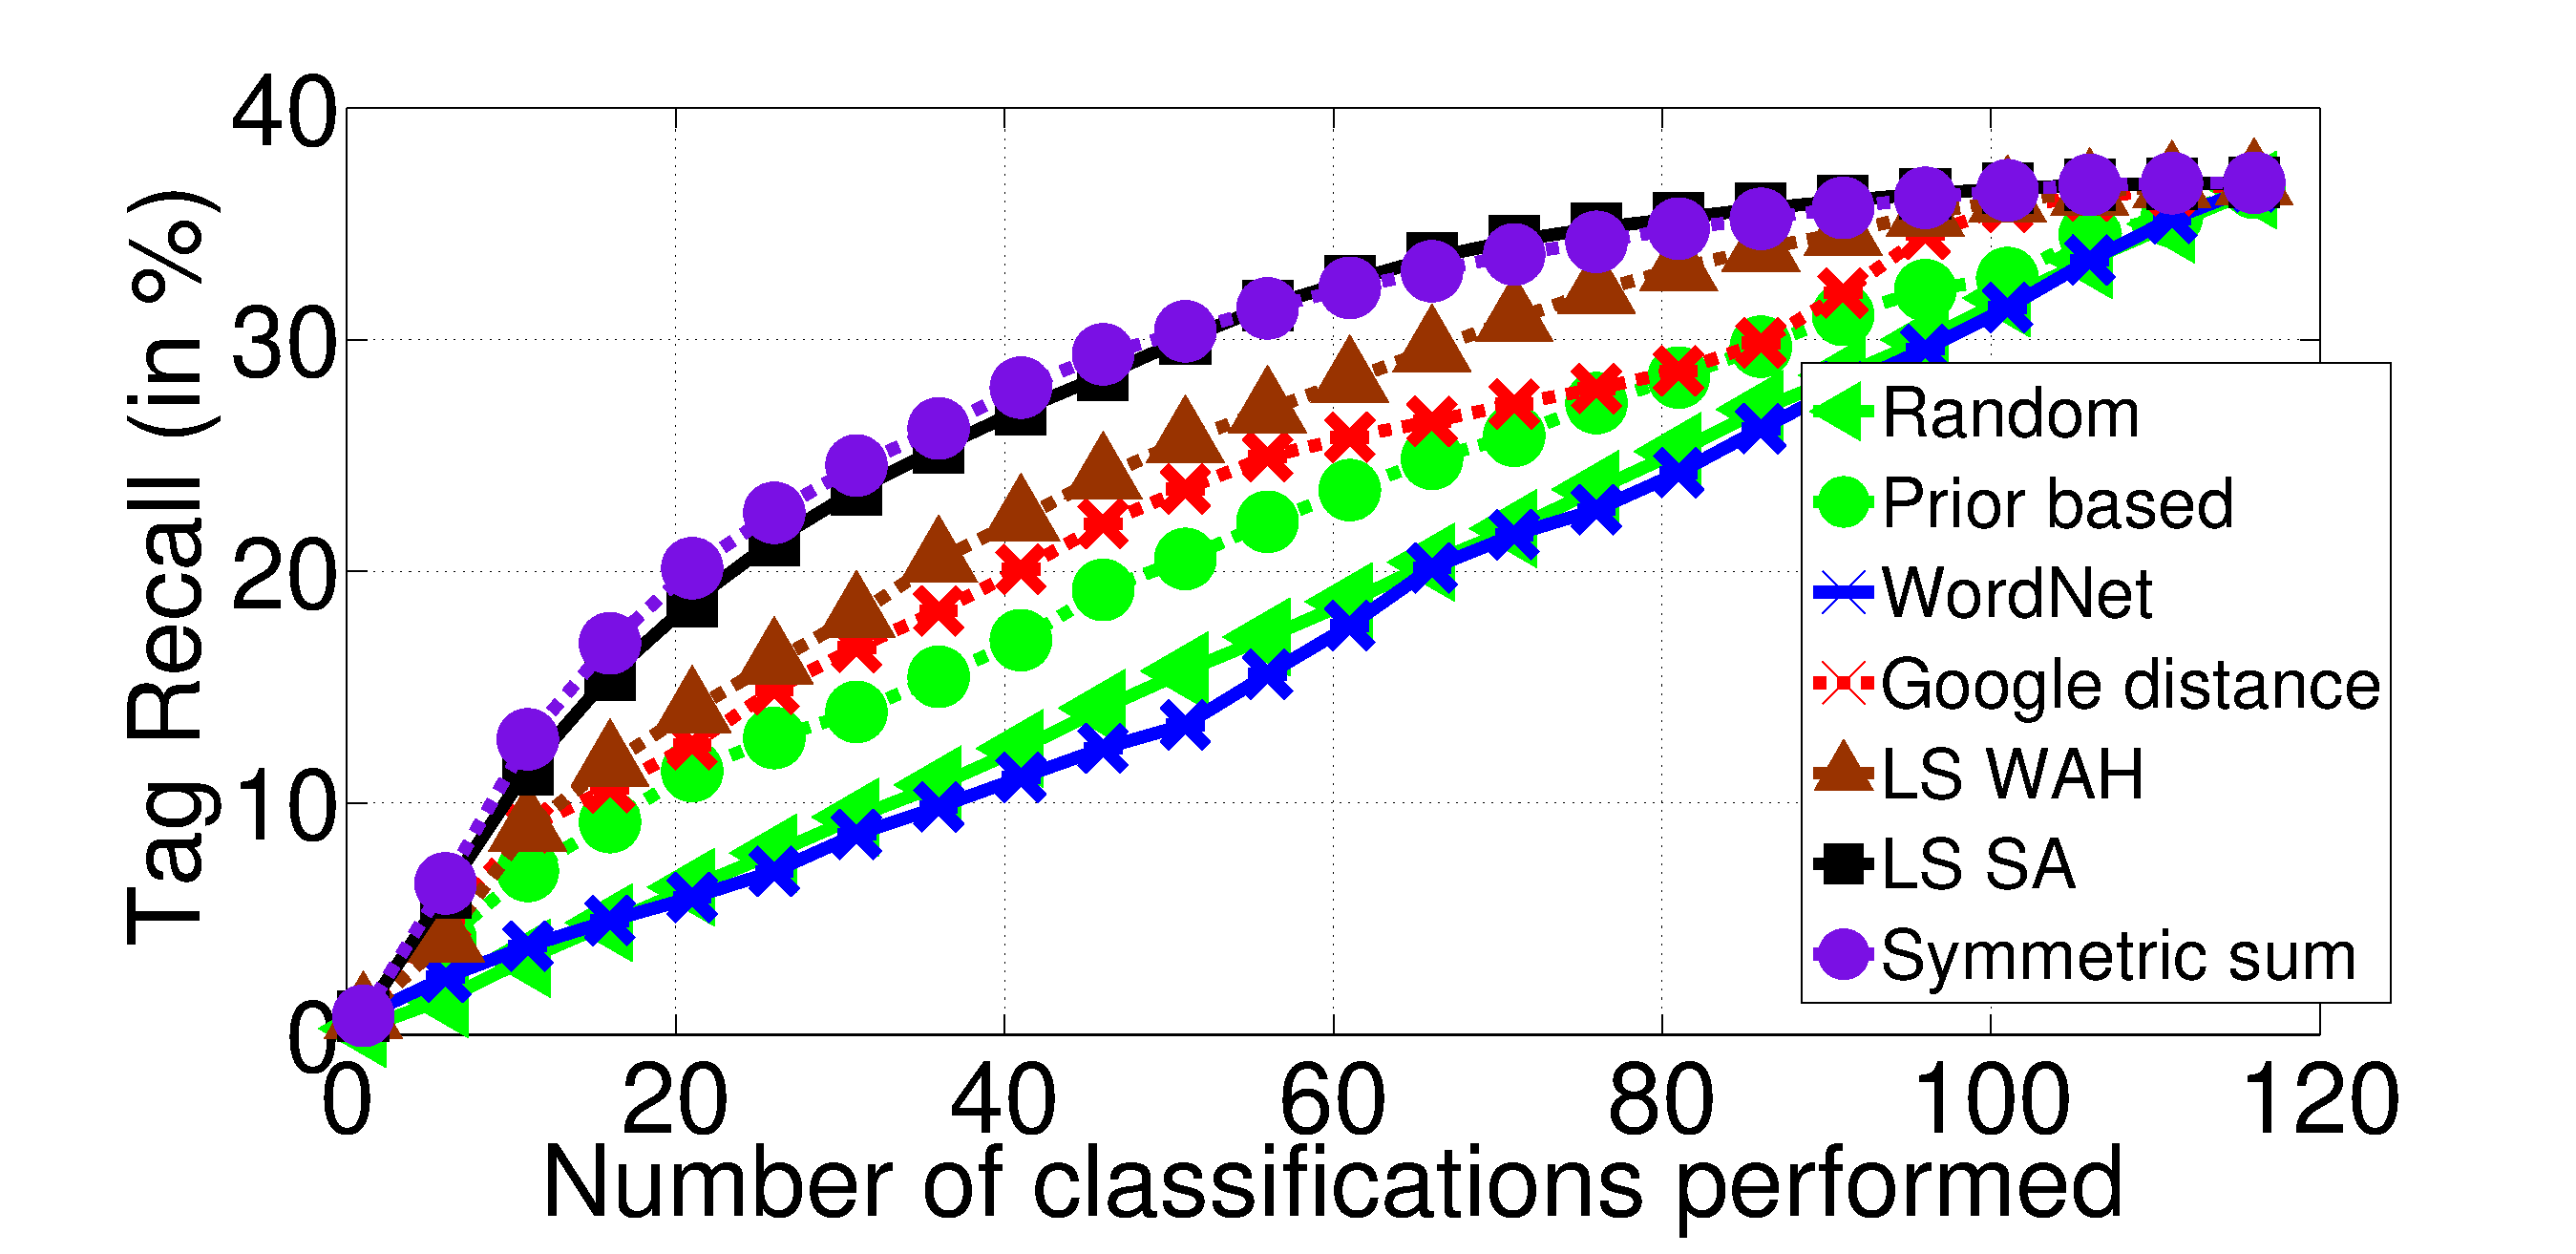
\includegraphics[width=0.65\linewidth]{TagTree/Rebuttal_FWS_Fast_LOWER}
\caption{\hl{Tag Recall obtained with respect to number of classifications performed for Flickr corpus. $\theta$ is chosen to be 0.33. } }
\label{fig:EfficientTagPredGraphFlickrLower}
\end{figure}
\begin{figure}[!htp]
%\epsfig{width=10cm,figure=FastTagPredGWS118topK.eps}
%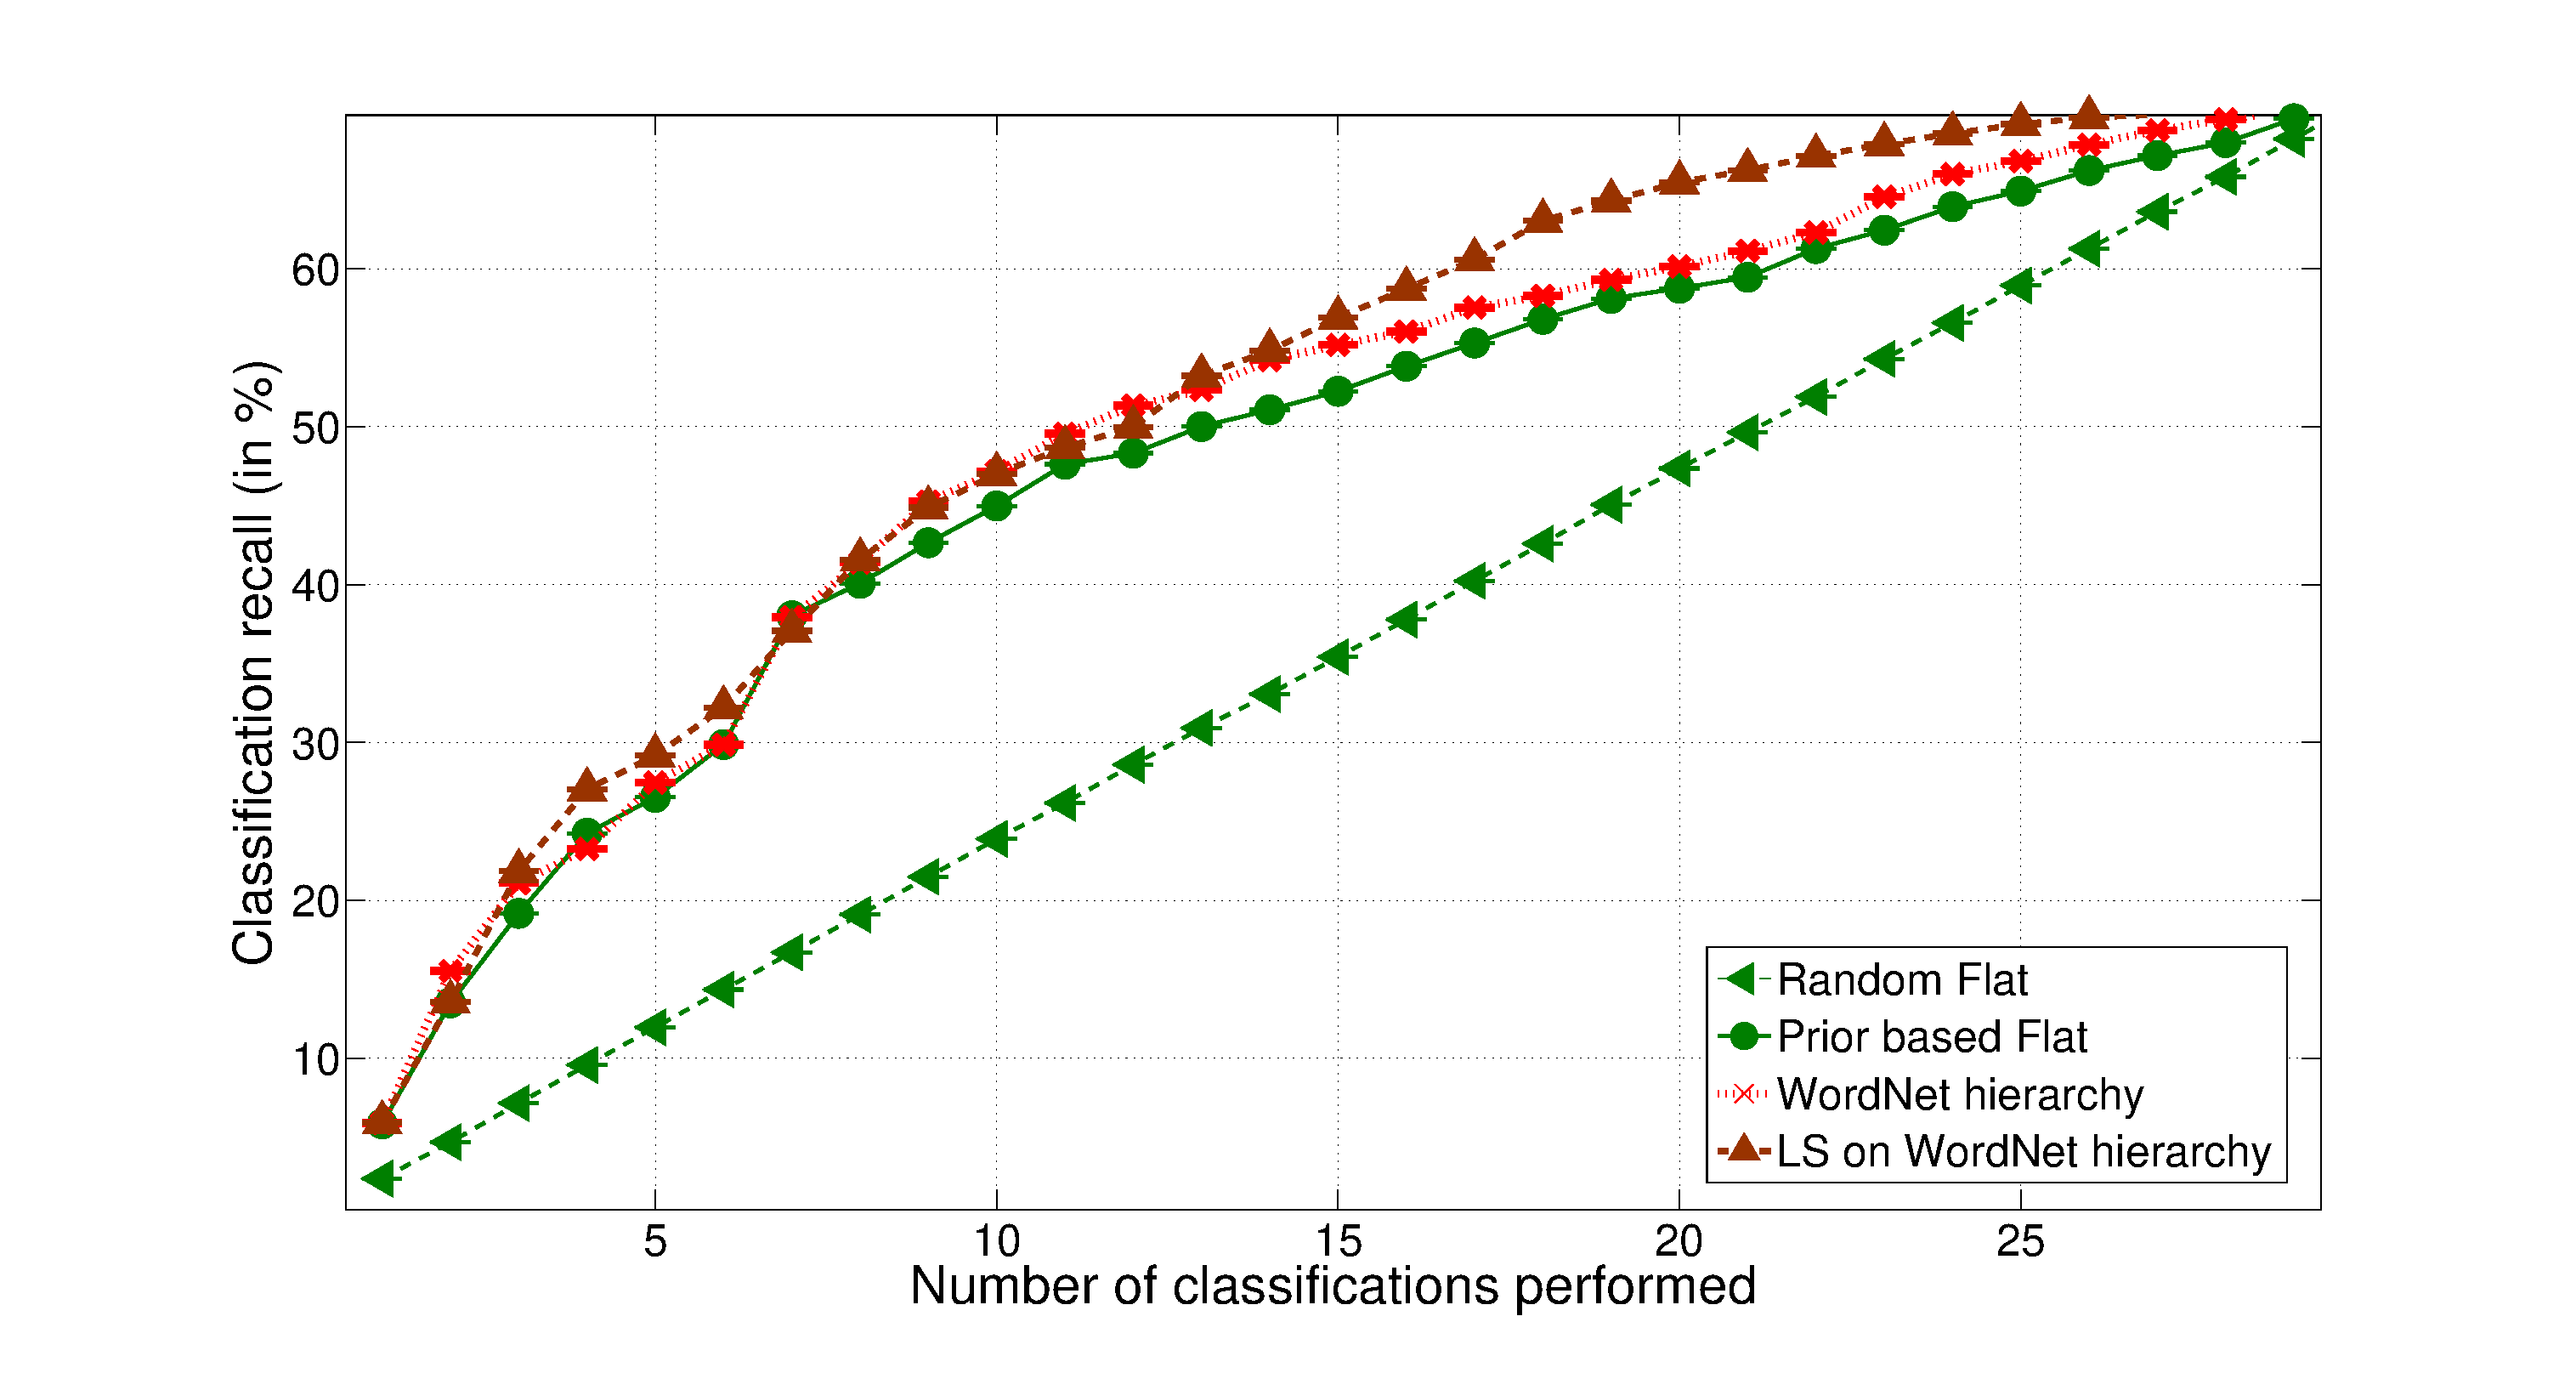
\includegraphics[width=\linewidth]{FastTagPredGWS118topK}
%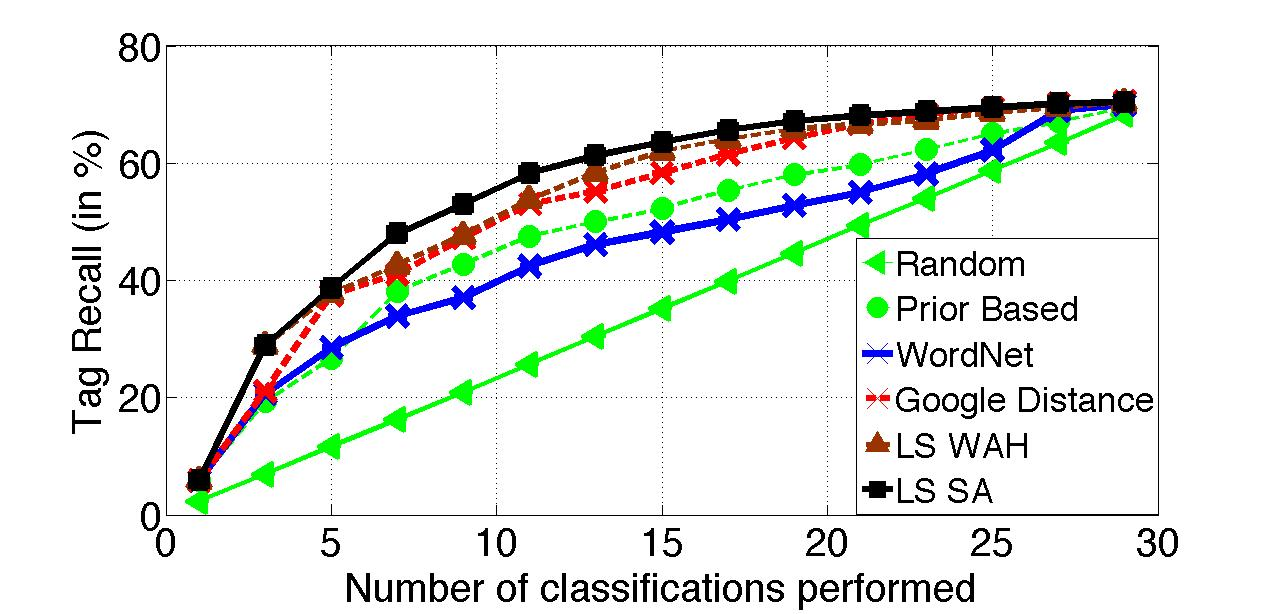
\includegraphics[width=\linewidth]{GWS30_FastTP_journal2}
\centering
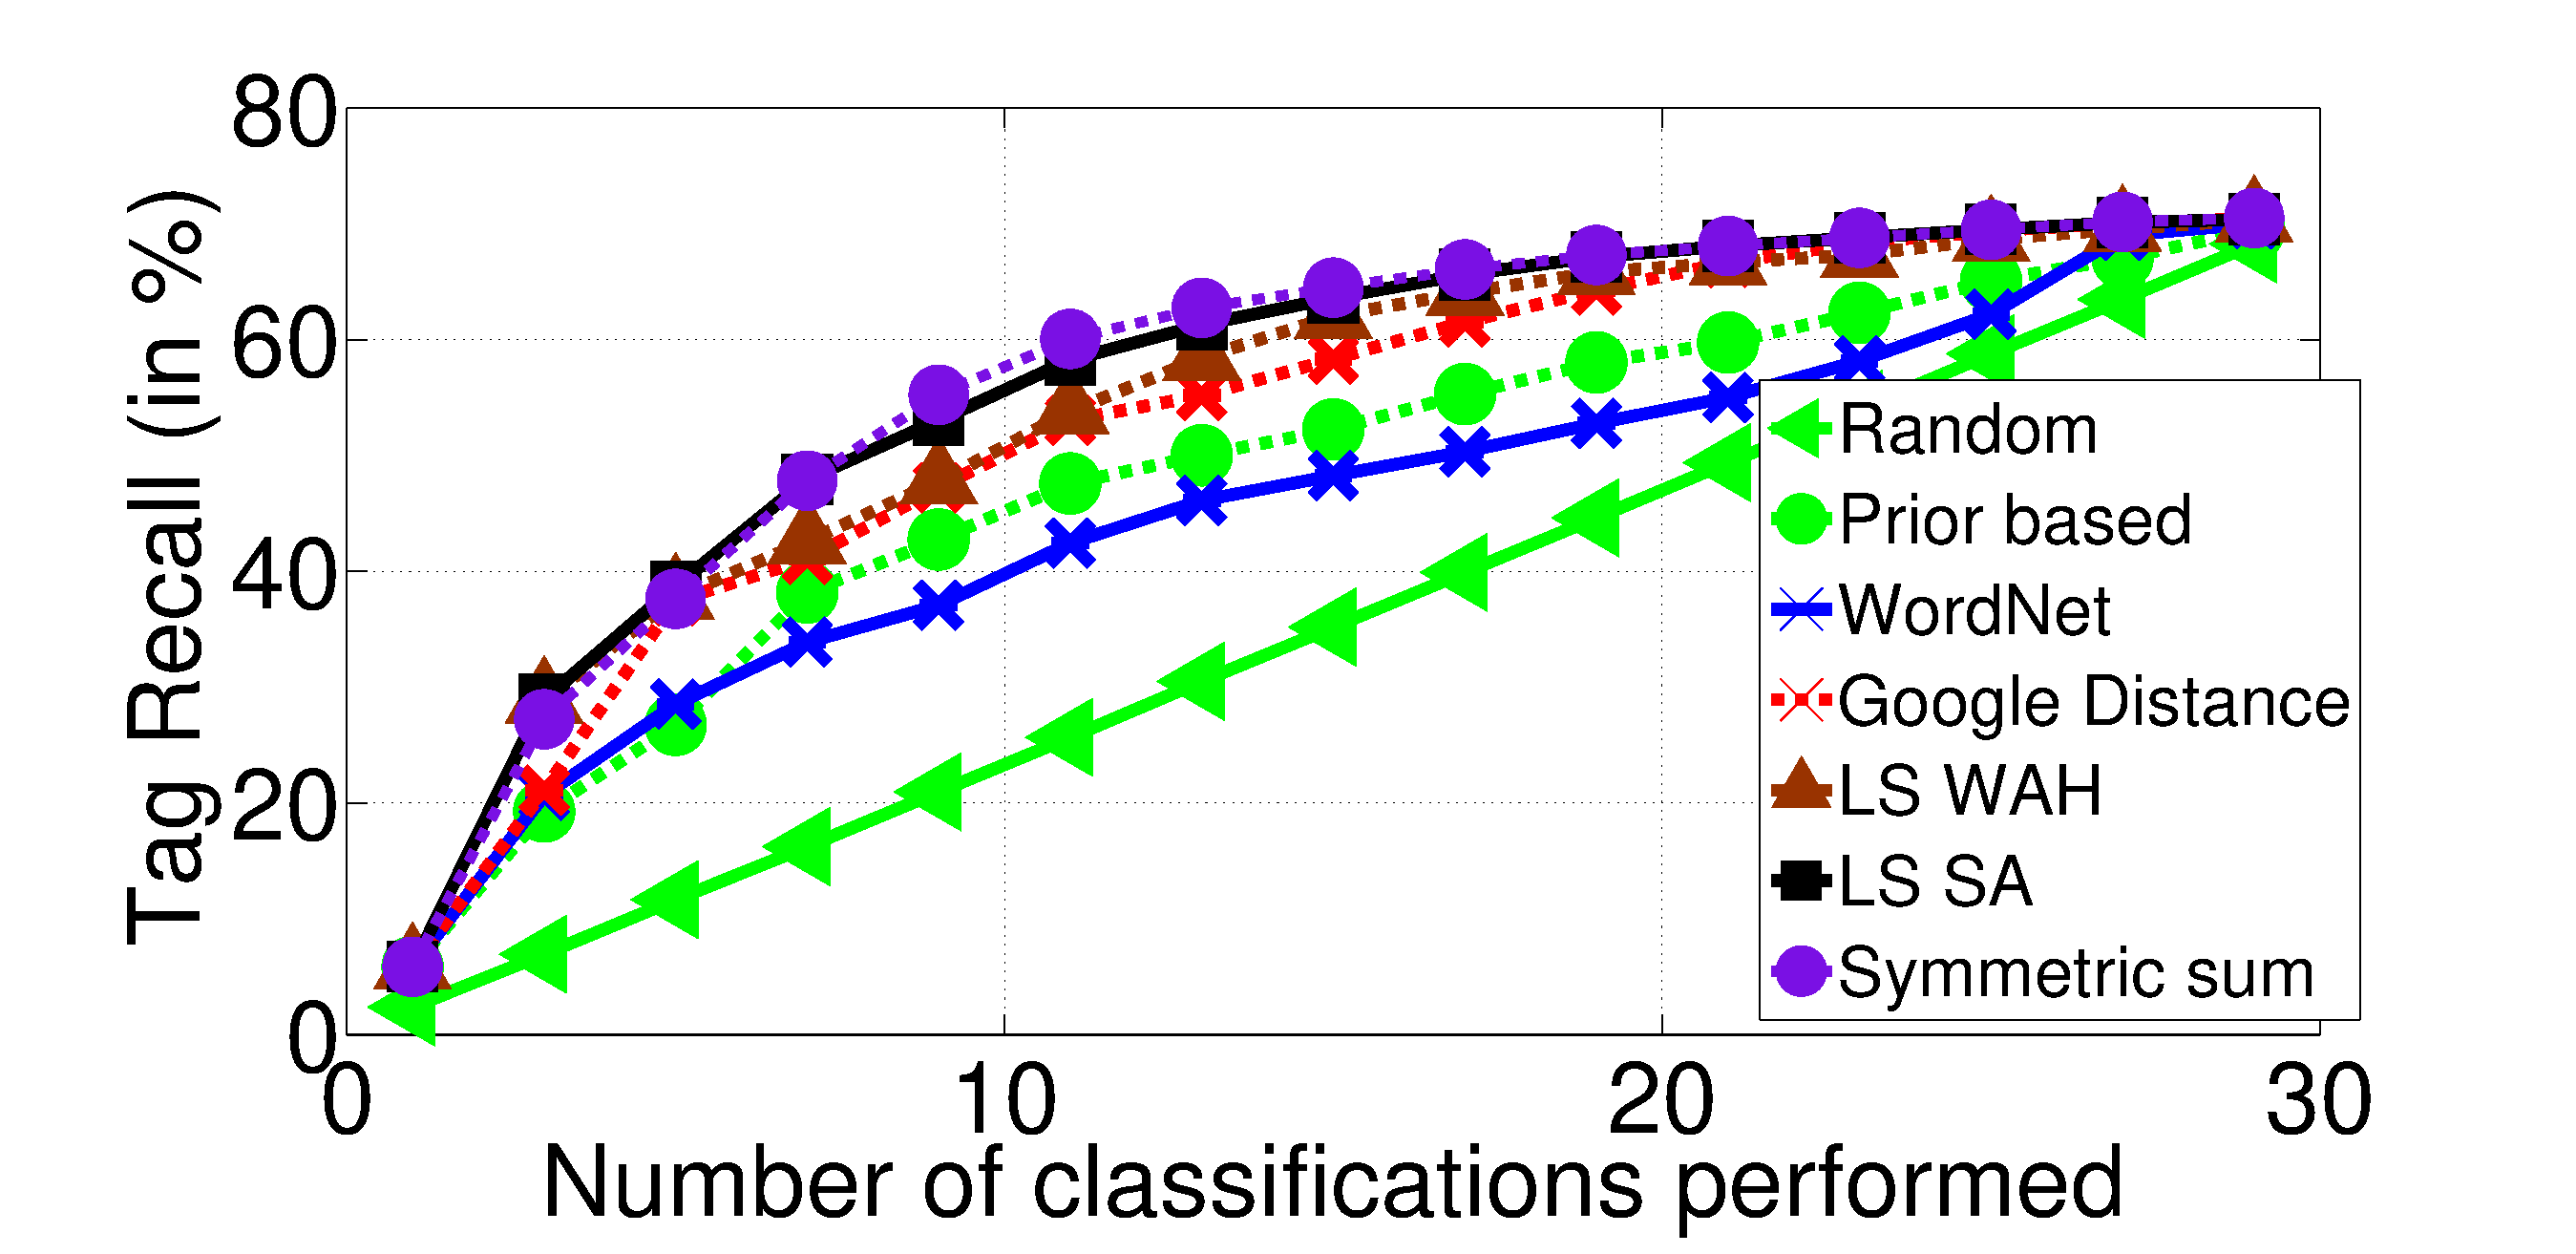
\includegraphics[width=0.65\linewidth]{TagTree/Rebuttal_FastTP_GWS}
\caption{\hl{Tag Recall obtained with respect to number of classifications performed for Stock images corpus. $\theta$ is chosen to  be 0.5. }}  
\label{fig:EfficientTagPredGraphGetty}
\end{figure}

\section{Robustness Analysis} \label{sec:Robustness}
We provide an analysis of the robustness of the proposed approach for constructing ontological tag trees. \hl{For the purpose of this section, we refer to the resource tag data using which the tag tree is constructed, as training data. The resource tag data over which the constructed tag tree is tested for evaluation purpose, is referred to as the test data}. \hl{As seen in Section {\ref{sec:Expts}}, the LS-SA method has consistently outperformed LS-WAH across different corpora and for both data-driven tasks}. Therefore, in this section we only study the robustness of the LS-SA method, i.e., the proposed local search based approach using Similarity Approximation based objective function (\ref{eq:ObjFnSimApprox}). In order to evaluate the constructed tag trees under various scenarios, we provide evaluation using tag prediction task as detailed in Section~\ref{subsec:TagPred}. \hl{Annotated image corpora are used for this purpose.} We study the robustness of proposed approach with respect to label noise, difference between training and test data, and the size of training data. These are discussed in detail below. 
\subsection{Robustness to Label Noise in Training Data}
\label{sec:RobustNoise}
\hl{As described in Section~{\ref{sec:Introduction}}, a vast majority of the user generated data available over the Internet has noisy labels (tags) associated with the resources}. We study the effect of different degrees of label noise on the tag tree constructed from such a noisy corpus. Fundamentally, we attempt to understand how robust the proposed tag tree construction approach is, to different degrees of label noise. We also attempt to answer questions such as - how much noise is too much for tag tree construction? 
\begin{figure}
%\epsfig{width=10cm,figure=VaryFWSorNoisewithGWSTPAccVary.eps}
%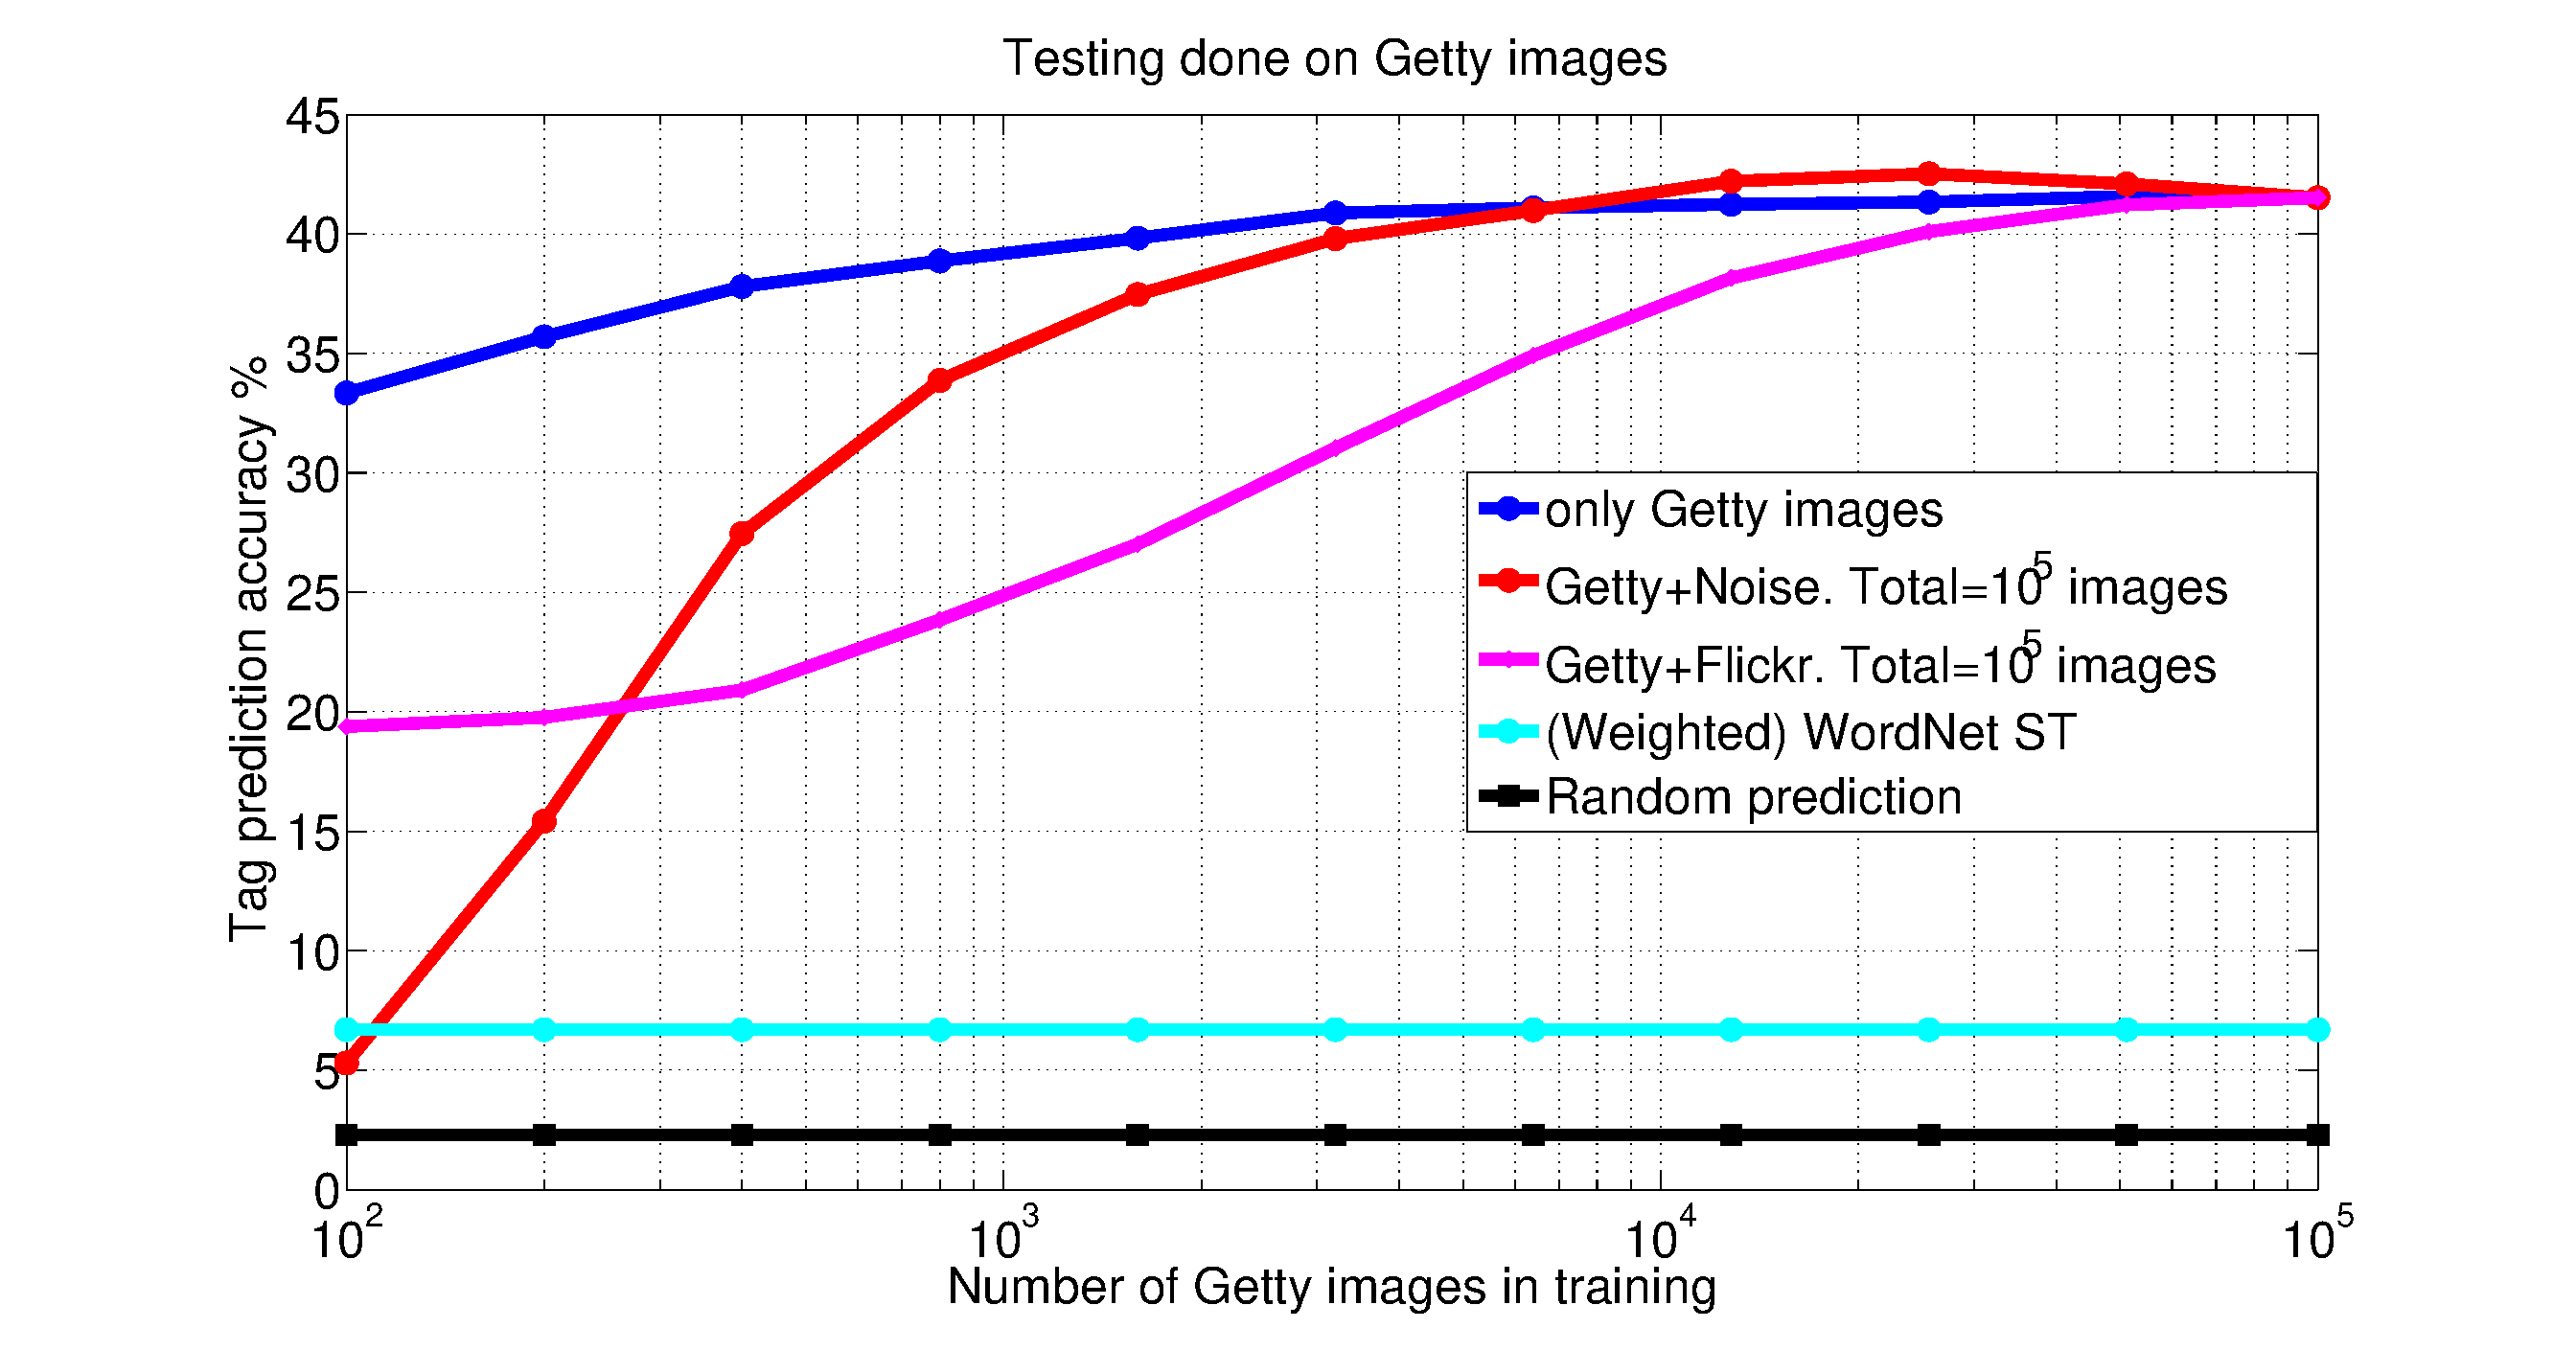
\includegraphics[width=\linewidth]{VaryFWSorNoisewithGWSTPAccVary}
\centering
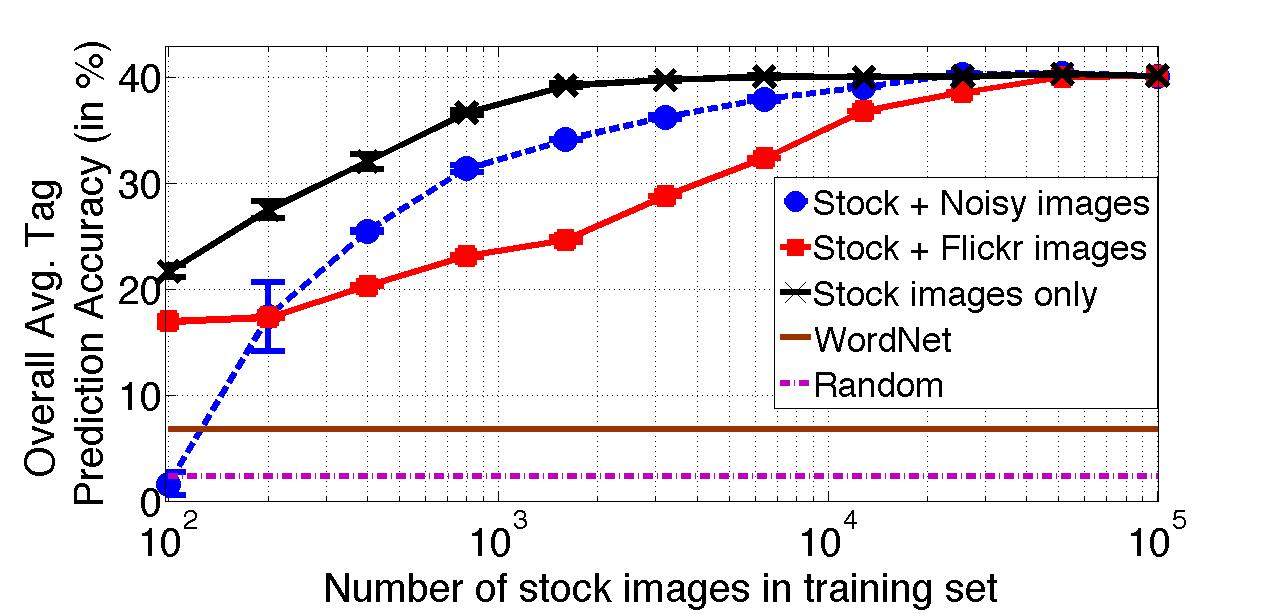
\includegraphics[width=0.65\linewidth]{TagTree/journal_RobustnessFig}
\caption[Robustness analysis using Overall Tag Prediction Score (in \%) obtained by proposed approach in Section~\ref{sec:TagPredUsingGraph}. ]{Overall Tag Prediction Score (in \%) obtained by proposed approach in Section~\ref{sec:TagPredUsingGraph}. The training set used to construct an ontological tag tree is formed by using certain number of stock images, with A) Flickr images, or B) noisy images, or C) none. Testing of the constructed tag tree is done on images of stock photos only. For comparison, the Overall Tag Prediction Accuracies for Random method, and WordNet method (as outlined in Section~\ref{sec:comparison}) are also provided. } 
%\vspace{-5mm}
\label{fig:AddNoiseTrainingData}
\end{figure}

We work with stock image corpus since stock images are professionally curated and have little to no label noise, thus providing a better control on the amount of noise in the experimental data. We select top 150 tags (keywords) from this corpus and remove those that do not occur in Flickr or in WordNet. This gives a set $\mathcal{T}$  of 108 tags. Each stock image has on an average 3 tags amongst $\mathcal{T}$. A total of 100,000 stock images are used in training set and 50,000 stock images in the test set. In order to simulate varying degrees of label noise in training set, we replace stock images in the training data with artificially created images with noisy tags. The total number of training images (stock images and noisy images) is kept constant at 100,000. The artificially created noisy images are defined as images having exactly 3 randomly chosen tags from $\mathcal{T}$. The test set is not varied.  Fig. ~\ref{fig:AddNoiseTrainingData} shows the variation of Overall Tag Prediction Accuracy (\%) as defined in Section \ref{subsec:TagPred}, with number of images that were from stock images in the training set. It can be seen that even with 87.2\% noisy images in the training set, the performance of the constructed tag tree (39\%) is very close to the performance when there are no noisy images at all (40\%). Even when 99.2\% of the images in training set are noisy, the Overall Tag Prediction Accuracy is 31.4\%. An explanation for such performance even at high levels of noise is that the noisy images have uniformly random distribution of tags. The overall effect of adding noisy images to a corpus can be understood as adding certain intensity of white noise to the co-occurrence counts between tags. Unless the noise intensity dominates the corpus statistics, the relative order of pair-wise connections between tags remains fairly unchanged. In other words, since the noisy images have no strong biases towards specific tag-pairs, the performance of tag trees constructed using such a hybrid training set is not severely affected. 

\subsection{Robustness to Difference between Training and Test Data}
\label{sec:RobustDifference}
In several machine learning applications, the data over which a model is trained has certain amount of distributional difference as compared to the data over which it is tested. Looking at the construction of tag tree as model training, the degree to which a tag tree will be effective on a test set is a function of the difference between the test set and the training set using which the tag tree is constructed. Here we study how the performance of a tag tree varies for different degrees of difference between the training and the test sets. We utilize the same stock images corpus as used in Section~\ref{sec:RobustNoise}. In order to vary the difference between training and test sets, we replace varying number of stock images in training set with images from Flickr corpus (Section~\ref{sec:Datasets}). The total number of images (stock images and Flickr images) used for training of tag tree is kept constant at 100,000. Fig.~\ref{fig:AddNoiseTrainingData} shows the variation of Overall Tag Prediction Accuracy (\%) with number of images that were from stock images in the training set. It is interesting to note that for the same number of stock images, adding completely noisy images leads to better performance than adding Flickr images. For instance, for the case when 99.2\% of training images are from Flickr, performance of the constructed tag tree (23.1\%) is seen to be substantially worse than when 99.2\% of training images are noisy (31.4\%). The reason for this is that the tag distribution in Flickr corpus is not random, unlike in the case of noisy images. As a result, there are strong relationships between tags in Flickr corpus that are absent in stock image corpus. Constructing a tag tree on such a hybrid corpus attempts to capture corpus statistics of varying numbers of Flickr images and stock images, and in the process, is less effective at capturing the relationships that were present in the test data that has only stock images. 

\subsection{Size of Training Data}
\label{sec:RobustSize}
In this section, we study the effect of size of training set on construction of tag trees. Fig. ~\ref{fig:AddNoiseTrainingData} shows the variation of Overall Tag Prediction Accuracy (\%) with number of stock images in the training data. Here the size of training set is equal to the number of stock images in it and there are no Flickr images or noisy images. The performance of constructed tag tree improves with size of training data and almost saturates after certain number of training images. This is quite similar to the variation in performance of most machine learning models with the size of data over which they are trained. The performance of constructed tag tree from only 800 stock images is very close to the performance when 100,000 images are used. Even when only 100 stock images are used, the constructed tag tree performs much better than the tag trees using 100 stock images with 99900 Flickr or noisy images. Based on above, one can conclude that for the construction of ontological tag trees, it is better to use fewer training images than a larger set which is noisy or dissimilar to the test set.  
\comment{
\begin{figure}[htbp]
\centering
\begin{tabular}{p{2.2cm} p{2.2cm} p{3cm}}
\centering
\epsfig{width=2cm,height=2.8cm,figure=TagTree/figures/3569597369_690c84559a.eps} & %32965350@N00
\epsfig{width=2cm,height=2.8cm,figure=TagTree/figures/183307784_ca9034cc51.eps} & %85598619@N00
\epsfig{width=2.8cm,height=2cm,figure=TagTree/figures/180824073_fc5f017f46.eps}\\ %22768390@N00
(a){\bf holiday, island}, travel, vacation, water&
(b){\bf england, street}, building, london,uk&
(c){\bf germany, travel}, deutschland, europe, summer\\
\end{tabular}
\caption{A few examples where the local search based refinement was able to predict two of the three tags correctly, given two original tags (shown in bold). Tag prediction based on WordNet did not result in correct prediction for these examples. The Flickr owner and photo ids of these images are (32965350@N00,3569597369), (85598619@N00,183307784), (22768390@N00,180824073) respectively.}
\label{fig:examples}
\end{figure}
}
\begin{figure*}
        \centering
	\captionsetup{justification=raggedright,
	singlelinecheck=false
	}
        \begin{subfigure}[b]{0.16\textwidth}
                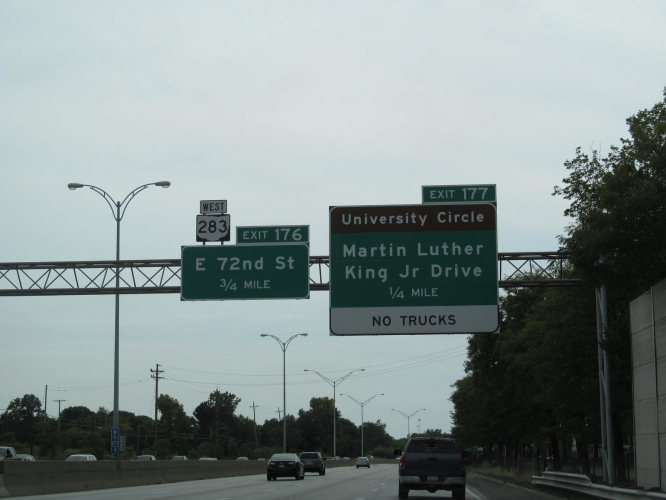
\includegraphics[width=0.8\textwidth]{TagTree/Flickrimg/777b9480-f735-3d7a-aa91-dba84cea8bf2.jpeg} 
                \caption{\textbf{Seen}: highway, road \\ \textbf{Unseen}: route, shield, sign }
                \label{fig:posex1}
        \end{subfigure}%
	\; \vline
        \; %add desired spacing between images, e. g. ~, \quad, \qquad etc.
          %(or a blank line to force the subfigure onto a new line)
        \begin{subfigure}[b]{0.17\textwidth}
                
\includegraphics[width=0.8\textwidth]{TagTree/Flickrimg/e3bb5574-1a09-32cf-9f22-1a9eb81af7c2.jpeg}
                \caption{\textbf{Seen}: austin, \\ band \\ \textbf{Unseen}: music, texas, tx }
                \label{fig:posex2}
        \end{subfigure}%
	\; \vline
        \; %add desired spacing between images, e. g. ~, \quad, \qquad etc.
          %(or a blank line to force the subfigure onto a new line)
        \begin{subfigure}[b]{0.17\textwidth}
                
\includegraphics[width=0.8\textwidth]{TagTree/Flickrimg/7c52f0a2-78ae-3b9b-9dd0-f131124750f5.jpeg}
                \caption{\textbf{Seen}: england, europe \\ \textbf{Unseen}: london, travel, uk }
                \label{fig:posex3}
        \end{subfigure}%
	\; \vline
        \; %add desired spacing between images, e. g. ~, \quad, \qquad etc.
          %(or a blank line to force the subfigure onto a new line)
        \begin{subfigure}[b]{0.16\textwidth}
                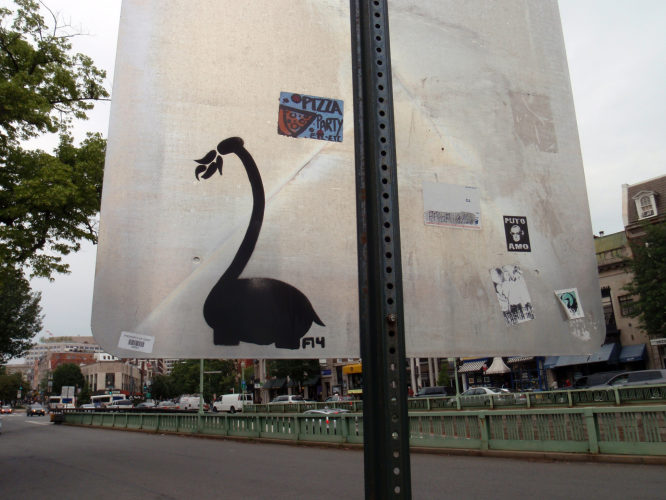
\includegraphics[width=0.8\textwidth]{TagTree/Flickrimg/b03623e7-e6cf-3e96-97cc-a7117c776614.jpeg}
                \caption{\textbf{Seen}: art, dc \\ \textbf{Unseen}: graffiti, street, washington }
                \label{fig:posex4}
        \end{subfigure}%
	\; \vline
        \; %add desired spacing between images, e. g. ~, \quad, \qquad etc.
          %(or a blank line to force the subfigure onto a new line)
        \begin{subfigure}[b]{0.17\textwidth}
                
\includegraphics[width=0.8\textwidth]{TagTree/Flickrimg/8efd5e1c-6d83-37af-91a2-1484a9d823b3.jpeg}
                \caption{\textbf{Seen}: concert, england\\ \textbf{Unseen}: london, music, uk }
                \label{fig:posex5}
        \end{subfigure}
        \caption[Example images where LS-SA method gave 100\% tag prediction accuracy when the first two tags were seen and the next three were unseen and predicted. ]{Example images where LS-SA method gave 100\% tag prediction accuracy when the first two tags were seen and the next three were unseen and predicted. The Flickr owner and photo ids of these images are (dougtone@7975042008) ,  (elchupacabra@7023118527) , (jeffwilcox@159730021) , (daquellamanera@4678084101) , (martinrp@3832812191)  respectively. } \label{fig:positiveExs}
\end{figure*}

\begin{figure*}
        \centering
	\captionsetup{justification=raggedright,
	singlelinecheck=false
	}
        \begin{subfigure}[b]{0.16\textwidth}
                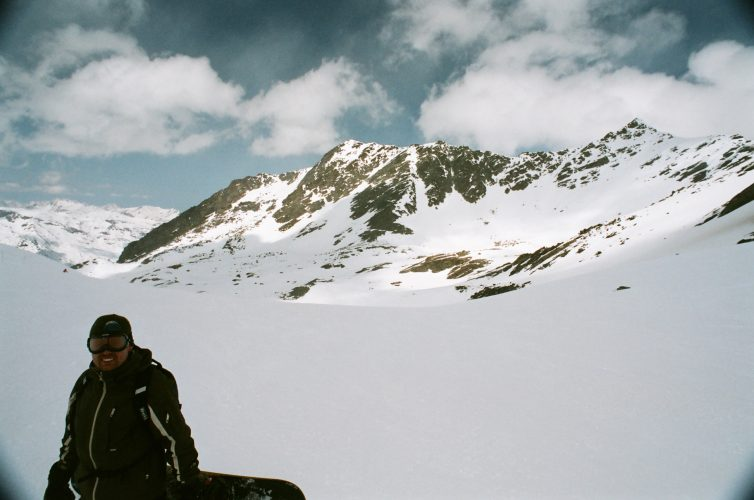
\includegraphics[width=\textwidth]{TagTree/Flickrimg/7a6b7ae7-7afb-3f90-92df-e67c0bd22a8a.jpeg}
                \caption{\textbf{Seen}: film, france \\ \textbf{Unseen}: holiday, \\ sky, snow \\ \textbf{Predicted}: paris, europe, bw }
                \label{fig:negex1}
        \end{subfigure}%
	\; \vline
        \; %add desired spacing between images, e. g. ~, \quad, \qquad etc.
          %(or a blank line to force the subfigure onto a new line)
        \begin{subfigure}[b]{0.17\textwidth}
                
\includegraphics[width=0.8\textwidth]{TagTree/Flickrimg/ec4436dd-57b3-36af-94f6-64cf05294886.jpeg}
                \caption{\textbf{Seen}: china, family \\ \textbf{Unseen}: live, summer, \\ usa  \\ \textbf{Predicted}: photography, christmas, photo }
                \label{fig:negex2}
        \end{subfigure}%
	\; \vline
        \; %add desired spacing between images, e. g. ~, \quad, \qquad etc.
          %(or a blank line to force the subfigure onto a new line)
        \begin{subfigure}[b]{0.16\textwidth}
                
\includegraphics[width=0.8\textwidth]{TagTree/Flickrimg/bf51a02f-baa1-3861-a300-12b5f654c456.jpeg}
                \caption{\textbf{Seen}: canada, \\ ocean \\ \textbf{Unseen}: red, sky, sunset \\ \textbf{Predicted}: sea, beach, water }
                \label{fig:negex3}
        \end{subfigure}%
	\; \vline
        \; %add desired spacing between images, e. g. ~, \quad, \qquad etc.
          %(or a blank line to force the subfigure onto a new line)
        \begin{subfigure}[b]{0.17\textwidth}
                
\includegraphics[width=0.8\textwidth]{TagTree/Flickrimg/b339e52a-b87e-347a-8ba8-12502fc11443.jpeg}
                \caption{\textbf{Seen}: autumn, \\ black\\ \textbf{Unseen}: light, macro, night \\ \textbf{Predicted}: white, nature, bw }
                \label{fig:negex4}
        \end{subfigure}%
	\; \vline
        \; %add desired spacing between images, e. g. ~, \quad, \qquad etc.
          %(or a blank line to force the subfigure onto a new line)
        \begin{subfigure}[b]{0.18\textwidth}
                
\includegraphics[width=0.45\textwidth]{TagTree/Flickrimg/acf2533e-69ac-3e2e-8eab-e024ca9682fd.jpeg}
                \caption{\textbf{Seen}: car, green \\ \textbf{Unseen}: photo, washington, white \\ \textbf{Predicted}: red, spring, nature }
                \label{fig:negex5}
        \end{subfigure}
        \caption[Example images where LS-SA method gave 0\% tag prediction accuracy when the first two tags were seen and the next three were unseen and predicted. ]{Example images where LS-SA method gave 0\% tag prediction accuracy when the first two tags were seen and the next three were unseen and predicted. Also provided are the tags that were predicted by the LS-SA method. The Flickr owner and photo ids of these images
are (king-edward@4061393892) , (familymwr@4928996212) , (alejandroerickson@7730525250) , (wwarby@5145467790) ,  (1968-dodge-charger@5507716438)  respectively. \textbf{Seen: ($\mathcal{T}_{i,Seen}$); Unseen: ($\mathcal{T}_i \setminus  \mathcal{T}_{i,Seen}$); Predicted: ($\mathbb{P}_i$)} as per Section~\ref{subsec:TagPred}. }  \label{fig:negativeExs}
\end{figure*}



\section{Discussion}
\label{sec:Discussion}
\begin{figure*}[t!]
\centering
\minipage{0.49\textwidth}
\centering
  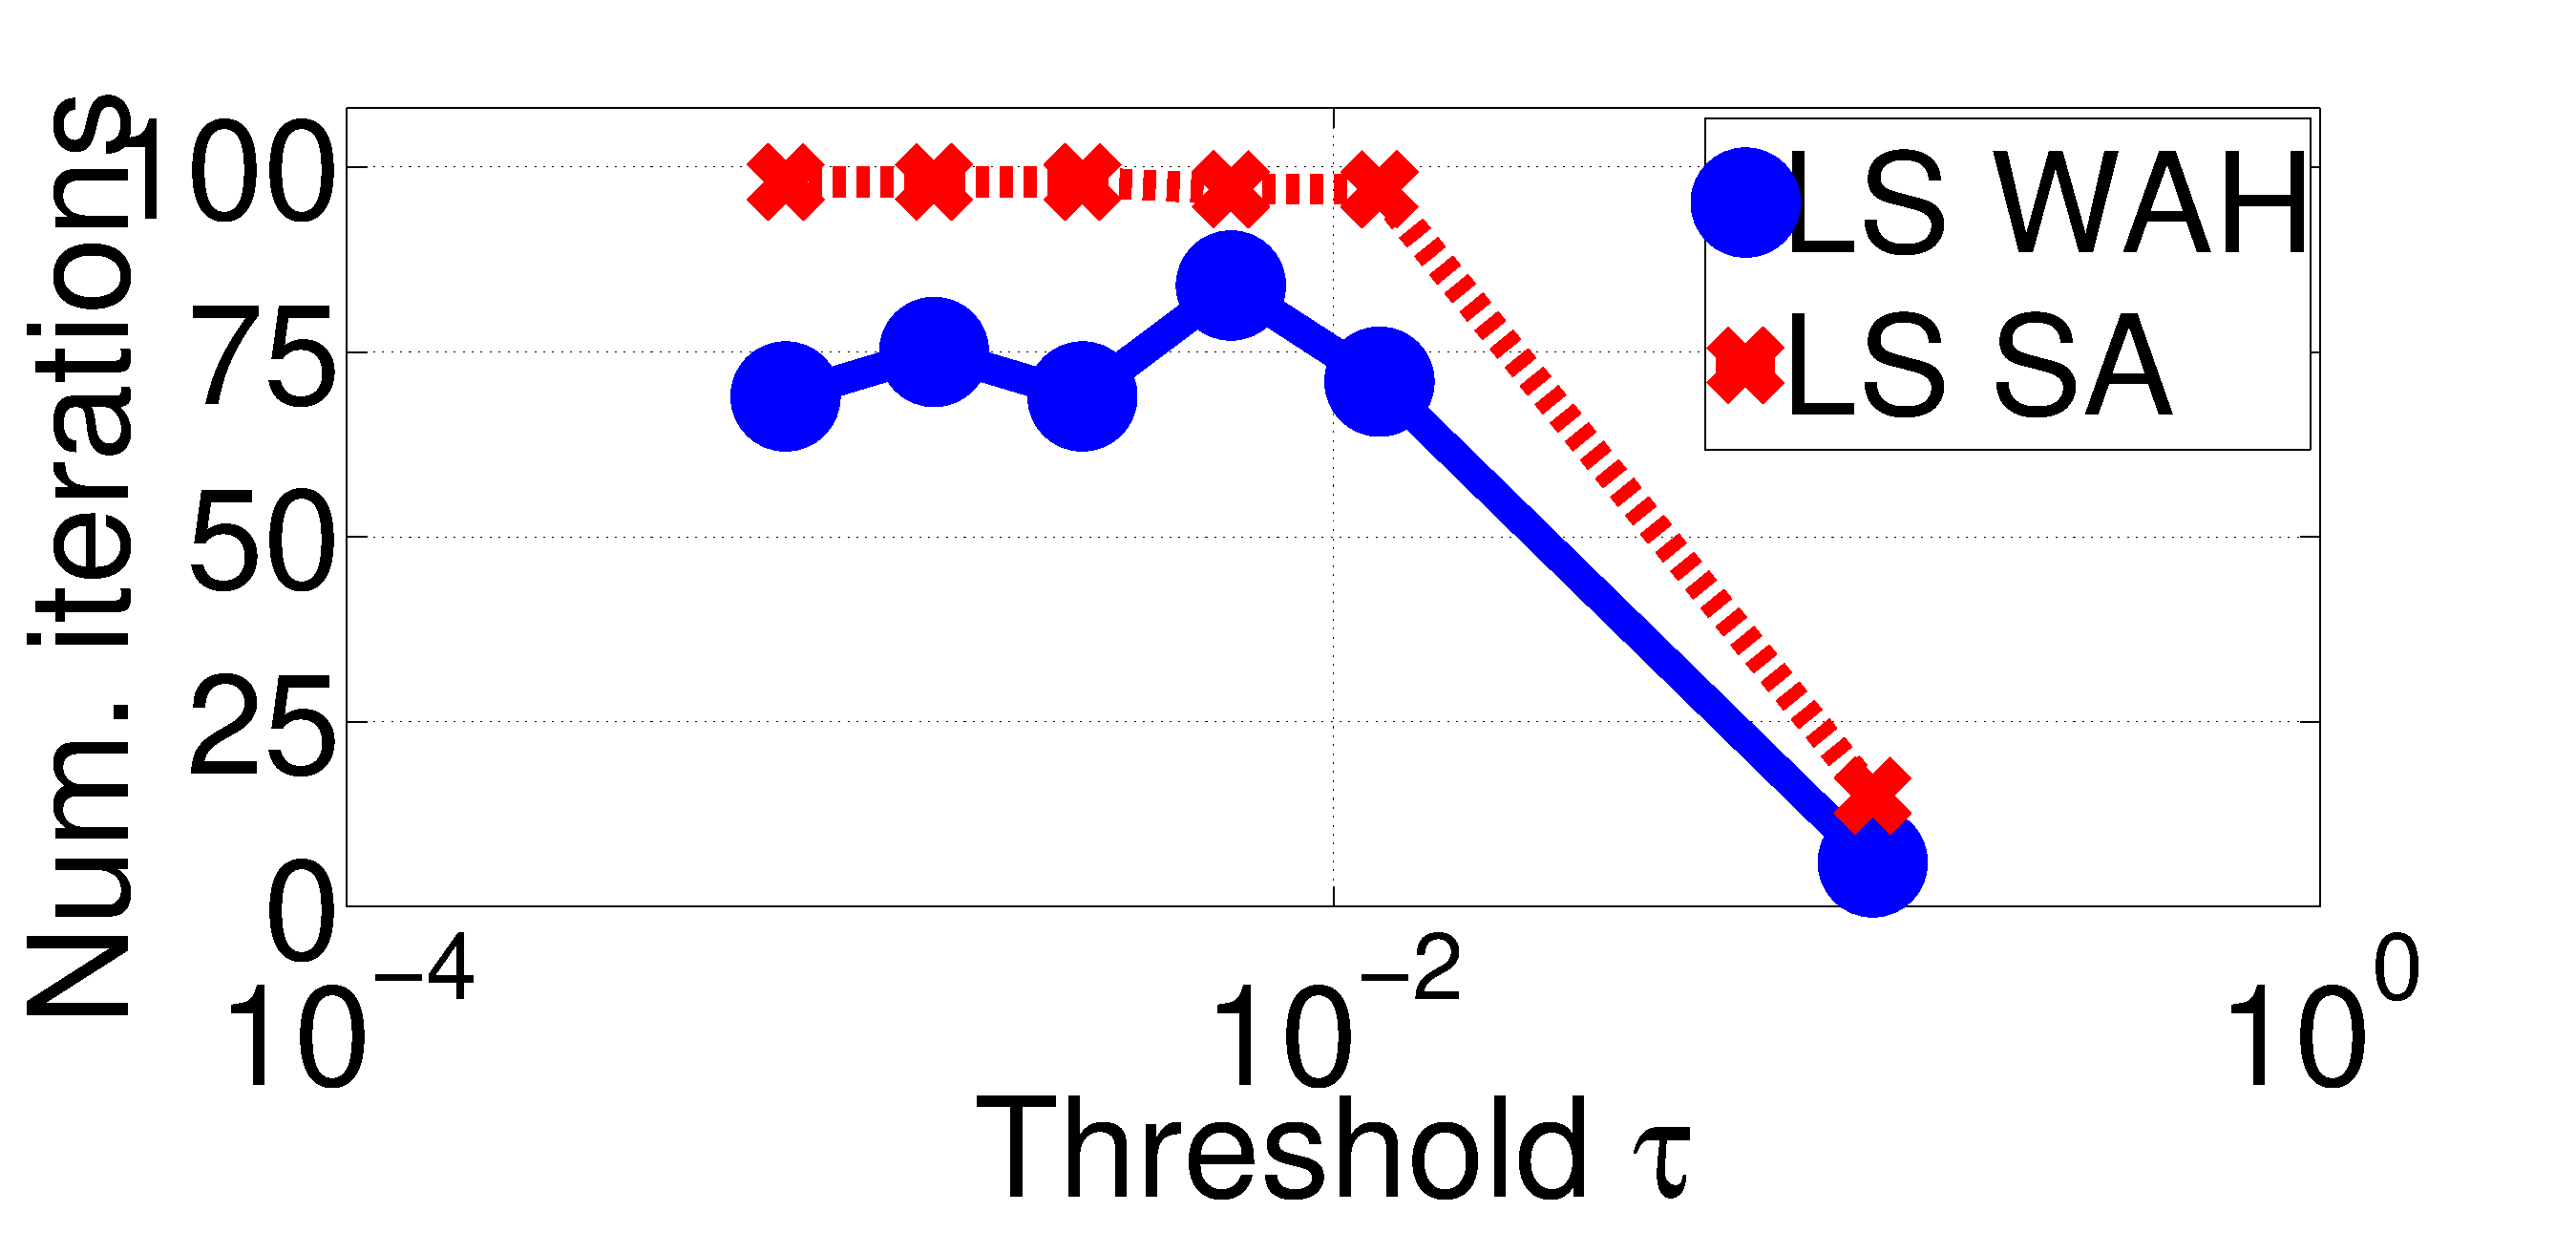
\includegraphics[width=\linewidth]{TagTree/RebuttalNIterationsWithTauNew} 
%  \includegraphics[width=\linewidth]{TagTree/RebuttalNCandidatesWithTau}
  \caption{Variation of number of iterations with $\tau$}
  \label{fig:TauNIterations}
%\end{centering}
\endminipage %\hfill
\minipage{0.49\textwidth}
  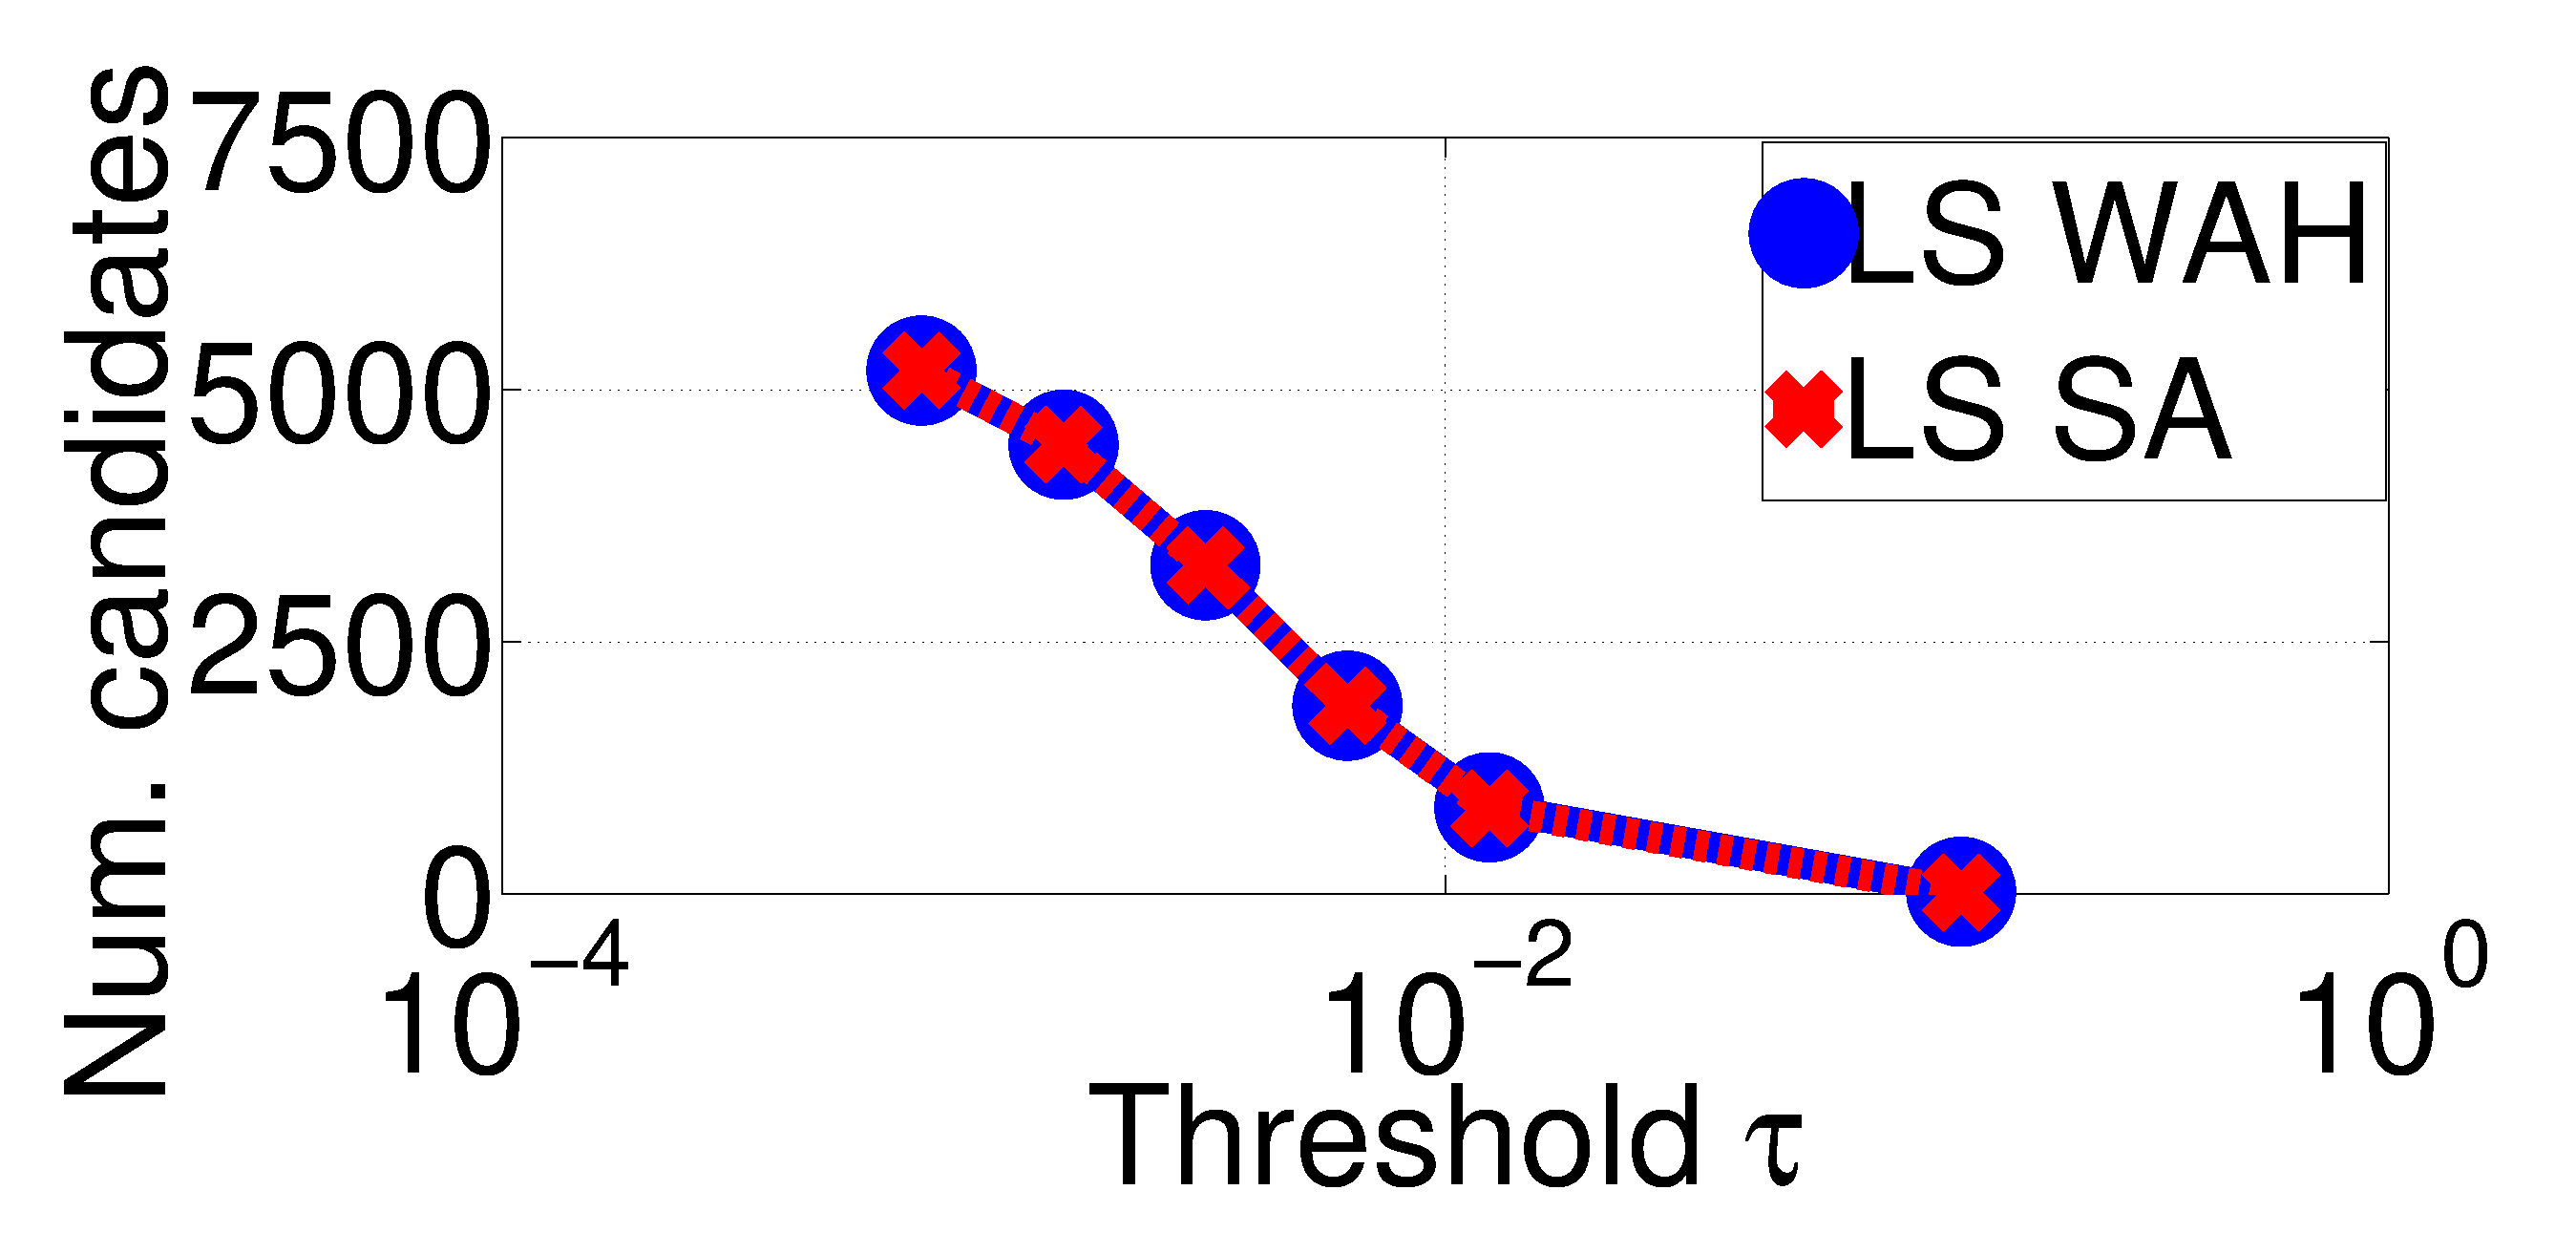
\includegraphics[width=\linewidth]{TagTree/RebuttalNCandidatesWithTauNew}
  \caption{Variation of number of candidate neighbors with $\tau$}
  \label{fig:TauNCandidate}
\endminipage %\hfill
\end{figure*} 
\begin{figure*}[t!]
\minipage{0.49\textwidth}
%  \includegraphics[width=\linewidth]{TagTree/RebuttalNCandidatesWithTau}
  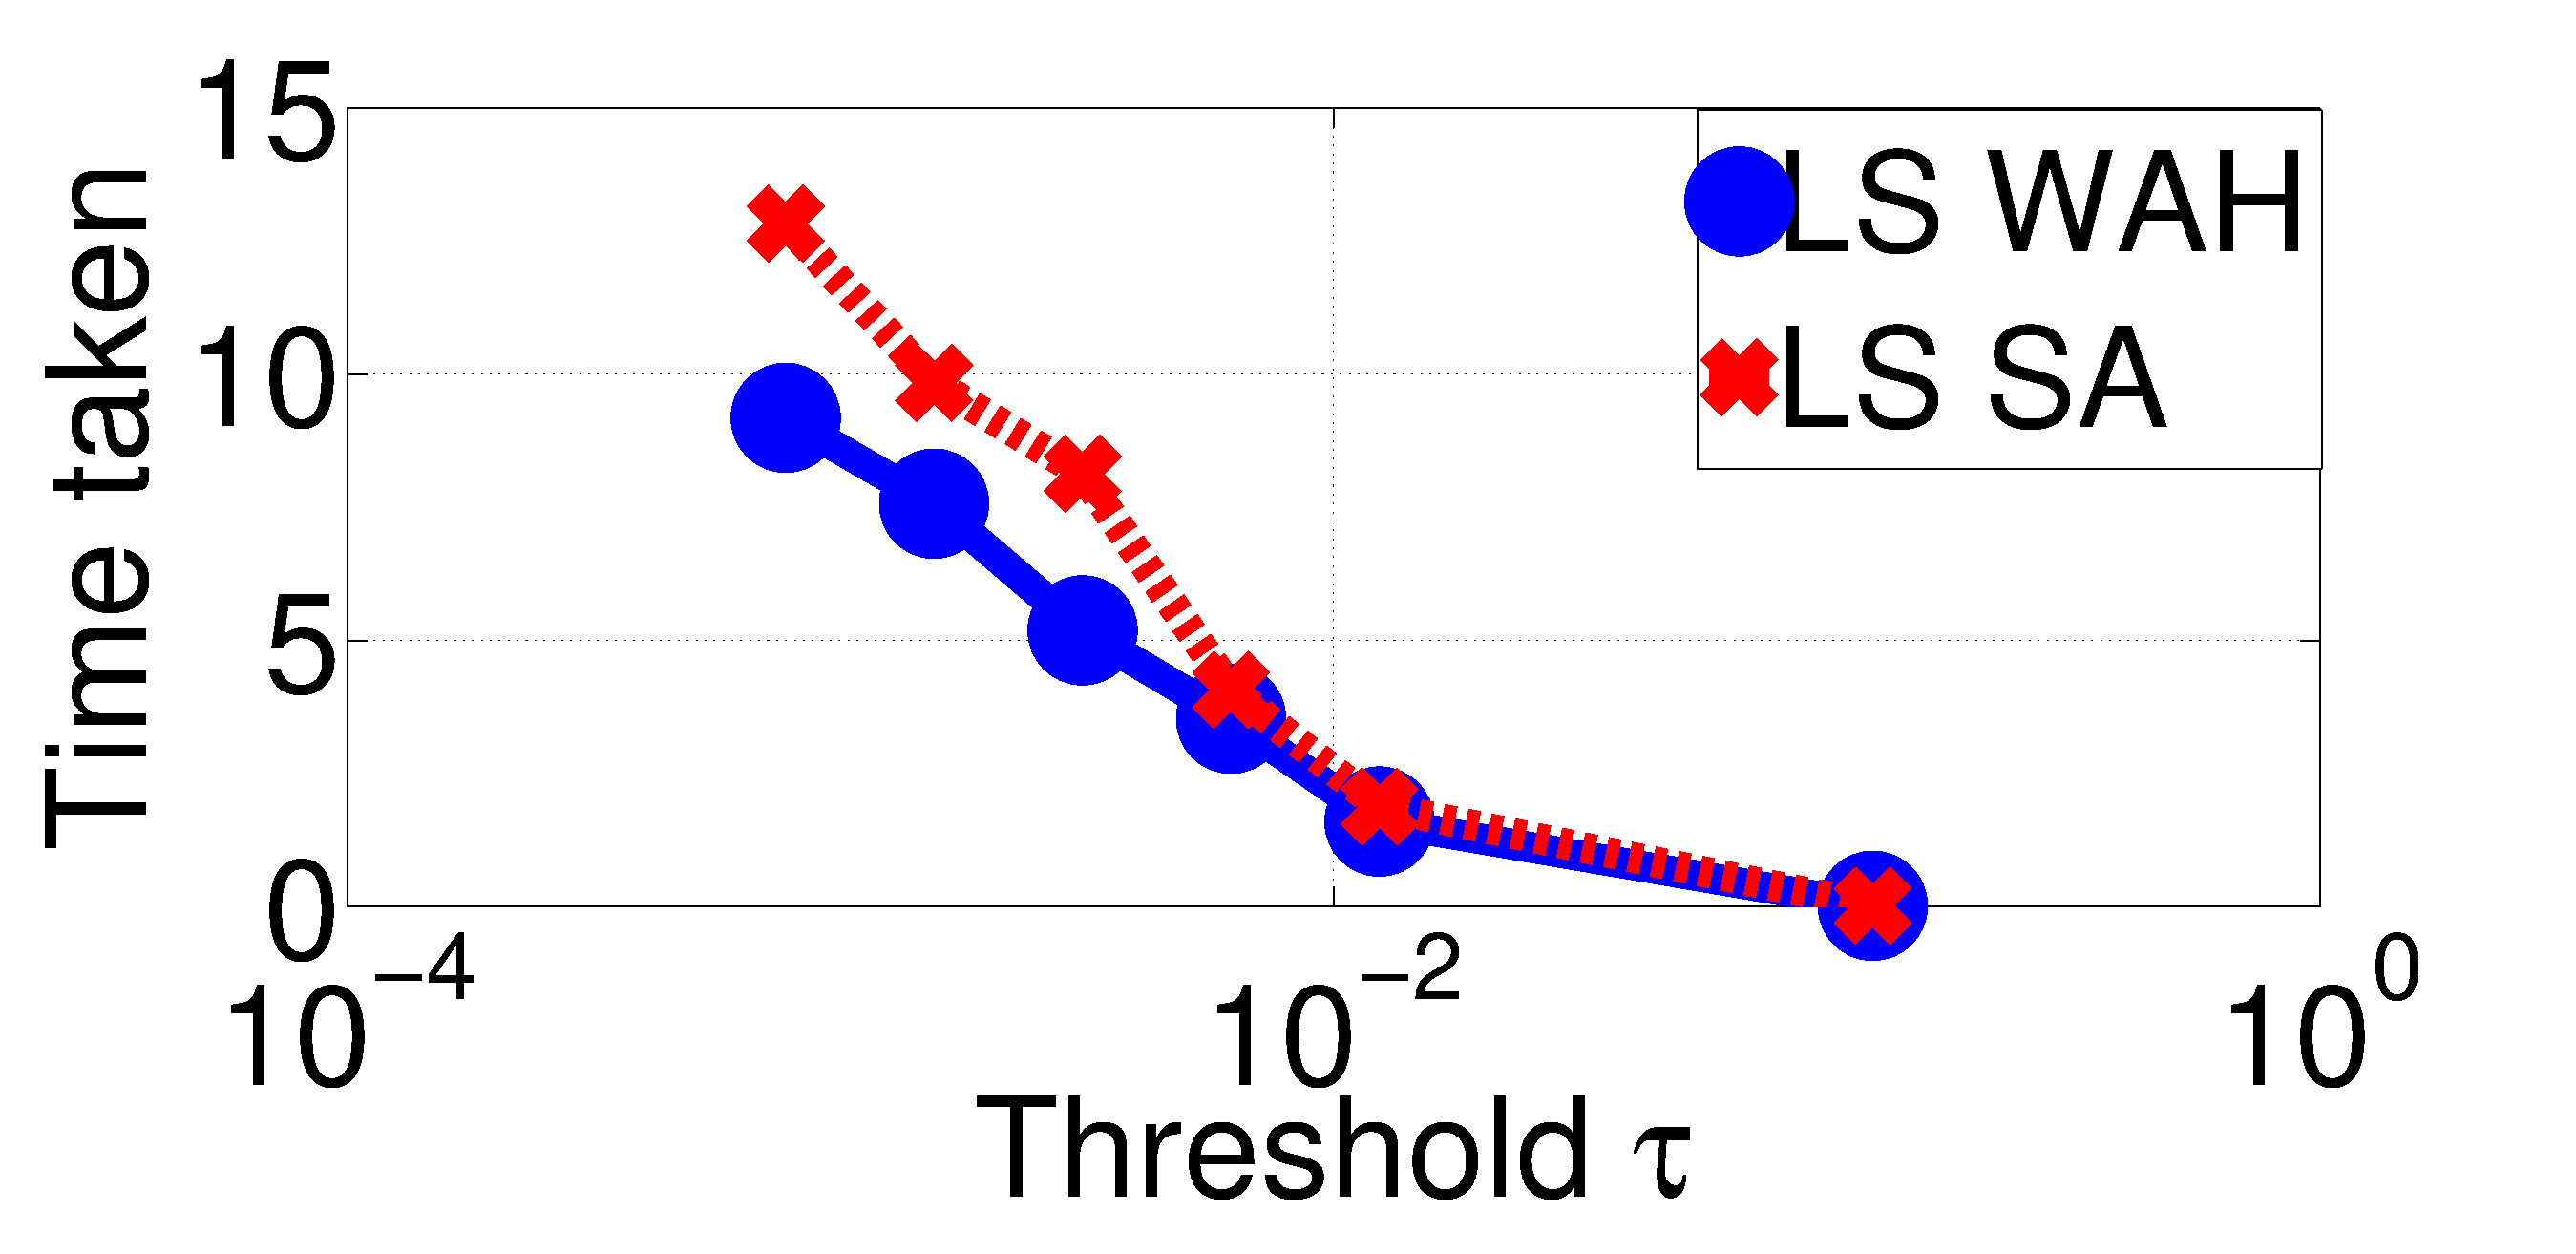
\includegraphics[width=\linewidth]{TagTree/TimeNIterationsWithTau}
  \caption{Variation of time (hours) taken by local search to converge}
  \label{fig:TauTimetaken}
\endminipage %\hfill
%\vspace{0.1in}
\minipage{0.49\textwidth}%
  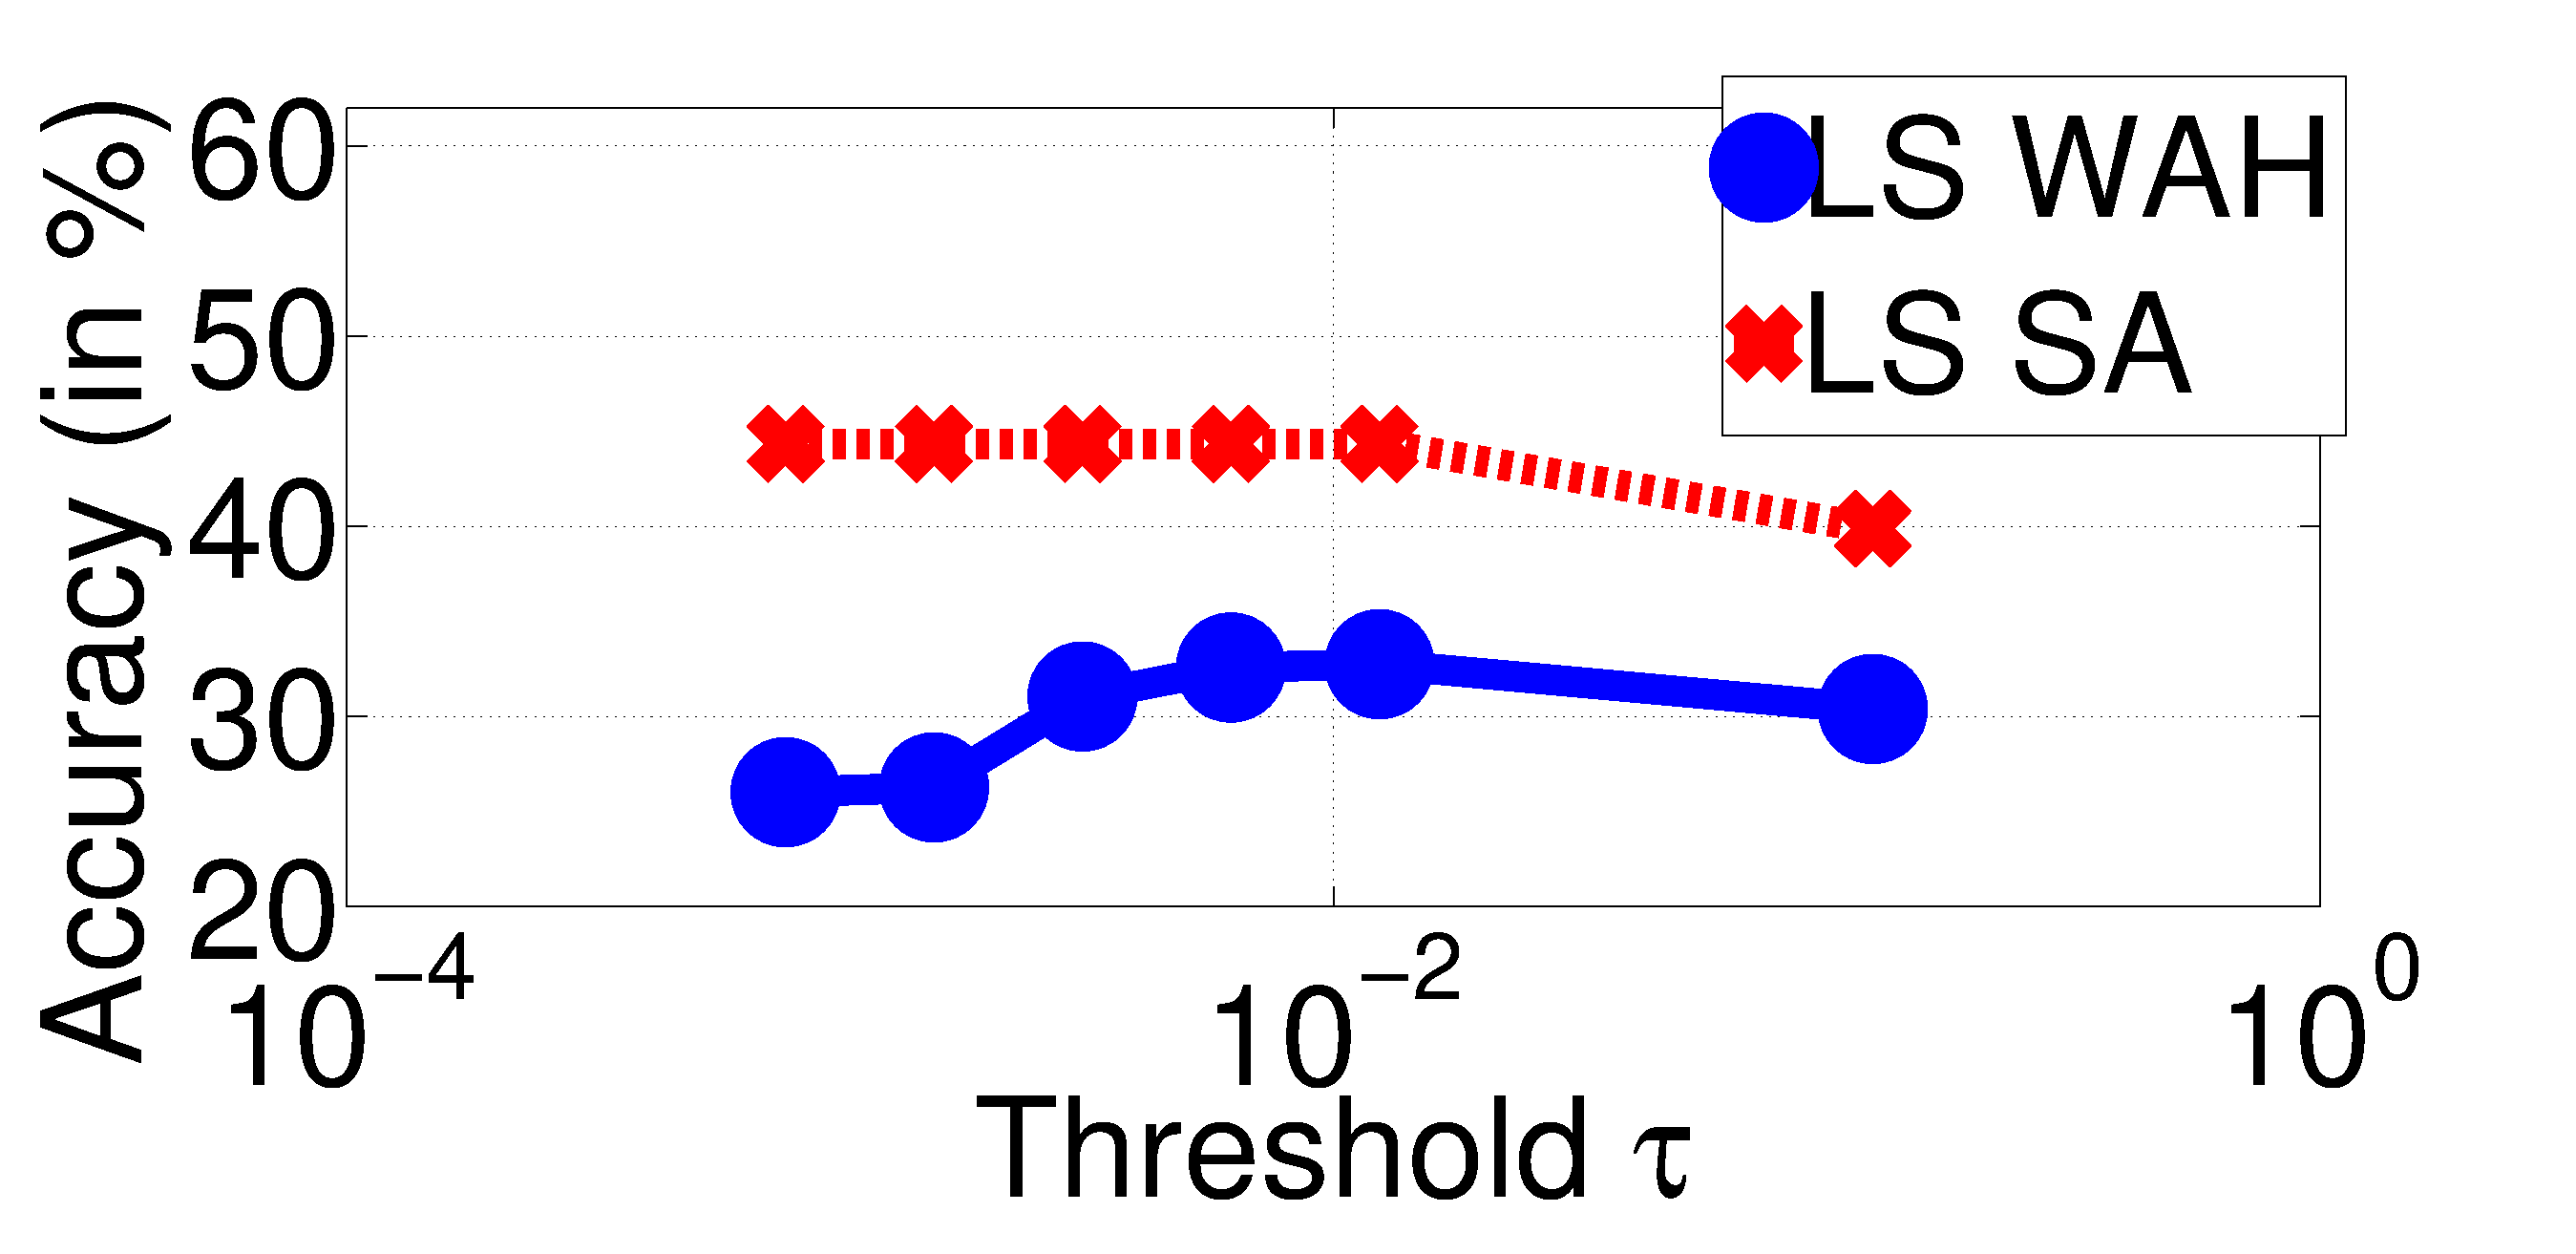
\includegraphics[width=\linewidth]{TagTree/RebuttalAccuracyWithTauNew}
%  \includegraphics[width=\linewidth]{RebuttalNCandidatesWithTau}
  \caption{Variation of the Average Tag Prediction Accuracy with $\tau$}
  \label{fig:TauAccuracy}
\endminipage
\end{figure*}

In this section, we provide a discussion on the key insights and observations made during the course of study on ontological tag trees. \\
\indent As outlined in Section~\ref{sec:ConstructionTree}, the motivation for the objective function (\ref{eq:ObjFnWeightedHops})  in the proposed approach is that in order to get a lower value for (\ref{eq:ObjFnWeightedHops}), it is more important to separate the tags $t_i$ and $t_j$ having high $J_{\mathcal{T}}(i,j)$ with less number of hops, as compared to the tags with low $J_{\mathcal{T}}(i,j)$. However, separating the latter set of tags by fewer hops would also lower the value of  (\ref{eq:ObjFnWeightedHops}). Since (\ref{eq:ObjFnWeightedHops}) attempts to minimize the weighted number of hops between tag pairs, a local search in the space of all possible trees on $\mathcal{T}$ would lead to connecting most tags to a central tag, thus forming a star graph. Such a minimum weighted hops spanning tree problem on an all connected graph can be solved in polynomial time using Gomory-Hu trees~\cite{panigrahi2008gomory}, however star graphs need not reflect the true relationship between tags in a corpus. In order to ensure that the proposed approach does not induce artificial structures because of bias of the objective function, we constrain the search space to be spanning trees of a suitably constructed Similarity Graph with the help of a threshold $\tau$, as outlined in Section~\ref{sec:refinement}. Experimentally, constraining as above does succeed in ensuring that we do not get a star graph. However upon visual inspection, the proposed approach yields star subtrees connected through their centers.
The objective function (\ref{eq:ObjFnSimApprox}) in comparison has no such bias for shorter trees and as a result, the results for proposed approach using (\ref{eq:ObjFnSimApprox}) outperform those using (\ref{eq:ObjFnWeightedHops}). 
\hl{Figures {\ref{fig:TauNIterations}} through {\ref{fig:TauAccuracy}} show the variation of different aspects of constructed tag trees with $\tau$ for 117 Flickr tags. Fig.~{\ref{fig:TauNCandidate}} shows that with increasing $\tau$, the number of tag trees that are eligible candidates in an iteration of the local search, drops drastically for both LS-WAH and LS-SA. As discussed above, a lenient $\tau$ leads to the LS-WAH based local search converging to star graphs which are an artefact of the procedure and not of the true relationships between the tags. As a result, for lower $\tau$, the performance of LS-WAH based approach degrades substantially as can be seen in Fig.~{\ref{fig:TauAccuracy}}. For large values of $\tau$, the number of candidate neighbors at each iteration of the local search become less. This constrains the local search and prevents it from attaining a lower value for the objective function ({\ref{eq:ObjFnSimApprox}}). This leads to a drop in the performance of LS-SA as can be seen in Fig.~{\ref{fig:TauAccuracy}}. We have chosen a threshold as the median of the pair-wise jaccard similarity values since it offers a convenient trade-off between number of candidates and performance for LS-SA. } 

At each iteration of the proposed approach, there are $O(N^2)$ neighbors of a tree to explore, where $N=\mid \mathcal{T} \mid$. Calculating the pair-wise distances (or hops) and computing (\ref{eq:ObjFnWeightedHops}) or (\ref{eq:ObjFnSimApprox}) requires $O(N^2)$ operations per neighbor~\cite{ford2010flows}. Thus, the complexity of the proposed approach, for either objective function, is $O(N^4)$ per iteration. \hl{A bottleneck of the proposed tag tree construction approach is the time taken for local search to terminate. Fig.~{\ref{fig:TauTimetaken}} shows the variation of the time taken by the proposed local search based approach, with respect to $\tau$. Matlab on a 2.9GHz, 8GB RAM 4 core processor is used.} One way to reduce the time taken at each iteration is to reduce the number of neighbors. This is achieved by constraining the solution space to spanning trees of a Similarity Graph. While the order of complexity at each iteration remains at $O(N^4)$, the time taken is much less. For instance, when $\tau$ is chosen as median of the pair-wise jaccard similarity values as in Section~\ref{sec:Expts}, the time taken is nearly half of the time taken when $\tau=0$, which corresponds to having search space as all possible trees on $\mathcal{T}$. 
%Thus, confining the local search to spanning trees of the Similarity Graph helps ensure that the proposed approach using objective function (\ref{eq:ObjFnWeightedHops}) gives a non-trivial solution. Since the proposed approach using objective function (\ref{eq:ObjFnSimApprox}) has no such bias 
%It is not necessary for the correctness of the proposed approach using (\ref{eq:ObjFnSimApprox}) to use the Similarity Graph.
%Thus, the Similarity Graph has different uses for objective functions (\ref{eq:ObjFnWeightedHops}) and (\ref{eq:ObjFnSimApprox}). While in the case of the former, it helps to ensure that the proposed approach leads to a non-trivial solution, in the latter case, its only use is to speed up the search for a local optimum. 
Thus, for the proposed approach using objective function (\ref{eq:ObjFnWeightedHops}), constraining the local search to spanning trees of a Similarity Graph is necessary to ensure that we do not get a trivial solution.  Doing so also makes the local search faster. \hl{As compared to this, for the proposed approach using objective function ({\ref{eq:ObjFnSimApprox}}), using a Similarity Graph only makes the optimum search faster as can be seen in the reduced number of candidates in Fig.~{\ref{fig:TauNCandidate}} and the reduced number of iterations to converge, as shown in Fig.~{\ref{fig:TauNIterations}}}. 



\hl{Intuitively, using ({\ref{eq:ObjFnSimApprox}}) as the objective function minimizes the weighted L1 norm of the difference between pair-wise jaccard similarity and the similarity estimated using a tag tree, thus trying to approximate the normalized symmetric second order statistics of a corpus using a tree on the set of tags}. We have chosen weighted L1 norm since it was observed to lead to the best results across different corpora among other variants such as L1, L2 and weighted L2 norm. Implementation of the similarity estimated using a tag tree (\ref{eq:ProdSimSimilarityCalculate}) can be conveniently done by using Logarithms and Ford Fulkerson Algorithm~\cite{ford2010flows}. Also, since the LS-SA approximates the pair-wise similarities $J_{\mathcal{T}}(i,j)$ in $O(N)$ as compared to $O(N^2)$, approaches such as {\cite{sigurbjornsson2008flickr}} that utilize $J_{\mathcal{T}}(i,j)$ lead to equal or only marginally better performance, despite having several orders higher space requirement. \\


\section{Conclusions and Future Work}

In this section we summarize the research contributions of this chapter, key practical insights, and advantages and limitations as compared to existing expert systems. We also discuss limitations of our work, and provide several suggestions for future research directions. 

We have proposed ontological tag trees to enable expert systems address the sparsity of folksonomies effectively and in a space efficient manner. Ontological tag trees or tag trees are defined as simple trees on the set of tags in a corpus. The construction of tag trees is formulated as an optimization problem on corpus based statistics, and is solved through a novel local search based approach. We have shown that this approach can be used to build tag trees for tags obtained from two corpora, one composed of noisily annotated Flickr images and the other composed of cleanly annotated stock images. To validate the utility of the constructed ontological tag tree, we proposed two evaluation tasks involving tag prediction in images.  We have demonstrated that for the task of predicting the unseen tags of a given image with a partially observed set of tags, the proposed ontological tag trees outperform those constructed using only semantic relationships, or tag graphs constructed using commonly used techniques that have comparable space requirements. In the second task, we have shown that the tag tree obtained from the proposed approach makes the process of using appropriate classifiers to tag an untagged test image more efficient. Robustness analysis shows that the proposed approach is fairly robust to tag noise and differences between the training and test set distributions.

Compared to previous expert systems, our work offers significant advantages. In addition, several key insights can be derived from our study. Since expert systems such as~\cite{MohdSemantic13} based on only semantic relationships fail to capture the data-specific relationships between tags, their performance is significantly lower on data-driven tasks than that of ontological tag trees constructed using the proposed approach. This is demonstrated through evaluations in Section~\ref{sec:Expts}. In addition, we show that even though ontological tag trees have space requirement of only $O(N)$ for $N$ tags, as compared to $O(N^2)$ for tag graphs, tag trees can provide equal or better performance than several existing expert systems on the evaluation tasks. Particularly, compared to~\cite{sigurbjornsson2008flickr} which may require 27 terabytes of space to store pair-wise similarities, our approach requires less than 50 megabytes, and still achieves almost equal performance. Ontological tag trees can thus offer a very convenient method for expert systems to capture corpus based relationships for tasks such as tag prediction, and efficient resource classification. The significant savings in space requirement facilitates practical deployment of the expert systems even on computing devices that do not have gigantic memory available. The third key advantage of using ontological tag trees is that their construction does not depend on the availability of content-based features (such as textual or visual features). Thus as compared to previous expert systems such as~\cite{li2009learning}, \cite{wu2009distance}, \cite{HsiehCollab09}, \cite{ChenEstim15}, \cite{SunLang11}, our approach can help alleviate sparsity of online folksonomies even in domains where extracting content-based features may be inefficient or infeasible~\cite{huang2010text}, \cite{song2010taxonomic}, \cite{zanetti2008walk}, \cite{yin2009exploring}. Lastly, as discussed in Section~\ref{sec:Discussion}, the performance of the LS-SA approach is significantly better than that of the LS-WAH approach. It can thus be recommended that the LS-SA approach be used to construct ontological tag trees. 


While the proposed ontological tag trees can help expert systems achieve high performance in a space efficient manner, there are certain limitations of the proposed approach. As discussed in Section~\ref{sec:Discussion}, the time taken per iteration of the local search based tag tree construction approach varies as $O(N^4)$. For large number of tags, the total time taken to construct tag trees can be high. In addition, the tag trees only capture undirected weighted relationships between tags. As a result, any directed relationships that may be present in the corpus (for example subsumption relationships~\cite{SubsumptionFlickr}) are lost by the constructed tag trees. 


We provide several suggestions for future work directions based on our work. 
Since the tag tree construction approach has a limitation of high time requirement, one direction of future work could be to make the proposed approach faster by choosing a higher or an adaptive $\tau$, with the possible trade-off being increasing the constraint on the local search, thereby achieving a sub-optimal tag tree. Another direction of future work could be to keep a low $\tau$ but develop distributed and possibly approximated versions of the proposed approach, such that available distributed clusters, for example Amazon EC2 cloud server~\cite{AmazonEC2}, can be leveraged. 
In the current work, the LS-SA approach can be thought of as approximating the symmetric second order corpus statistics. An extension of the work could be to construct tag structures that approximate higher order corpus statistics. 
In addition, future work could utilize the constructed tag trees for other practical applications such as tag recommendation: given set of tags associated with a test images, which $additional$ tags would you associate with the image? Removal of potentially noisy tags can also be studied based on whether a tag appears too far in the tree from other tags associated with a given image. Lastly, a hierarchical taxonomy could be constructed in future, where the edges between the nodes are directed, by adopting similar techniques and using the co-occurrence data from the corpus. 

\section{Acknowledgments} 
We thank the anonymous WWW 2014 and Elsevier Expert Systems with Applications reviewers for their feedback and comments on the work. This research was partially supported by an internship at Yahoo Labs, and partially by the Center for Wireless Communications at University of California San Diego. 

Chapter 3, in part, contains material as it appears in the Proceedings of the companion publication of the 23rd International Conference on World Wide Web (WWW '14). ``Construction of Tag Ontological Graphs by Locally Minimizing Weighted Average Hops''. Chetan Verma, Vijay Mahadevan, Nikhil Rasiwasia, Gaurav Aggarwal, Ravi Kant, Alejandro Jaimes, Sujit Dey. The dissertation author was the primary investigator and author of this paper. 

Chapter 3, in part, contains material as it appears in Elsevier Expert Systems with Applications. ``Construction and Evaluation of Ontological Tag Trees''. Chetan Verma, Vijay Mahadevan, Nikhil Rasiwasia, Gaurav Aggarwal, Ravi Kant, Alejandro Jaimes, Sujit Dey. The dissertation author was the primary investigator and author of this paper. 






